% Options for packages loaded elsewhere
\PassOptionsToPackage{unicode}{hyperref}
\PassOptionsToPackage{hyphens}{url}
%
\documentclass[
]{book}
\usepackage{amsmath,amssymb}
\usepackage{iftex}
\ifPDFTeX
  \usepackage[T1]{fontenc}
  \usepackage[utf8]{inputenc}
  \usepackage{textcomp} % provide euro and other symbols
\else % if luatex or xetex
  \usepackage{unicode-math} % this also loads fontspec
  \defaultfontfeatures{Scale=MatchLowercase}
  \defaultfontfeatures[\rmfamily]{Ligatures=TeX,Scale=1}
\fi
\usepackage{lmodern}
\ifPDFTeX\else
  % xetex/luatex font selection
\fi
% Use upquote if available, for straight quotes in verbatim environments
\IfFileExists{upquote.sty}{\usepackage{upquote}}{}
\IfFileExists{microtype.sty}{% use microtype if available
  \usepackage[]{microtype}
  \UseMicrotypeSet[protrusion]{basicmath} % disable protrusion for tt fonts
}{}
\makeatletter
\@ifundefined{KOMAClassName}{% if non-KOMA class
  \IfFileExists{parskip.sty}{%
    \usepackage{parskip}
  }{% else
    \setlength{\parindent}{0pt}
    \setlength{\parskip}{6pt plus 2pt minus 1pt}}
}{% if KOMA class
  \KOMAoptions{parskip=half}}
\makeatother
\usepackage{xcolor}
\usepackage{color}
\usepackage{fancyvrb}
\newcommand{\VerbBar}{|}
\newcommand{\VERB}{\Verb[commandchars=\\\{\}]}
\DefineVerbatimEnvironment{Highlighting}{Verbatim}{commandchars=\\\{\}}
% Add ',fontsize=\small' for more characters per line
\usepackage{framed}
\definecolor{shadecolor}{RGB}{248,248,248}
\newenvironment{Shaded}{\begin{snugshade}}{\end{snugshade}}
\newcommand{\AlertTok}[1]{\textcolor[rgb]{0.94,0.16,0.16}{#1}}
\newcommand{\AnnotationTok}[1]{\textcolor[rgb]{0.56,0.35,0.01}{\textbf{\textit{#1}}}}
\newcommand{\AttributeTok}[1]{\textcolor[rgb]{0.13,0.29,0.53}{#1}}
\newcommand{\BaseNTok}[1]{\textcolor[rgb]{0.00,0.00,0.81}{#1}}
\newcommand{\BuiltInTok}[1]{#1}
\newcommand{\CharTok}[1]{\textcolor[rgb]{0.31,0.60,0.02}{#1}}
\newcommand{\CommentTok}[1]{\textcolor[rgb]{0.56,0.35,0.01}{\textit{#1}}}
\newcommand{\CommentVarTok}[1]{\textcolor[rgb]{0.56,0.35,0.01}{\textbf{\textit{#1}}}}
\newcommand{\ConstantTok}[1]{\textcolor[rgb]{0.56,0.35,0.01}{#1}}
\newcommand{\ControlFlowTok}[1]{\textcolor[rgb]{0.13,0.29,0.53}{\textbf{#1}}}
\newcommand{\DataTypeTok}[1]{\textcolor[rgb]{0.13,0.29,0.53}{#1}}
\newcommand{\DecValTok}[1]{\textcolor[rgb]{0.00,0.00,0.81}{#1}}
\newcommand{\DocumentationTok}[1]{\textcolor[rgb]{0.56,0.35,0.01}{\textbf{\textit{#1}}}}
\newcommand{\ErrorTok}[1]{\textcolor[rgb]{0.64,0.00,0.00}{\textbf{#1}}}
\newcommand{\ExtensionTok}[1]{#1}
\newcommand{\FloatTok}[1]{\textcolor[rgb]{0.00,0.00,0.81}{#1}}
\newcommand{\FunctionTok}[1]{\textcolor[rgb]{0.13,0.29,0.53}{\textbf{#1}}}
\newcommand{\ImportTok}[1]{#1}
\newcommand{\InformationTok}[1]{\textcolor[rgb]{0.56,0.35,0.01}{\textbf{\textit{#1}}}}
\newcommand{\KeywordTok}[1]{\textcolor[rgb]{0.13,0.29,0.53}{\textbf{#1}}}
\newcommand{\NormalTok}[1]{#1}
\newcommand{\OperatorTok}[1]{\textcolor[rgb]{0.81,0.36,0.00}{\textbf{#1}}}
\newcommand{\OtherTok}[1]{\textcolor[rgb]{0.56,0.35,0.01}{#1}}
\newcommand{\PreprocessorTok}[1]{\textcolor[rgb]{0.56,0.35,0.01}{\textit{#1}}}
\newcommand{\RegionMarkerTok}[1]{#1}
\newcommand{\SpecialCharTok}[1]{\textcolor[rgb]{0.81,0.36,0.00}{\textbf{#1}}}
\newcommand{\SpecialStringTok}[1]{\textcolor[rgb]{0.31,0.60,0.02}{#1}}
\newcommand{\StringTok}[1]{\textcolor[rgb]{0.31,0.60,0.02}{#1}}
\newcommand{\VariableTok}[1]{\textcolor[rgb]{0.00,0.00,0.00}{#1}}
\newcommand{\VerbatimStringTok}[1]{\textcolor[rgb]{0.31,0.60,0.02}{#1}}
\newcommand{\WarningTok}[1]{\textcolor[rgb]{0.56,0.35,0.01}{\textbf{\textit{#1}}}}
\usepackage{longtable,booktabs,array}
\usepackage{calc} % for calculating minipage widths
% Correct order of tables after \paragraph or \subparagraph
\usepackage{etoolbox}
\makeatletter
\patchcmd\longtable{\par}{\if@noskipsec\mbox{}\fi\par}{}{}
\makeatother
% Allow footnotes in longtable head/foot
\IfFileExists{footnotehyper.sty}{\usepackage{footnotehyper}}{\usepackage{footnote}}
\makesavenoteenv{longtable}
\usepackage{graphicx}
\makeatletter
\def\maxwidth{\ifdim\Gin@nat@width>\linewidth\linewidth\else\Gin@nat@width\fi}
\def\maxheight{\ifdim\Gin@nat@height>\textheight\textheight\else\Gin@nat@height\fi}
\makeatother
% Scale images if necessary, so that they will not overflow the page
% margins by default, and it is still possible to overwrite the defaults
% using explicit options in \includegraphics[width, height, ...]{}
\setkeys{Gin}{width=\maxwidth,height=\maxheight,keepaspectratio}
% Set default figure placement to htbp
\makeatletter
\def\fps@figure{htbp}
\makeatother
\setlength{\emergencystretch}{3em} % prevent overfull lines
\providecommand{\tightlist}{%
  \setlength{\itemsep}{0pt}\setlength{\parskip}{0pt}}
\setcounter{secnumdepth}{5}
\usepackage{booktabs}
\ifLuaTeX
  \usepackage{selnolig}  % disable illegal ligatures
\fi
\usepackage[]{natbib}
\bibliographystyle{apalike}
\IfFileExists{bookmark.sty}{\usepackage{bookmark}}{\usepackage{hyperref}}
\IfFileExists{xurl.sty}{\usepackage{xurl}}{} % add URL line breaks if available
\urlstyle{same}
\hypersetup{
  pdftitle={Lerne Python, indem du Spiele entwickels},
  pdfauthor={Alexander (Sasha) Pastukhov},
  hidelinks,
  pdfcreator={LaTeX via pandoc}}

\title{Lerne Python, indem du Spiele entwickels}
\author{Alexander (Sasha) Pastukhov}
\date{2023-10-23}

\begin{document}
\maketitle

{
\setcounter{tocdepth}{1}
\tableofcontents
}
\hypertarget{intro}{%
\chapter{Einleitung}\label{intro}}

Dieses Buch wird dich das Programmieren lehren. Hoffentlich auf eine spaßige Art und Weise, denn wenn es etwas Befriedigenderes gibt als ein Videospiel zu spielen, dann ist es, eines zu erstellen. Obwohl es für den Kurs \emph{``Python für soziale und experimentelle Psychologie''} geschrieben wurde, ist mein Hauptziel nicht, dir Python an sich beizubringen. Python ist ein fantastisches Werkzeug (mehr dazu später), aber es ist nur eine von vielen existierenden Programmiersprachen. Mein ultimatives Ziel ist es, dir dabei zu helfen, allgemeine Programmierfähigkeiten zu entwickeln, die nicht von einer spezifischen Programmiersprache abhängen, und sicherzustellen, dass du gute Gewohnheiten entwickelst, die deinen Code klar, leicht lesbar und leicht zu warten machen. Dieser letzte Teil ist entscheidend. Programmieren geht nicht nur darum, Code zu schreiben, der funktioniert. Das muss natürlich gegeben sein, ist aber nur die Mindestanforderung. Programmieren geht darum, einen klaren und leicht lesbaren Code zu schreiben, den andere und, noch wichtiger, du selbst zwei Wochen später verstehen kannst.

\hypertarget{ziel-des-buches}{%
\section{Ziel des Buches}\label{ziel-des-buches}}

Das Ziel ist, dass du in der Lage bist, ein anspruchsvolles Experiment zu programmieren, das mehrere Blöcke und Versuche, verschiedene Bedingungen, komplizierte visuelle Darstellungen, automatische Datenaufzeichnung und Fehlerbehandlung haben kann. Wenn das ambitioniert klingt, dann ist es das auch, aber wir werden in kleinen Schritten vorgehen und im Prozess wirst du lernen.

\begin{itemize}
\tightlist
\item
  Kernkonzepte von Python einschließlich

  \begin{itemize}
  \tightlist
  \item
    Variablen und Konstanten
  \item
    unveränderliche Datentypen wie Ganzzahlen, Fließkommazahlen, Zeichenketten, logische Werte und Tupel
  \item
    veränderliche Typen wie Listen und Dictionaries
  \item
    Funktionen
  \item
    Steuerungsstrukturen wie if-else-Bedingungen und Schleifen
  \item
    objektorientierte Programmierung einschließlich Konzepte des Vererbung, (optional) Duck-Typing und Mischung
  \item
    Ausnahmen
  \item
    Dateioperationen
  \end{itemize}
\item
  PsychoPy: Dies ist nicht Kern-Python, aber es ist eine erstklassige Bibliothek für psychophysische Experimente und du wirst die Schlüsselwerkzeuge lernen, die für die Programmierung eines Experiments erforderlich sind.
\item
  Guter Programmierstil einschließlich

  \begin{itemize}
  \tightlist
  \item
    Klaren Code in iterativer Weise schreiben
  \item
    Lesen (deines eigenen) Codes
  \item
    Dokumentieren deines Codes
  \item
    Debuggen deines Programms in VS Code
  \end{itemize}
\end{itemize}

Ich habe versucht, Konzepte in dem Kontext zu präsentieren, der sie erfordert und daher am besten erklärt und ihre typischen Anwendungsszenarien darstellt. Das bedeutet, dass das Material rund um verteilt ist und auf Bedarfsbasis präsentiert wird. Zum Beispiel wird das Konzept der Listen zuerst präsentiert, aber Operationen daran werden in einem späteren Kapitel vorgestellt, sowohl weil wir dies erst später benötigen als auch um dein Gefühl, überwältigt zu sein, in einem vernünftigen Rahmen zu halten. Dies macht es schwieriger, dieses Buch als Referenz zu verwenden (es gibt ausgezeichnete Referenzen da draußen, angefangen mit der \href{https://docs.python.org/3/}{offiziellen Python-Dokumentation}), aber die Hoffnung ist, dass es dir durch die Bereitstellung von mundgerechten Informationsbrocken leichter fallen wird, das Material zu verstehen und es mit dem zu integrieren, was du bereits weißt.

Die gleiche ``verteilte'' Logik gilt für Übungen. Anstatt am Ende jedes Kapitels aufgelistet zu sein, sind sie in den Text eingebettet und du solltest sie zu diesem Zeitpunkt erledigen. Viele von ihnen dienen dazu, Konzepte zu verdeutlichen, die zuvor anhand von anschaulichen Beispielen präsentiert wurden, daher wäre es hilfreich, sie sofort durchzuführen. Gleiches gilt für die Programmierübung, obwohl du in diesem Fall das gesamte Material lesen kannst, um eine ``Vogelperspektive'' auf das gesamte Programm zu bekommen und dann den Text erneut zu lesen und die Programmierübung durchzuführen.

\hypertarget{voraussetzungen}{%
\section{Voraussetzungen}\label{voraussetzungen}}

Dieses Material setzt keine Vorkenntnisse in Python oder Programmierung beim Leser voraus. Sein Ziel ist es, dein Wissen schrittweise aufzubauen und dir zu ermöglichen, immer komplexere Spiele zu erstellen.

\hypertarget{warum-spiele}{%
\section{Warum Spiele?}\label{warum-spiele}}

Der eigentliche Zweck dieses Kurses ist es, Psychologie- und Sozialwissenschaftsstudenten beizubringen, wie man \emph{Experimente} programmiert. Das ist es, worum es in der echten Forschung geht. Allerdings gibt es zwischen den beiden praktisch wenig Unterschied. Die grundlegenden Zutaten sind die gleichen und, man könnte sagen, Experimente sind einfach nur langweilige Spiele. Und sei versichert, wenn du ein Spiel programmieren kannst, kannst du sicherlich auch ein Experiment programmieren.

\hypertarget{warum-sollte-ein-psychologe-programmieren-lernen}{%
\section{Warum sollte ein Psychologe Programmieren lernen?}\label{warum-sollte-ein-psychologe-programmieren-lernen}}

Warum sollte ein Psychologe, der an Menschen interessiert ist, lernen, wie man Computer programmiert? Die offensichtlichste Antwort ist, dass dies eine nützliche Fähigkeit ist. Wenn du programmieren kannst, hast du die Freiheit, ein Experiment zu erstellen, das deine Forschungsfrage beantwortet, und nicht ein Experiment, das aufgrund der Beschränkungen deiner Software implementiert werden kann.

Noch wichtiger, zumindest aus meiner Sicht, ist, dass das Erlernen des Programmierens die Art und Weise, wie du im Allgemeinen denkst, verändert. Menschen sind klug, aber Computer sind dumm\footnote{Dies wurde geschrieben, bevor große Sprachmodelle aufkamen, aber trifft immer noch zu, wenn es ums Programmieren geht.}. Wenn du dein Experiment oder deine Reisepläne jemandem erklärst, kannst du ziemlich vage sein, einen kleinen Fehler machen, sogar bestimmte Teile überspringen. Menschen sind klug, daher werden sie die fehlenden Informationen mit ihrem Wissen ergänzen, einen Fehler finden und korrigieren, dich nach mehr Informationen fragen und selbst improvisieren können, sobald sie auf etwas stoßen, das du nicht abgedeckt hast. Computer sind dumm, also musst du präzise sein, du kannst keine Grauzonen haben, du kannst nichts dem ``es wird herausfinden, wenn es passiert'' (es wird es nicht) überlassen. Meine persönliche Erfahrung, die von Psychologen bestätigt wurde, die das Programmieren gelernt haben, ist, dass es dir bewusst macht, wie vage und ungenau Menschen sein können, ohne es zu merken (und ohne dass du es merkst). Programmieren zwingt dich dazu, präzise und gründlich zu sein, für alle Eventualitäten zu planen, die es geben könnte. Und das ist an sich eine sehr nützliche Fähigkeit, da sie auf alle Aktivitäten angewendet werden kann, die Planung erfordern, sei es ein experimentelles Design oder Reisevorkehrungen.

\hypertarget{warum-python}{%
\section{Warum Python?}\label{warum-python}}

Es gibt viele Möglichkeiten, ein Experiment für psychologische Forschung zu erstellen. Du kannst Drag-and-Drop-Systeme verwenden, entweder kommerzielle wie \href{https://www.neurobs.com/}{Presentation}, \href{https://www.sr-research.com/experiment-builder/}{Experiment Builder} oder kostenlose wie \href{https://psychopy.org/builder}{PsychoPy Builder Interface}. Sie haben eine viel flachere Lernkurve, sodass du schneller mit dem Erstellen und Durchführen deiner Experimente beginnen kannst. Ihre einfache Handhabung hat jedoch einen Preis: Sie sind recht begrenzt, welche Reize du verwenden kannst und wie du die Präsentation, Bedingungen, Feedback etc. steuern kannst. In der Regel erlauben sie dir, sie zu erweitern, indem du das gewünschte Verhalten programmierst, aber du musst wissen, wie man das macht (Python-Kenntnisse bereichern deine PsychoPy-Experimente). Daher denke ich, dass diese Systeme, insbesondere \href{https://psychopy.org/}{PsychoPy}, großartige Werkzeuge sind, um schnell ein einfaches Experiment zusammenzusetzen. Sie sind jedoch am nützlichsten, wenn du verstehst, \emph{wie} sie den zugrunde liegenden Code erstellen und wie du ihn selbst programmieren würdest. Dann wirst du nicht durch die Software eingeschränkt, da du weißt, dass du etwas programmieren kannst, was der Standard-Drag-and-Drop nicht zulässt. Gleichzeitig kannst du dich immer dafür entscheiden, wenn Drag-and-Drop ausreichend, aber schneller ist, oder du kannst eine Kombination aus beiden Ansätzen verwenden. Am Ende geht es darum, Optionen und kreative Freiheit zu haben, ein Experiment zu programmieren, das deine Forschungsfrage beantwortet, und nicht nur ein Experiment, das deine Software erlaubt zu programmieren.

Wir werden das Programmieren in Python lernen, eine großartige Sprache, die eine einfache und klare Syntax mit der Kraft und Fähigkeit kombiniert, fast jedes Problem zu bewältigen. In diesem Seminar konzentrieren wir uns auf Desktop-Experimente, aber Sie können es für Online-Experimente (\href{https://otree.readthedocs.io/en/latest/}{oTree} und \href{https://psychopy.org/}{PsychoPy}), wissenschaftliche Programmierung (\href{https://numpy.org/}{NumPy} und \href{https://www.scipy.org/}{SciPy}), Datenanalyse (\href{https://pandas.pydata.org/}{pandas}), Maschinelles Lernen (\href{https://scikit-learn.org/}{scikit-learn}), Deep Learning (\href{https://keras.io/}{keras}), Website-Programmierung (\href{https://www.djangoproject.com/}{django}), Computer Vision (\href{https://opencv.org/}{OpenCV}) usw. verwenden. Daher ist Python eines der vielseitigsten Programmierwerkzeuge, die Sie für alle Phasen Ihrer Forschung oder Arbeit verwenden können. Und Python ist kostenlos, so dass Sie sich keine Sorgen machen müssen, ob Sie oder Ihr zukünftiger Arbeitgeber die Lizenzgebühren bezahlen können (ein sehr reales Problem, wenn Sie Matlab verwenden).

\hypertarget{seminar-spezifische-informationen}{%
\section{Seminar-spezifische Informationen}\label{seminar-spezifische-informationen}}

Dies ist ein Material für das Seminar \emph{Python für Sozial- und Experimentelle Psychologie}, wie ich es an der Universität Bamberg lehre. Jedes Kapitel behandelt ein einzelnes Spiel und führt die notwendigen Ideen ein und wird von Übungen begleitet, die Sie absolvieren und einreichen müssen. Um das Seminar zu bestehen, müssen Sie alle Aufgaben absolvieren, d.h., alle Spiele schreiben. Sie müssen nicht alle Übungen abschließen oder korrekte Lösungen für \emph{alle} Übungen liefern, um den Kurs zu bestehen und Informationen darüber, wie die Punkte für Übungen in eine tatsächliche Note (falls Sie eine benötigen) oder ``Bestanden'' umgerechnet werden, werden während des Seminars verfügbar sein.

Das Material ist so strukturiert, dass jedes Kapitel oder Kapitelabschnitt typischerweise einer einzelnen Sitzung entspricht, außer für die abschließenden Kapitel, die auf komplexeren Spielen basieren und daher mehr Zeit in Anspruch nehmen. Wir sind jedoch alle verschieden, also arbeiten Sie in Ihrem eigenen Tempo, lesen Sie das Material und reichen Sie Aufgaben eigenständig ein. Ich werde für jede Aufgabe detailliertes Feedback geben und Ihnen die Möglichkeit bieten, Probleme anzugehen und erneut einzureichen, ohne Punkte zu verlieren. Beachten Sie, dass mein Feedback nicht nur die tatsächlichen Probleme mit dem Code abdeckt, sondern auch die Art und Weise, wie Sie die Lösung implementiert haben und wie sauber und gut dokumentiert Ihr Code ist. Denken Sie daran, unsere Aufgabe ist es nicht nur, zu lernen, wie man ein funktionierendes Spiel programmiert, sondern wie man einen schönen, klaren, leicht zu lesenden und zu wartenden Code schreibt\footnote{Gute Gewohnheiten! Bilden Sie gute Gewohnheiten! Danke, dass Sie diese unterschwellige Botschaft gelesen haben.}.

Sehr wichtig: Zögern Sie nicht, Fragen zu stellen. Wenn ich das Gefühl habe, dass Sie die Informationen im Material übersehen haben, werde ich Sie auf die genaue Stelle hinweisen. Wenn Sie verwirrt sind, werde ich Sie sanft mit Fragen dazu anregen, Ihr eigenes Problem zu lösen. Wenn Sie mehr Informationen benötigen, werde ich diese liefern. Wenn Sie einfach mehr wissen wollen, fragen Sie und ich werde erklären, warum die Dinge so sind, wie sie sind, oder vorschlagen, was Sie lesen sollten. Wenn ich das Gefühl habe, dass Sie das Problem ohne meine Hilfe lösen können, werde ich Ihnen das sagen (obwohl ich wahrscheinlich trotzdem noch ein paar andeutende Fragen stellen würde).

\hypertarget{uxfcber-das-material}{%
\section{Über das Material}\label{uxfcber-das-material}}

Dieses Material ist \textbf{kostenlos zu nutzen} und steht unter der Lizenz \href{https://creativecommons.org/licenses/by-nc-nd/4.0/}{Creative Commons Namensnennung-NichtKommerziell-KeineBearbeitung V4.0 International Lizenz}.

\hypertarget{Software}{%
\chapter{Software}\label{Software}}

Für dieses Buch und das Seminar müssen wir installieren

\begin{itemize}
\tightlist
\item
  PsychoPy.
\item
  IDE Ihrer Wahl. Meine Anleitungen werden für Visual Studio Code sein, das eine sehr gute Python-Unterstützung bietet.
\item
  Jupyter Notebook zum Ausprobieren kleiner Code-Snippets.
\end{itemize}

Ich werde keine detaillierten Anleitungen zur Installation der notwendigen Software geben, sondern Sie eher auf die offiziellen Handbücher verweisen. Dies macht diesen Text zukunftssicherer, da sich spezifische Details leicht ändern könnten\footnote{Wenn Sie Teil des Seminars sind, fragen Sie mich, wann immer Sie Probleme haben oder unsicher sind, wie Sie vorgehen sollen}.

\hypertarget{install-psychopy}{%
\section{PsychoPy}\label{install-psychopy}}

Wenn Sie Windows verwenden, laden Sie die \href{https://www.psychopy.org/download.html}{Standalone PsychoPy} Version herunter und installieren Sie diese. Verwenden Sie die neueste (und beste) Ihnen vorgeschlagene PsychoPy-Version (PsychoPy 2023.2.2 mit Python 3.8 zum Zeitpunkt des Schreibens) und folgen Sie den Anweisungen.

Wenn Sie Mac oder Linux verwenden, sind die Installation von PsychoPy über pip oder Anaconda Ihre Optionen. Bitte folgen Sie den aktuellen \href{https://www.psychopy.org/download.html\#manual-installations}{Anweisungen}.

\hypertarget{install-vs-code}{%
\section{VS Code}\label{install-vs-code}}

\href{https://code.visualstudio.com/}{Visual Studio Code} ist ein kostenloser, leichtgewichtiger Open-Source-Editor mit starker Unterstützung für Python. Laden Sie den Installer für Ihre Plattform herunter und folgen Sie den Anweisungen.

Befolgen Sie als nächstes das Tutorial \href{https://code.visualstudio.com/docs/python/python-tutorial}{Getting Started with Python in VS Code}. Wenn Sie Windows und die Standalone-Installation von PsychoPy verwenden, \textbf{überspringen} Sie den Abschnitt \emph{Install a Python interpreter}, da Sie bereits eine Python-Installation haben, die mit PsychoPy gebündelt ist. Dies ist der Interpreter, den Sie im Abschnitt \emph{Select a Python interpreter} verwenden sollten. In meinem Fall ist der Pfad \texttt{C:\textbackslash{}Program\ Files\textbackslash{}PsychoPy3\textbackslash{}python.exe}.

Installieren und aktivieren Sie einen Linter, eine Software, die syntaxtische und stilistische Probleme in Ihrem Python-Quellcode hervorhebt. Folgen Sie dem \href{https://code.visualstudio.com/docs/python/linting}{Handbuch} auf der Webseite von VS Code.

\hypertarget{jupyter-notebooks}{%
\section{Jupyter Notebooks}\label{jupyter-notebooks}}

\href{https://jupyter.org/}{Jupyter Notebooks} bieten eine sehr bequeme Möglichkeit, Text, Bilder und Code in einem einzigen Dokument zu mischen. Sie erleichtern auch das Ausprobieren verschiedener kleiner Code-Snippets parallel ohne das Ausführen von Skripten. Wir werden uns für unser erstes Kapitel und gelegentliche Übungen oder Code-Tests später darauf verlassen. Es gibt zwei Möglichkeiten, wie Sie sie verwenden können: 1) in VS Code mit der Jupyter-Erweiterung, 2) in Ihrem Browser mit der klassischen Oberfläche.

\hypertarget{jupyter-notebooks-in-vs-code}{%
\subsection{Jupyter Notebooks in VS Code}\label{jupyter-notebooks-in-vs-code}}

Folgen Sie \href{https://code.visualstudio.com/docs/datascience/jupyter-notebooks}{der Anleitung}, wie Sie das Jupyter-Paket installieren und Notebooks in VS Code verwenden.

\hypertarget{jupyter-notebooks-in-anaconda}{%
\subsection{Jupyter Notebooks in Anaconda}\label{jupyter-notebooks-in-anaconda}}

Die einfachste Möglichkeit, Jupyter Notebooks zusammen mit vielen anderen nützlichen Data-Science-Tools zu verwenden, ist über das \href{https://www.anaconda.com/products/individual}{Anaconda} Toolkit. Beachten Sie jedoch, dass dies eine \emph{zweite} Python-Distribution in Ihrem System installiert. Dies könnte wiederum zu Verwirrung führen, wenn Sie mit Skripten in VS Code arbeiten und versehentlich den Anaconda-Interpreter statt den PsychoPy-Interpreter aktiv haben. Keine Panik, folgen Sie den \href{https://code.visualstudio.com/docs/python/python-tutorial\#_select-a-python-interpreter}{Select a Python interpreter} Anweisungen und stellen Sie sicher, dass Sie den PsychoPy-Interpreter als den aktiven haben.

Ansonsten laden Sie Anaconda herunter und installieren Sie es. Die Website hat einen ausgezeichneten \href{https://docs.anaconda.com/anaconda/user-guide/getting-started/}{Getting started} Abschnitt.

\hypertarget{files-folder}{%
\section{Ordnung halten}\label{files-folder}}

Bevor wir anfangen, schlage ich vor, dass Sie einen Ordner namens \emph{games-with-python} (oder so ähnlich) erstellen. Wenn Sie sich dafür entschieden haben, Jupyter Notebooks über Anaconda zu nutzen, sollten Sie diesen Ordner in Ihrem Benutzerordner erstellen, da Anaconda dort die Dateien erwartet. Dann erstellen Sie einen neuen Unterordner für jedes Kapitel / Spiel. Für das Seminar müssten Sie einen Ordner mit allen Dateien zippen und hochladen.

\hypertarget{programming-tips}{%
\chapter{Programmier-Tipps und -Tricks}\label{programming-tips}}

Bevor Sie Ihren ersten Code schreiben, müssen wir über die Kunst des Programmierens sprechen. Wie ich bereits erwähnt habe, geht es nicht nur darum, dass der Code funktioniert, sondern darum, dass er leicht zu verstehen ist. Korrekt funktionierender Code ist ein schönes Plus, aber wenn ich zwischen einem Spaghetti-Code, der momentan korrekt funktioniert, und einem klar geschriebenen und dokumentierten Code, der noch repariert werden muss, wählen muss, werde ich immer Letzteren bevorzugen. Ich kann Dinge reparieren, die ich verstehe, ich kann nur hoffen, wenn ich das nicht tue.

Unten sind einige Tipps zum Schreiben und Lesen von Code. Einige mögen beim ersten Lesen kryptisch klingen (sie werden klar, sobald wir das notwendige Material behandeln). Einige werden sich für die einfachen Projekte, die wir umsetzen werden, als Overkill anfühlen. Ich schlage vor, dass Sie diesen Abschnitt beim ersten Mal ungezwungen lesen, aber oft darauf zurückkommen, sobald wir ernsthaft mit Programmieren beginnen. Leider werden diese Tricks nicht funktionieren, wenn Sie sie nicht benutzen! Daher sollten Sie sie \emph{immer} benutzen und sie sollten Ihre \emph{guten Gewohnheiten} werden, wie das Anlegen eines Sicherheitsgurtes. Der Sicherheitsgurt ist an den meisten (hoffentlich allen) Tagen nicht nützlich, aber Sie tragen ihn, weil er plötzlich und sehr dringend extrem nützlich werden könnte und Sie nie sicher sein können, wann das passieren wird. Gleiches gilt für das Programmieren. Oft werden Sie versucht sein, einen ``quick-n-dirty'' Code zu schreiben, weil es sich nur um einen ``einfachen Test'', eine temporäre Lösung, einen Prototyp, ein Pilotexperiment, usw. handelt. Aber wie man so schön sagt: ``Es gibt nichts Beständigeres als eine provisorische Lösung''. Häufiger als nicht werden Sie feststellen, dass Ihr Spielzeugcode zu einem ausgewachsenen Experiment herangewachsen ist und es ein Durcheinander ist. Oder Sie möchten zu dem Pilotexperiment zurückkehren, das Sie vor ein paar Monaten durchgeführt haben, aber Sie stellen fest, dass es einfacher ist, von vorne zu beginnen, als zu verstehen, wie dieses Monster funktioniert\footnote{Mir ist das öfter passiert, als ich zugeben möchte.}. Widerstehen Sie also der Versuchung! Bilden Sie gute Gewohnheiten und Ihr zukünftiges Ich wird sehr dankbar sein!

\hypertarget{schreibtipps}{%
\section{Den Code schreiben}\label{schreibtipps}}

\hypertarget{verwende-einen-linter}{%
\subsection{Verwende einen Linter}\label{verwende-einen-linter}}

Ein Linter ist ein Programm, das deinen Code-Stil analysiert und highlightet Probleme, die es findet: unnötige Leerzeichen, fehlende Leerzeichen, falsche Namen, übermäßig lange Zeilen, usw. Diese haben keinen Einflluss darauf, wie der Code ausgeführt wird, aber das Befolgen der Linter-Ratschläge führt zu einem konsistenten Standard, wenn auch langweiligen{[}\^{} ``Langweilig ist gut!'', siehe den Film ``The Hitman's Bodyguard.''{]} Python Code. Versuche, alle Probleme zu beheben, die der Linter aufgeworfen hat. Verwende jedoch dein besseres Urteilsvermögen, denn manchmal sind Zeilen, die länger sind als der Linter es bevorzugen würde, lesbarer als zwei kürzere. Ebenso kann ein ``schlechter'' Variablenname nach den Standards des Linters für einen Psychologen eine aussagekräftige Bezeichnung sein. Denke daran, dein Code ist für Menschen, nicht für den Linter.

\hypertarget{dokumentiere-deinen-code}{%
\subsection{Dokumentiere deinen Code}\label{dokumentiere-deinen-code}}

Jedes Mal, wenn du eine neue Datei erstellst: dokumentiere sie und aktualisiere die Dokumentation, wann immer du neue Funktionen oder Klassen hinzufügst/änderst/löschst. Jedes Mal, wenn du eine neue Funktion erstellst: dokumentiere sie. Neue Klasse: dokumentiere sie. Neue Konstante: es sei denn, es ist alleine aus dem Namen klar, dokumentiere sie. Du wirst eine \href{https://numpydoc.readthedocs.io/en/latest/format.html}{NumPy} Methode der Dokumentation in dem Buch lernen.

Ich kann nicht genug betonen, wie wichtig es ist, deinen Code zu dokumentieren. VS Code (ein Editor, den wir verwenden werden) ist intelligent genug, um NumPy Docstrings zu parsen, also wird es dir diese Hilfe anzeigen, wann immer du deine eigenen Funktionen verwendest (hilft dir, dir selbst zu helfen!). Noch wichtiger ist, dass das Schreiben von Dokumentationen dich dazu zwingt, in menschlicher Sprache zu denken und zu formulieren, was die Funktion oder Klasse macht, welchen Typ die Argumente / Attribute / Methoden haben, was der Bereich der gültigen Werte ist, was die Standards sind, was eine Funktion zurückgeben sollte usw. Mehr als oft nicht, wirst du feststellen, dass du ein wichtiges Detail übersehen hast, das aus dem Code selbst nicht ersichtlich ist.

\hypertarget{fuxfcge-etwas-luft-hinzu}{%
\subsection{Füge etwas Luft hinzu}\label{fuxfcge-etwas-luft-hinzu}}

Trenne Codeblöcke durch einige leere Zeilen. Denke an Absätze im normalen Text. Du würdest nicht wollen, dass dein Buch ein einziger Absatz-Alptraum ist? Platziere vor jedem Codeblock einen Kommentar, der erklärt, \emph{was} er macht, aber nicht \emph{wie} er es macht. Zum Beispiel wird es in unserem typischen PsychoPy-basierten Spiel einen Punkt geben, an dem wir alle Reize zeichnen und das Fenster aktualisieren. Das ist ein schöner selbstständiger Codeblock, der als \texttt{\#\ Zeichnen\ aller\ Reize} beschrieben werden kann. Der Code liefert Details darüber, was genau gezeichnet wird, was die Zeichenreihenfolge ist, usw. Aber dieser einzelne Kommentar hilft dir zu verstehen, worum es in diesem Codeblock geht und ob er für dich momentan relevant ist.
Das Gleiche gilt für \texttt{\#\ Verarbeitung\ von\ Tastendrücken} oder \texttt{\#\ Überprüfung\ der\ Spielende-Bedingungen}, usw. Aber sei vorsichtig und stelle sicher, dass der Kommentar den Code korrekt beschreibt. Wenn der Kommentar zum Beispiel \texttt{\#\ Zeichnen\ aller\ Reize} sagt, sollte es nirgendwo anders einen Code zum Zeichnen von Reizen geben und keinen weiteren Code, der etwas anderes tut!

\hypertarget{schreibe-deinen-code-schritt-fuxfcr-schritt}{%
\subsection{Schreibe deinen Code Schritt für Schritt}\label{schreibe-deinen-code-schritt-fuxfcr-schritt}}

Dein Motto sollte ``langsam aber stetig'' lauten. Auf diese Weise werde ich dich durch die Spiele führen. Beginne immer mit etwas extrem Einfachem wie einem statischen Rechteck oder Bild. Stelle sicher, dass es funktioniert. Füge eine kleinere Funktionalität hinzu: Farbwechsel, Positionsänderung, ein weiteres Rechteck, speichere es als Attribut, usw. Stelle sicher, dass es funktioniert. Gehe niemals zum nächsten Schritt, es sei denn, du verstehst vollständig, was dein aktueller Code macht und du bist dir zu 100\% sicher, dass er sich so verhält, wie er sollte. Und ich meine 100\% ernst! Wenn du auch nur den Schatten eines Zweifels hast, überprüfe es erneut. Andernfalls wird dieser Schatten wachsen und dich zunehmend unsicher über deinen Code machen. Dieser Ansatz in Schildkrötengeschwindigkeit mag albern und übermäßig langsam erscheinen, ist aber immer noch schneller, als einen großen Codeblock zu schreiben und dann zu versuchen, ihn zum Laufen zu bringen. Es ist viel einfacher, einfache Probleme einzeln zu lösen, als viele auf einmal.

\hypertarget{es-ist-nichts-falsches-an-stackoverflow}{%
\subsection{Es ist nichts Falsches an StackOverflow}\label{es-ist-nichts-falsches-an-stackoverflow}}

Ja, man kann immer versuchen, eine Lösung für sein Problem auf StackOverflow zu finden\footnote{Wenn Sie jedoch an dem Seminar teilnehmen, fragen Sie mich bitte zuerst!}. Ich mache das die ganze Zeit! Sie sollten die bereitgestellte Lösung jedoch \emph{nur verwenden, wenn Sie sie verstehen}! Kopieren Sie nicht einfach den Code, der ein Problem wie Ihres zu lösen \emph{scheint}. Wenn Sie das tun und Sie haben Glück, könnte es funktionieren. Oder, wieder wenn Sie Glück haben, funktioniert es auf eine offensichtliche Weise nicht. Aber wenn Sie nicht so viel Glück haben, wird es (manchmal) subtil falsch funktionieren. Und da Sie nicht wirklich wussten, was der Code tat, als Sie ihn einfügten, werden Sie noch mehr verwirrt sein. Nutzen Sie also StackOverflow als eine Quelle des Wissens, nicht als eine Quelle zum Kopieren und Einfügen von Code!

\hypertarget{reading-tips}{%
\section{Den Code lesen}\label{reading-tips}}

Das Lesen von Code ist einfach, weil Computer dumm sind und Sie schlau sind. Das bedeutet, dass die Anweisungen, die Sie dem Computer geben, notwendigerweise sehr einfach sind und daher für einen Menschen sehr leicht zu verstehen sind. Das Lesen von Code ist jedoch auch schwierig, weil Computer dumm sind und Sie schlau sind. Sie sind so schlau, dass Sie nicht einmal den gesamten Code lesen müssen, um zu verstehen, was er tut. Sie lesen nur die Schlüsselstellen und füllen die Lücken aus. Leider neigen Sie dazu, Fehler zu überlesen. Dies ist nicht nur beim Programmieren der Fall, wenn Sie jemals einen Text Korrektur gelesen haben, wissen Sie, wie schwierig es ist, Tippfehler zu finden. Ihr Gehirn korrigiert sie in Echtzeit mit Hilfe des Kontexts und Sie lesen das Wort so, wie es sein sollte, nicht so, wie es tatsächlich geschrieben ist\footnote{Tipp: Lesen Sie Ihren Text ein Satz nach dem anderen von hinten nach vorne oder lesen Sie zufällig einen Satz nach dem anderen. Dies bricht den Fluss des Textes und hilft Ihnen, sich auf die Wörter zu konzentrieren, anstatt auf die Bedeutung und die Geschichte.}.

Meine Erfahrung mit Programmierung im Allgemeinen und im Besonderen auf diesem Seminar ist, dass die meisten Probleme, bei denen Sie stecken bleiben, im Nachhinein einfach bis dumm und offensichtlich sind\footnote{Im Nachhinein ist man immer schlauer!}. Verzweifeln Sie nicht! Es liegt nicht an Ihnen, sondern ist lediglich eine Folge davon, wie wunderbar Ihr Gehirn für die Mustererkennung verdrahtet ist. Im Folgenden finden Sie einige Vorschläge, die Ihnen helfen könnten, das Lesen von Code robuster zu gestalten.

\hypertarget{denken-sie-wie-ein-computer}{%
\subsection{Denken Sie wie ein Computer}\label{denken-sie-wie-ein-computer}}

Lesen Sie den Code Zeile für Zeile und ``führen Sie ihn aus'', so wie es der Computer tun würde. Verwenden Sie Stift und Papier, um den Überblick über die Variablen zu behalten. Verfolgen Sie, welche Codeblöcke wann erreicht werden können. Verlangsamen Sie sich und stellen Sie sicher, dass Sie jede Zeile verstehen und in der Lage sind, den Überblick über die Variablen zu behalten. Sobald Sie das tun, wird es einfach sein, einen Fehler zu erkennen.

\hypertarget{tun-sie-so-als-huxe4tten-sie-diesen-code-in-ihrem-leben-noch-nie-gesehen}{%
\subsection{Tun Sie so, als hätten Sie diesen Code in Ihrem Leben noch nie gesehen}\label{tun-sie-so-als-huxe4tten-sie-diesen-code-in-ihrem-leben-noch-nie-gesehen}}

Nehmen Sie an, Sie haben keine Ahnung, was der Code tut. Wie ich schrieb, sehen Sie oft \emph{wörtlich} einen Fehler nicht, weil Ihr Gehirn Details auffüllt und die Realität so biegt, dass sie Ihren Erwartungen entspricht\footnote{Kürzlich verbrachte ich eine halbe Stunde damit, zu verstehen, warum zwei identische Codeblöcke unterschiedliche Ergebnisse liefern. Mein Sohn fand fast sofort einen Unterschied (ein fehlendes Komma in einem von ihnen), weil es für ihn nur ein Haufen Buchstaben und Zahlen war.}. Sie \emph{wissen}, was dieser Codeblock tun sollte, also lesen Sie ihn statt dessen nur flüchtig und nehmen an, dass er tut, was er soll, es sei denn, es sieht offensichtlich schrecklich falsch aus. Es ist schwer, Ihre Erwartungen auszuschalten, aber es ist immens hilfreich.

\hypertarget{suchen-sie-nicht-nur-unter-der-strauxdfenlampe}{%
\subsection{Suchen Sie nicht nur unter der Straßenlampe}\label{suchen-sie-nicht-nur-unter-der-strauxdfenlampe}}

Immer wenn Sie neuen Code verwenden oder etwas implementieren müssen, das kompliziert erscheint, und Ihr Code nicht so funktioniert, wie er sollte, neigen Sie dazu, anzunehmen, dass das Problem beim neuen, ausgefallenen Code liegt. Einfach, weil er neu, ausgefallen und kompliziert ist. Meiner Erfahrung nach versteckt sich der Fehler jedoch typischerweise in der einfacheren ``trivialen'' Codezeile in der Nähe, die Sie nie richtig anschauen, weil sie einfach und trivial ist. Überprüfen Sie alles, nicht nur die Stellen, an denen Sie einen Fehler vermuten.

\hypertarget{nutzen-sie-den-debugger}{%
\subsection{Nutzen Sie den Debugger}\label{nutzen-sie-den-debugger}}

Im Buch werden Sie lernen, wie Sie die Ausführung Ihres Spiels anhalten können, um seinen Zustand zu untersuchen. Nutzen Sie dieses Wissen! Setzen Sie Haltepunkte und führen Sie den Code Schritt für Schritt aus. Überprüfen Sie die Werte von Variablen im Tab ``Watch''. Verwenden Sie die Debug-Konsole, um zu überprüfen, ob Funktionen die Ergebnisse liefern, die sie sollten. Teilen Sie komplexe Bedingungen oder mathematische Formeln in kleine Teile auf, kopieren und führen Sie diese Teile in der Debug-Konsole aus und überprüfen Sie, ob die Zahlen zusammenpassen. Stellen Sie sicher, dass ein Codeblock in Ordnung ist und analysieren Sie dann den nächsten. Das Debuggen ist besonders hilfreich, um den Code zu identifizieren, der nicht erreicht wird oder zum falschen Zeitpunkt erreicht wird.

\hypertarget{zen-von-python}{%
\section{Zen von Python}\label{zen-von-python}}

Ich fand den \href{https://www.python.org/dev/peps/pep-0020/}{Zen von Python} als gute Inspiration, um die Programmierung anzugehen.

\hypertarget{python-grundlagen}{%
\chapter{Python Grundlagen}\label{python-grundlagen}}

Hoffentlich hast du bereits einen \protect\hyperlink{files-folder}{speziellen Ordner} für dieses Buch erstellt. Lade das \href{notebooks/Basics.ipynb}{Übungs-Notebook} herunter (Alt+Klick sollte es eher herunterladen als öffnen), lege es in den Ordner des Kapitels und öffne es, siehe die \protect\hyperlink{jupyter-notebooks}{relevanten Anweisungen}. Du musst zwischen den Erklärungen hier und den Übungen im Notizbuch hin und her wechseln, also halte sie beide offen.

\hypertarget{konzepte-des-kapitels}{%
\section{Konzepte des Kapitels}\label{konzepte-des-kapitels}}

\begin{itemize}
\tightlist
\item
  \protect\hyperlink{variablen}{Variablen}.
\item
  \protect\hyperlink{constants}{Konstanten}.
\item
  Grundlegende \protect\hyperlink{value-types}{Werttypen}.
\item
  Dinge \protect\hyperlink{print}{ausdrucken}.
\item
  Werte \protect\hyperlink{string-formatting}{in Zeichenketten einfügen}.
\end{itemize}

\hypertarget{variablen}{%
\section{Variablen}\label{variablen}}

Das erste grundlegende Konzept, mit dem wir uns vertraut machen müssen, ist die \textbf{Variable}. Variablen werden verwendet, um Informationen zu speichern, und du kannst sie dir als eine Kiste mit einem Namensschild vorstellen, in die du etwas hineinlegen kannst. Das Namensschild auf dieser Kiste ist der Name der Variable und ihr Wert ist das, was du darin speicherst. Zum Beispiel können wir eine Variable erstellen, die die Anzahl der Beine speichert, die ein Spielfigur hat. Wir beginnen mit einer für einen Menschen typischen Zahl.

\begin{center}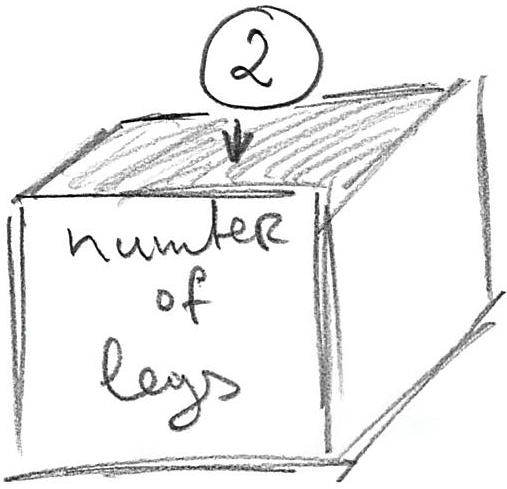
\includegraphics[width=0.5\linewidth]{images/variable-as-box} \end{center}

In Python würdest du schreiben

\begin{Shaded}
\begin{Highlighting}[]
\NormalTok{anzahl\_der\_beine }\OperatorTok{=} \DecValTok{2}
\end{Highlighting}
\end{Shaded}

Die obige \textbf{Zuweisungsanweisung} hat eine sehr einfache Struktur:

\begin{Shaded}
\begin{Highlighting}[]
\OperatorTok{\textless{}}\NormalTok{variablen}\OperatorTok{{-}}\NormalTok{name}\OperatorTok{\textgreater{}} \OperatorTok{=} \OperatorTok{\textless{}}\NormalTok{wert}\OperatorTok{\textgreater{}}
\end{Highlighting}
\end{Shaded}

Der Variablenname (das Namensschild auf der Kiste) sollte aussagekräftig sein, er kann mit Buchstaben oder \_ beginnen und kann Buchstaben, Zahlen und das Symbol \_ enthalten, aber keine Leerzeichen, Tabs, Sonderzeichen usw. Python empfiehlt\footnote{Naja, eigentlich \href{https://www.python.org/dev/peps/pep-0008/}{besteht} es darauf.} dass du die \textbf{snake\_case} Schreibweise (alles in Kleinbuchstaben, Unterstrich für Leerzeichen) verwendest, um deine Variablennamen zu formatieren. Der \texttt{\textless{}Wert\textgreater{}} auf der rechten Seite ist eine komplexere Geschichte, da er fest codiert sein kann (wie im obigen Beispiel), berechnet werden kann, indem andere Variablen oder dieselbe Variable, zurückgegeben von einer Funktion, usw. verwendet werden.

Die Verwendung von Variablen bedeutet, dass du dich auf die \textbf{Bedeutung} der entsprechenden Werte konzentrieren kannst, anstatt dir Sorgen darüber zu machen, was diese Werte sind. Beispielsweise kannst du das nächste Mal, wenn du etwas auf Grundlage der Anzahl der Beine eines Charakters berechnen musst (z.B., wie viele Paar Schuhe benötigt ein Charakter), dies auf Grundlage des aktuellen Wertes der Variablen \texttt{anzahl\_der\_beine} berechnen, anstatt anzunehmen, dass es \texttt{1} ist.

\begin{Shaded}
\begin{Highlighting}[]
\CommentTok{\# SCHLECHT: Warum 1? Ist es, weil der Character zwei Beine hat oder}
\CommentTok{\# weil wir jedem Character ein Paar Schuhe geben, unabhängig von}
\CommentTok{\# seiner tatsächlichen Anzahl von Beinen?}
\NormalTok{paar\_schuhe }\OperatorTok{=} \DecValTok{1}

\CommentTok{\# BESSER (aber was, wenn unser Charakter nur ein Bein hat?)}
\NormalTok{paar\_schuhe }\OperatorTok{=}\NormalTok{ anzahl\_der\_beine }\OperatorTok{/} \DecValTok{2}
\end{Highlighting}
\end{Shaded}

Variablen geben dir auch Flexibilität. Ihre Werte können sich während des Programmablaufs ändern: Der Punktestand des Spielers steigt, die Anzahl der Leben nimmt ab, die Anzahl der Zauber, die er wirken kann, steigt oder fällt je nach ihrem Einsatz, usw. Dennoch kannst du immer den Wert in der Variablen verwenden, um die notwendigen Berechnungen durchzuführen. Hier ist zum Beispiel ein leicht erweitertes Beispiel für \texttt{anzahl\_der\_schuhe}.

\begin{Shaded}
\begin{Highlighting}[]
\NormalTok{anzahl\_der\_beine }\OperatorTok{=} \DecValTok{2}

\CommentTok{\# ...}
\CommentTok{\# etwas passiert und unser Charakter wird in einen Tintenfisch verwandelt}
\NormalTok{anzahl\_der\_beine }\OperatorTok{=} \DecValTok{8}
\CommentTok{\# ...}

\CommentTok{\# der gleiche Code funktioniert immer noch und wir können immer noch die richtige Anzahl an Schuhpaaren berechnen}
\NormalTok{paar\_schuhe }\OperatorTok{=}\NormalTok{ anzahl\_der\_beine }\OperatorTok{/} \DecValTok{2}
\end{Highlighting}
\end{Shaded}

Wie bereits erwähnt, kannst du eine Variable als eine beschriftete Kiste betrachten, in die du etwas hineinlegen kannst. Das bedeutet, dass du immer den alten Wert ``wegwerfen'' und etwas Neues hineinlegen kannst. Im Falle von Variablen geschieht der ``Wegwerf''-Teil automatisch, da ein neuer Wert den alten überschreibt. Überprüfe selbst, welcher der endgültige Wert der Variable im unten stehenden Code ist?

\begin{Shaded}
\begin{Highlighting}[]
\NormalTok{anzahl\_der\_beine }\OperatorTok{=} \DecValTok{2}
\NormalTok{anzahl\_der\_beine }\OperatorTok{=} \DecValTok{5}
\NormalTok{anzahl\_der\_beine }\OperatorTok{=} \DecValTok{1}
\NormalTok{anzahl\_der\_beine}
\end{Highlighting}
\end{Shaded}

Mache Übung \#1.

Beachte, dass eine Variable (eine ``Kiste mit Namensschild'') erst existiert, nachdem du ihr etwas zugewiesen hast. Der folgende Code erzeugt also einen \texttt{NameError}, die Python-art zu sagen, dass sie noch nie von der Variable \texttt{anzahl\_der\_haende} gehört hat.

\begin{Shaded}
\begin{Highlighting}[]
\NormalTok{anzahl\_der\_beine }\OperatorTok{=} \DecValTok{2}
\NormalTok{anzahl\_der\_handschuhe }\OperatorTok{=}\NormalTok{ anzahl\_der\_haende }\OperatorTok{/} \DecValTok{2}
\end{Highlighting}
\end{Shaded}

Du kannst jedoch eine Variable erstellen, die keinen \emph{spezifischen} Wert hat, indem du ihr \texttt{None} zuweist. \texttt{None} wurde speziell für die Bedeutung \emph{kein Wert} oder \emph{nichts} zur Sprache hinzugefügt.

\begin{Shaded}
\begin{Highlighting}[]
\NormalTok{anzahl\_der\_haende }\OperatorTok{=} \VariableTok{None} \CommentTok{\# Die Variable existiert jetzt, hat aber keinen speziellen Wert.}
\end{Highlighting}
\end{Shaded}

Wie du bereits gesehen hast, kannst du einen Wert \emph{berechnen}, anstatt ihn anzugeben. Was wäre die Antwort hier?

\begin{Shaded}
\begin{Highlighting}[]
\NormalTok{anzahl\_der\_beine }\OperatorTok{=} \DecValTok{2} \OperatorTok{*} \DecValTok{2}
\NormalTok{anzahl\_der\_beine }\OperatorTok{=} \DecValTok{7} \OperatorTok{{-}} \DecValTok{2}
\NormalTok{anzahl\_der\_beine}
\end{Highlighting}
\end{Shaded}

Mache Übung \#2.

\hypertarget{zuweisungen-sind-keine-gleichungen}{%
\section{Zuweisungen sind keine Gleichungen!}\label{zuweisungen-sind-keine-gleichungen}}

\textbf{Sehr wichtig}: obwohl Zuweisungen \emph{wie} mathematische Gleichungen \emph{aussehen}, sind sie \textbf{keine Gleichungen!} Sie folgen einer \textbf{sehr wichtigen} Regel, die Sie im Kopf behalten müssen, wenn Sie Zuweisungen verstehen: die rechte Seite eines Ausdrucks wird \emph{zuerst} ausgewertet, bis der Endwert berechnet ist. Erst dann wird dieser Endwert der auf der linken Seite angegebenen Variable zugewiesen (also in die Kiste gelegt). Das bedeutet, dass Sie die gleiche Variable auf \emph{beiden} Seiten verwenden können! Sehen wir uns diesen Code an:

\begin{Shaded}
\begin{Highlighting}[]
\NormalTok{x }\OperatorTok{=} \DecValTok{2}
\NormalTok{y }\OperatorTok{=} \DecValTok{5}
\NormalTok{x }\OperatorTok{=}\NormalTok{ x }\OperatorTok{+}\NormalTok{ y }\OperatorTok{{-}} \DecValTok{4}
\end{Highlighting}
\end{Shaded}

Was passiert, wenn der Computer die letzte Zeile auswertet? Zunächst nimmt er die \emph{aktuellen} Werte aller Variablen (\texttt{2} für \texttt{x} und \texttt{5} für \texttt{y}) und setzt sie in den Ausdruck. Nach diesem internen Schritt sieht der Ausdruck so aus:

\begin{Shaded}
\begin{Highlighting}[]
\NormalTok{x }\OperatorTok{=} \DecValTok{2} \OperatorTok{+} \DecValTok{5} \OperatorTok{{-}} \DecValTok{4}
\end{Highlighting}
\end{Shaded}

Dann berechnet er den Ausdruck auf der rechten Seite und speichert, \textbf{sobald die Berechnung abgeschlossen ist}, diesen neuen Wert in \texttt{x}

\begin{Shaded}
\begin{Highlighting}[]
\NormalTok{x }\OperatorTok{=} \DecValTok{3}
\end{Highlighting}
\end{Shaded}

Machen Sie die Übung \#3, um sicherzugehen, dass Sie dies verstanden haben.

\hypertarget{constants}{%
\section{Konstanten}\label{constants}}

Obwohl die eigentliche Stärke von Variablen darin besteht, dass Sie ihren Wert ändern können, sollten Sie sie auch dann verwenden, wenn der Wert im gesamten Programm konstant bleibt. In Python gibt es keine echten Konstanten, sondern die Übereinkunft, dass ihre Namen vollständig \texttt{GROSSGESCHRIEBEN} sein sollten. Entsprechend wissen Sie, wenn Sie \texttt{SOLCH\_EINE\_VARIABLE} sehen, dass Sie ihren Wert nicht ändern sollten. Technisch gesehen ist das nur eine Empfehlung, denn niemand kann Sie davon abhalten, den Wert einer \texttt{KONSTANTE} zu ändern. Aber ein großer Teil der Benutzerfreundlichkeit von Python resultiert aus solchen Übereinkünften (wie der \texttt{snake\_case} Konvention oben). Wir werden später mehr von solchen Übereinkünften treffen, zum Beispiel beim Lernen über Objekte.

Unter Berücksichtigung all dessen, wenn die Anzahl der Beine im Spiel konstant bleibt, sollten Sie diese Konstanz betonen und schreiben

\begin{Shaded}
\begin{Highlighting}[]
\NormalTok{ANZAHL\_DER\_BEINE }\OperatorTok{=} \DecValTok{2}
\end{Highlighting}
\end{Shaded}

Ich empfehle dringend die Verwendung von Konstanten und vermeide das Hardcoding von Werten. Erstens, wenn Sie mehrere identische Werte haben, die verschiedene Dinge bedeuten (2 Beine, 2 Augen, 2 Ohren, 2 Fahrzeuge pro Figur, etc.), wird Ihnen eine \texttt{2} im Code nicht verraten, was diese \texttt{2} bedeutet (die Beine? Die Ohren? Der Punktemultiplikator?). Sie können das natürlich herausfinden, basierend auf dem Code, der diese Nummer verwendet, aber Sie könnten sich diese zusätzliche Mühe ersparen und stattdessen eine ordnungsgemäß benannte Konstante verwenden. Dann lesen Sie einfach ihren Namen und die Bedeutung des Wertes wird offensichtlich, und es ist die Bedeutung und nicht der tatsächliche Wert, der Sie hauptsächlich interessiert. Zweitens, wenn Sie entscheiden, diesen Wert dauerhaft zu \emph{ändern} (sagen wir, unsere Hauptfigur ist jetzt ein Dreifuß), bedeutet die Verwendung einer Konstante, dass Sie sich nur an einer Stelle Sorgen machen müssen, der Rest des Codes bleibt unverändert. Wenn Sie diese Zahl hart codiert haben, erwartet Sie eine aufregende \footnote{nicht wirklich} und definitiv lange Suche und Ersetzung im gesamten Code.

Machen Sie die Übung \#4.

\hypertarget{value-types}{%
\section{Datentypen}\label{value-types}}

Bisher haben wir nur ganzzahlige numerische Werte verwendet (1, 2, 5, 1000\ldots). Obwohl Python \href{https://docs.python.org/3/library/stdtypes.html}{viele verschiedene Datentypen} unterstützt, konzentrieren wir uns zunächst auf eine kleine Auswahl davon:

\begin{itemize}
\tightlist
\item
  Ganze Zahlen, die wir bereits verwendet haben, z.B. \texttt{-1}, \texttt{100000}, \texttt{42}.
\item
  Fließkommazahlen, die jeden realen Wert annehmen können, z.B. \texttt{42.0}, \texttt{3.14159265359}, \texttt{2.71828}.
\item
  Zeichenketten, die Text speichern können. Der Text ist zwischen entweder gepaarten Anführungszeichen \texttt{"einiger\ Text"} oder Apostrophen \texttt{\textquotesingle{}einiger\ Text\textquotesingle{}} eingeschlossen. Das bedeutet, dass Sie Anführungszeichen oder Apostrophe innerhalb der Zeichenkette verwenden können, solange sie von der Alternative umschlossen ist. Z.B., \texttt{"Schüleraufgaben"} (eingeschlossen in \texttt{"}, Apostroph \texttt{\textquotesingle{}} innen) oder \texttt{\textquotesingle{}"Alle\ Verallgemeinerungen\ sind\ falsch,\ auch\ diese."\ Mark\ Twain\textquotesingle{}} (Zitat von Apostrophen eingeschlossen). Es gibt noch viel mehr zu Zeichenketten und wir werden dieses Material im Laufe des Kurses behandeln.
\item
  Logische / boolesche Werte, die entweder \texttt{True} oder \texttt{False} sind.
\end{itemize}

Bei der Verwendung einer Variable ist es wichtig, dass Sie wissen, welchen Datentyp sie speichert, und das liegt meist bei Ihnen. In einigen Fällen wird Python einen Fehler ausgeben, wenn Sie versuchen, eine Rechnung mit inkompatiblen Datentypen durchzuführen. In anderen Fällen wird Python Werte automatisch zwischen bestimmten Typen konvertieren, z.B. ist jeder Ganzzahlwert auch ein Realwert, so dass die Konvertierung von \texttt{1} zu \texttt{1.0} meist trivial und automatisch ist. In anderen Fällen müssen Sie jedoch möglicherweise eine explizite Konvertierung verwenden. Gehen Sie zur Übung \#5 und versuchen Sie zu erraten, welcher Code laufen wird und welcher einen Fehler wegen inkompatiblen Typen werfen wird?

\begin{Shaded}
\begin{Highlighting}[]
\DecValTok{5} \OperatorTok{+} \FloatTok{2.0}
\CommentTok{\textquotesingle{}5\textquotesingle{}} \OperatorTok{+} \DecValTok{2}
\CommentTok{\textquotesingle{}5\textquotesingle{}} \OperatorTok{+} \StringTok{\textquotesingle{}2\textquotesingle{}}
\CommentTok{\textquotesingle{}5\textquotesingle{}} \OperatorTok{+} \VariableTok{True}
\DecValTok{5} \OperatorTok{+} \VariableTok{True}
\end{Highlighting}
\end{Shaded}

Mache Übung \#5.

Überrascht vom letzten? Das liegt daran, dass intern \texttt{True} auch \texttt{1} und \texttt{False} \texttt{0} ist!

Sie können explizit von einem Typ in einen anderen umwandeln, indem Sie spezielle Funktionen verwenden. Beispielsweise können Sie eine Zahl oder einen logischen Wert in einen String umwandeln, indem Sie einfach \href{https://docs.python.org/3/library/functions.html\#func-str}{str(\textless value\textgreater)} schreiben. Was wäre das Ergebnis in den untenstehenden Beispielen?

\begin{Shaded}
\begin{Highlighting}[]
\BuiltInTok{str}\NormalTok{(}\DecValTok{10} \OperatorTok{/} \DecValTok{2}\NormalTok{)}
\BuiltInTok{str}\NormalTok{(}\FloatTok{2.5} \OperatorTok{+} \VariableTok{True}\NormalTok{)}
\BuiltInTok{str}\NormalTok{(}\VariableTok{True}\NormalTok{)}
\end{Highlighting}
\end{Shaded}

Mache Übung \#6.

Ähnlich können Sie mit der Funktion \href{https://docs.python.org/3/library/functions.html\#bool}{bool(\textless value\textgreater)} in eine logische/boolesche Variable umwandeln. Die Regeln sind einfach, für numerische Werte ist \texttt{0} gleich \texttt{False}, jeder andere Nicht-Null-Wert wird in \texttt{True} umgewandelt. Für Zeichenketten wird eine leere Zeichenkette \texttt{\textquotesingle{}\textquotesingle{}} als \texttt{False} bewertet und eine nicht leere Zeichenkette wird in \texttt{True} umgewandelt. Was wäre die Ausgabe in den untenstehenden Beispielen?

\begin{Shaded}
\begin{Highlighting}[]
\BuiltInTok{bool}\NormalTok{(}\OperatorTok{{-}}\DecValTok{10}\NormalTok{)}
\BuiltInTok{bool}\NormalTok{(}\FloatTok{0.0}\NormalTok{)}

\NormalTok{secret\_message }\OperatorTok{=} \StringTok{\textquotesingle{}\textquotesingle{}}
\BuiltInTok{bool}\NormalTok{(secret\_message)}

\BuiltInTok{bool}\NormalTok{(}\StringTok{\textquotesingle{}False\textquotesingle{}}\NormalTok{)}
\end{Highlighting}
\end{Shaded}

Mache Übung \#7.

Die Umwandlung in Ganzzahlen oder Fließkommazahlen mit \href{https://docs.python.org/3/library/functions.html\#int}{int(\textless value\textgreater)} bzw. \href{https://docs.python.org/3/library/functions.html\#float}{float(\textless value\textgreater)} ist komplizierter. Der einfachste Fall ist von logisch auf Ganzzahl/Fließkommazahl, da \texttt{True} Ihnen \texttt{int(True)} ist \texttt{1} und \texttt{float(True)} ist \texttt{1.0} gibt und \texttt{False} gibt Ihnen \texttt{0}/\texttt{0.0}. Beim Umwandeln von Fließkommazahl auf Ganzzahl lässt Python einfach den Bruchteilteil fallen (es rundet nicht richtig!). Bei der Umwandlung einer Zeichenkette muss es sich um eine gültige Zahl des entsprechenden Typs handeln, sonst wird ein Fehler erzeugt. Sie können z. B. eine Zeichenkette wie \texttt{"123"} in eine Ganzzahl oder eine Fließkommazahl umwandeln, aber das funktioniert nicht für \texttt{"a123"}. Darüber hinaus können Sie \texttt{"123.4"} in eine Fließkommazahl umwandeln, aber nicht in eine Ganzzahl, da sie einen Bruchteil enthält. Angesichts all dessen, welche Zellen würden funktionieren und welche Ausgabe würden sie erzeugen?

\begin{Shaded}
\begin{Highlighting}[]
\BuiltInTok{float}\NormalTok{(}\VariableTok{False}\NormalTok{)}
\BuiltInTok{int}\NormalTok{(}\OperatorTok{{-}}\FloatTok{3.3}\NormalTok{)}
\BuiltInTok{float}\NormalTok{(}\StringTok{"67.8"}\NormalTok{)}
\BuiltInTok{int}\NormalTok{(}\StringTok{"123+3"}\NormalTok{)}
\end{Highlighting}
\end{Shaded}

Mache Übung \#8.

\hypertarget{print}{%
\section{Ausgabe drucken}\label{print}}

Um den Wert auszudrucken, müssen Sie die Funktion \href{https://docs.python.org/3/library/functions.html\#print}{print()} verwenden (wir werden später allgemein über Funktionen sprechen). Im einfachsten Fall übergeben Sie den Wert und er wird ausgegeben.

\begin{Shaded}
\begin{Highlighting}[]
\BuiltInTok{print}\NormalTok{(}\DecValTok{5}\NormalTok{)}
\CommentTok{\#\textgreater{} 5}
\end{Highlighting}
\end{Shaded}

oder

\begin{Shaded}
\begin{Highlighting}[]
\BuiltInTok{print}\NormalTok{(}\StringTok{"fünf"}\NormalTok{)}
\CommentTok{\#\textgreater{} fünf}
\end{Highlighting}
\end{Shaded}

Natürlich wissen Sie bereits über die Variablen Bescheid, also statt den Wert direkt einzugeben, können Sie stattdessen eine Variable übergeben und ihr \emph{Wert} wird ausgegeben.

\begin{Shaded}
\begin{Highlighting}[]
\NormalTok{anzahl\_der\_pfannkuchen }\OperatorTok{=} \DecValTok{10}
\BuiltInTok{print}\NormalTok{(anzahl\_der\_pfannkuchen)}
\CommentTok{\#\textgreater{} 10}
\end{Highlighting}
\end{Shaded}

oder

\begin{Shaded}
\begin{Highlighting}[]
\NormalTok{frühstück }\OperatorTok{=} \StringTok{"pfannkuchen"}
\BuiltInTok{print}\NormalTok{(frühstück)}
\CommentTok{\#\textgreater{} pfannkuchen}
\end{Highlighting}
\end{Shaded}

Sie können auch mehr als einen Wert/Variablen an die Druckfunktion übergeben und alle Werte werden nacheinander gedruckt. Wenn wir dem Benutzer zum Beispiel sagen wollen, was ich zum Frühstück hatte, können wir das tun

\begin{Shaded}
\begin{Highlighting}[]
\NormalTok{frühstück }\OperatorTok{=} \StringTok{"pfannkuchen"}
\NormalTok{anzahl\_der\_artikel }\OperatorTok{=} \DecValTok{10}
\BuiltInTok{print}\NormalTok{(frühstück, anzahl\_der\_artikel)}
\CommentTok{\#\textgreater{} pfannkuchen 10}
\end{Highlighting}
\end{Shaded}

Was wird von dem untenstehenden Code gedruckt?

\begin{Shaded}
\begin{Highlighting}[]
\NormalTok{abendessen }\OperatorTok{=} \StringTok{"steak"}
\NormalTok{zähler }\OperatorTok{=} \DecValTok{4}
\NormalTok{nachtisch }\OperatorTok{=} \StringTok{"muffins"}

\BuiltInTok{print}\NormalTok{(zähler, abendessen, zähler, nachtisch)}
\end{Highlighting}
\end{Shaded}

Mache Übung \#9.

Allerdings möchten Sie wahrscheinlich expliziter sein, wenn Sie die Informationen ausdrucken. Stellen Sie sich zum Beispiel vor, Sie haben diese drei Variablen:

\begin{Shaded}
\begin{Highlighting}[]
\NormalTok{mahlzeit }\OperatorTok{=} \StringTok{"Frühstück"}
\NormalTok{gericht }\OperatorTok{=} \StringTok{"Pfannkuchen"}
\NormalTok{anzahl }\OperatorTok{=} \DecValTok{10}
\end{Highlighting}
\end{Shaded}

Sie könnten natürlich \texttt{print(mahlzeit,\ gericht,\ anzahl)} machen, aber es wäre schöner, ``\emph{Ich hatte \textbf{10 Pfannkuchen} zum \textbf{Frühstück}}'' zu drucken, wobei die in Fettschrift gedruckten Elemente die eingefügten Variablenwerte wären. Dafür müssen wir die Formatierung von Zeichenketten verwenden. Bitte beachten Sie, dass die Formatierung von Zeichenketten nicht spezifisch für das Drucken ist, Sie können einen neuen Zeichenkettenwert über die Formatierung erstellen und ihn in einer Variable speichern, ohne ihn auszudrucken, oder ihn ausdrucken, ohne ihn zu speichern.

\hypertarget{string-formatting}{%
\section{Formatierung von Zeichenketten}\label{string-formatting}}

Eine großartige Ressource zur Formatierung von Zeichenketten in Python ist \href{https://pyformat.info/}{pyformat.info}. Da sich Python ständig weiterentwickelt, gibt es nun mehr als eine Art, Zeichenketten zu formatieren. Im Folgenden werde ich das ``alte'' Format vorstellen, das auf der klassischen Formatierung von Zeichenketten basiert, die in der Funktion \texttt{sprintf} in C, Matlab, R und vielen anderen Programmiersprachen verwendet wird. Es ist etwas weniger flexibel als neuere, aber für einfache Aufgaben ist der Unterschied vernachlässigbar. Das Wissen über das alte Format ist nützlich wegen seiner Allgemeinheit. Wenn Sie Alternativen lernen möchten, lesen Sie unter dem oben angegebenen Link.

Der allgemeine Aufruf lautet \texttt{"ein\ String\ mit\ Formatierung"\%(Tupel\ von\ Werten,\ die\ während\ der\ Formatierung\ verwendet\ werden)}. Sie werden später mehr über Tupel lernen. Gehen Sie im Moment davon aus, dass es sich einfach um eine durch Kommas getrennte Liste von Werten handelt, die in runden Klammern eingeschlossen sind: \texttt{(1,\ 2,\ 3)}.

In \texttt{"ein\ String\ mit\ Formatierung"}, geben Sie an, wo Sie den Wert mit dem Zeichen \texttt{\%} einfügen möchten, das von einer \emph{optionalen} Formatierungsinformation und dem \emph{erforderlichen} Symbol, das den \textbf{Typ} des Wertes definiert, gefolgt wird. Die Typsymbole sind

\begin{itemize}
\tightlist
\item
  \texttt{s} für Zeichenkette
\item
  \texttt{d} für eine Ganzzahl
\item
  \texttt{f} für einen Fließkommawert
\item
  \texttt{g} für einen ``optimal'' gedruckten Fließkommawert, so dass für große Werte die wissenschaftliche Notation verwendet wird (\emph{z.B.}, \texttt{10e5} statt \texttt{100000}).
\end{itemize}

Hier ist ein Beispiel, wie man einen String mit einer Ganzzahl formatiert:

\begin{Shaded}
\begin{Highlighting}[]
\BuiltInTok{print}\NormalTok{(}\StringTok{"Ich hatte }\SpecialCharTok{\%d}\StringTok{ Pfannkuchen zum Frühstück"}\OperatorTok{\%}\NormalTok{(}\DecValTok{10}\NormalTok{))}
\CommentTok{\#\textgreater{} Ich hatte 10 Pfannkuchen zum Frühstück}
\end{Highlighting}
\end{Shaded}

Sie sind nicht darauf beschränkt, einen einzigen Wert in einen String einzufügen. Sie können weitere Positionen über \texttt{\%} angeben, müssen jedoch sicherstellen, dass Sie die richtige Anzahl von Werten in der richtigen Reihenfolge übergeben. Können Sie vor dem Ausführen herausfinden, welcher Aufruf tatsächlich funktioniert (und was die Ausgabe sein wird) und welcher einen Fehler verursacht?

\begin{Shaded}
\begin{Highlighting}[]
\BuiltInTok{print}\NormalTok{(}\StringTok{\textquotesingle{}Ich hatte }\SpecialCharTok{\%d}\StringTok{ Pfannkuchen und entweder }\SpecialCharTok{\%d}\StringTok{ oder }\SpecialCharTok{\%d}\StringTok{ Steaks zum Abendessen\textquotesingle{}}\OperatorTok{\%}\NormalTok{(}\DecValTok{2}\NormalTok{))}
\BuiltInTok{print}\NormalTok{(}\StringTok{\textquotesingle{}Ich hatte }\SpecialCharTok{\%d}\StringTok{ Pfannkuchen und }\SpecialCharTok{\%d}\StringTok{ Steaks zum Abendessen\textquotesingle{}}\OperatorTok{\%}\NormalTok{(}\DecValTok{7}\NormalTok{, }\DecValTok{10}\NormalTok{))}
\BuiltInTok{print}\NormalTok{(}\StringTok{\textquotesingle{}Ich hatte }\SpecialCharTok{\%d}\StringTok{ Pfannkuchen und }\SpecialCharTok{\%d}\StringTok{ Steaks zum Abendessen\textquotesingle{}}\OperatorTok{\%}\NormalTok{(}\DecValTok{1}\NormalTok{, }\DecValTok{7}\NormalTok{, }\DecValTok{10}\NormalTok{))}
\end{Highlighting}
\end{Shaded}

Machen Sie Übung \#10.

Wie oben erwähnt, haben Sie im Falle von echten Werten zwei Möglichkeiten: \texttt{\%f} und \texttt{\%g}. Letzterer verwendet die wissenschaftliche Notation (z.B. \texttt{1e10} für \texttt{10000000000}), um eine Darstellung kompakter zu machen.

Machen Sie Übung \#11, um ein besseres Gefühl für den Unterschied zu bekommen.

Es gibt noch viel mehr zur Formatierung und Sie können auf \href{https://pyformat.info/}{pyformat.info} darüber lesen. Diese Grundlagen sind jedoch ausreichend, um in dem nächsten Kapitel mit der Programmierung unseres ersten Spiels zu beginnen.

\hypertarget{guess-the-number-single-round}{%
\chapter{Errate die Zahl: eine einzelne Runden Edition}\label{guess-the-number-single-round}}

Das vorherige Kapitel deckte die Grundlagen von Python ab, sodass Du nun bereit bist, Dein erstes Spiel zu entwickeln! Wir werden es Schritt für Schritt aufbauen, da es viel zu lernen gibt über Eingaben, Bibliotheken, bedingte Aussagen und Einrückungen.

Bevor Du anfängst, erstelle einen neuen Ordner (innerhalb Deines \protect\hyperlink{files-folder}{Kursordners}), benenne ihn zum Beispiel ``guess-the-number'', lade das \href{notebooks/Guess\%20the\%20number\%20-\%20single\%20round.ipynb}{Übungsnotizbuch} herunter, kopiere es in den neu erstellten Ordner und öffne es in \protect\hyperlink{jupyter-notebooks}{Jupyter Notebook}. Wie im vorherigen Kapitel wird es Übungen zum Lesen und Verstehen des Codes enthalten.

Wir werden jedoch \protect\hyperlink{install-vs-code}{VS Code} verwenden, um Skripte mit dem eigentlichen Spiel zu programmieren. Du musst für jede Code-Praxis eine separate Datei erstellen\footnote{Du kannst den vorherigen Code ``Speichern unter\ldots{}'' um das Herumkopieren von Dingen per Hand zu vermeiden.} (z.B., \emph{code01.py}\footnote{Ich empfehle die Verwendung von \texttt{01} statt von \texttt{1}, da dies eine konsistente Dateisortierung in Deinem Dateimanager gewährleistet}, \emph{code02.py}, etc.) Dies ist nicht die effizienteste Implementierung einer Versionskontrolle und wird sicherlich den Ordner überladen. Aber es würde mir ermöglichen, Deine Lösungen für jeden Schritt zu sehen, was es mir leichter machen würde, Feedback zu geben. Zum Einreichen der Aufgabe, zippe einfach den Ordner und reiche die Zip-Datei ein.

\hypertarget{konzepte-des-kapitels-1}{%
\section{Konzepte des Kapitels}\label{konzepte-des-kapitels-1}}

\begin{itemize}
\tightlist
\item
  \protect\hyperlink{documenting-your-code}{Dokumentation des Codes}.
\item
  \protect\hyperlink{debugging}{Debuggen von Code}.
\item
  Eingabe einer \protect\hyperlink{input-function}{Eingabe} von einem Benutzer.
\item
  Verwendung von \protect\hyperlink{comparisons}{Vergleichen} in \protect\hyperlink{if-statement}{bedingten Aussagen}.
\item
  Verwendung von \protect\hyperlink{indentation}{Einrückungen}, um Aussagen zu gruppieren.
\item
  Verwendung von Python \protect\hyperlink{using-libraries}{Bibliotheken}.
\item
  Generieren von \protect\hyperlink{picking-a-number-randomly}{Zufallszahlen}.
\end{itemize}

\hypertarget{das-spiel}{%
\section{Das Spiel}\label{das-spiel}}

Wir werden ein Spiel programmieren, bei dem ein Teilnehmer (Computer) eine Zahl innerhalb eines bestimmten Bereichs auswählt (sagen wir, zwischen 1 und 10) und der andere Teilnehmer (menschlicher Spieler) versucht, diese zu erraten. Nach jedem Versuch des Menschen antwortet der Computer, ob die tatsächliche Zahl niedriger als die Vermutung ist, höher als die Vermutung ist oder mit ihr übereinstimmt. Das Spiel ist vorbei, wenn der Spieler die Zahl richtig errät oder (in der späteren Version des Spiels) keine Versuche mehr hat.

Unsere erste Version wird nur einen Versuch zulassen und der Gesamtspielalgorithmus wird folgendermaßen aussehen:

\begin{enumerate}
\def\labelenumi{\arabic{enumi}.}
\tightlist
\item
  der Computer generiert eine Zufallszahl zwischen 1 und 10
\item
  druckt sie aus für Debugging-Zwecke
\item
  fordert den Benutzer auf, eine Vermutung einzugeben
\item
  vergleicht die beiden Zahlen und gibt das Ergebnis aus: ``Meine Zahl ist niedriger'', ``Meine Zahl ist höher'' oder ``Genau richtig!''
\end{enumerate}

\hypertarget{lass-uns-eine-zahl-auswuxe4hlen}{%
\section{Lass uns eine Zahl auswählen}\label{lass-uns-eine-zahl-auswuxe4hlen}}

Beginnen wir damit, nur die ersten zwei Schritte des Programms zu implementieren. Erstelle zuerst eine Variable, die eine Zahl enthält, die der Computer ``ausgesucht'' hat. Wir nennen sie \texttt{number\_picked} (Du kannst auch einen anderen aussagekräftigen Namen verwenden, aber es könnte einfacher sein, wenn wir alle den gleichen Namen verwenden). Um die Dinge am Anfang einfacher zu machen, codieren wir eine beliebige Zahl zwischen 1 und 10 hart (wähle die, die Dir gefällt). Dann lass uns diese ausdrucken, so dass wir die Zahl selbst kennen\footnote{Natürlich wissen wir es, weil wir es hart kodiert haben, aber das wird nicht der Fall sein, wenn der Computer es zufällig generiert, also lassen wir uns für die Zukunft planen}. Verwende die Zeichenkettenformatierung, um die Dinge benutzerfreundlich zu gestalten, z. B. drucke etwas aus wie ``Die Zahl, die ich ausgewählt habe, ist \ldots{}''. Du solltest in der Lage sein, dies mit dem Wissen aus dem \protect\hyperlink{string-formatting}{vorherigen Kapitel} zu tun. Dein Code sollte aus zwei Zeilen bestehen:

\begin{Shaded}
\begin{Highlighting}[]
\CommentTok{\# 1. erstelle Variable und setze ihren Wert}
\CommentTok{\# 2. gebe den Wert aus}
\end{Highlighting}
\end{Shaded}

Probiere diesen Zweizeiler in einem Jupyter Notebook aus (erstelle ein leeres Notebook nur dafür). Wenn Du damit zufrieden bist, kopiere-den Code in \texttt{code01.py} und lies weiter, um zu erfahren, wie Du es dokumentieren und ausführen kannst.

Füge Deinen Code in \texttt{code01.py} ein.

\hypertarget{dokumentiere-deinen-code-1}{%
\section{Dokumentiere Deinen Code}\label{dokumentiere-deinen-code-1}}

Jetzt, wo Du Deine erste Datei mit einem Python-Programm hast, solltest Du es dokumentieren. Die Dokumentation eines zwei Zeilen langen und einfachen Programms mag albern erscheinen, aber es sollte etwas Automatisches sein. Später wirst Du mehrere Zeilen Kommentare verwenden, um eine einzelne Zeilenfunktion zu dokumentieren. Noch einmal, es geht nicht um den Code, der funktioniert, es geht um den Code, den Du verstehen kannst. In gewisser Weise ist es besser, ein sauberes, gut dokumentiertes Programm zu haben, das momentan nicht korrekt funktioniert, als einen undokumentierten Spaghetti-Code, der funktioniert. Du kannst das Erstere korrigieren und aktualisieren, das Letztere zu warten oder zu aktualisieren\ldots{}

In Python hast Du zwei Möglichkeiten, Kommentare zu schreiben: mehrzeilig und einzeilig

\begin{Shaded}
\begin{Highlighting}[]
\CommentTok{\textquotesingle{}\textquotesingle{}\textquotesingle{}Ein }
\CommentTok{mehrzeiliger }
\CommentTok{Kommentar}
\CommentTok{\textquotesingle{}\textquotesingle{}\textquotesingle{}}

\CommentTok{\#  Ein einzeiliger Kommentar.}
\end{Highlighting}
\end{Shaded}

Verwende mehrzeilige Kommentare, um die Dokumentation für einzelne Dateien, Funktionen, Klassen, Methoden usw. zu schreiben. Du wirst lernen, wie Du diese Dokumentation im Numpy-Docstring-Stil formatierst, sobald Du Funktionen kennst. In unserem Fall solltest Du Deine \texttt{code01.py}-Datei mit einem mehrzeiligen Kommentar beginnen, der kurz beschreibt, welches Programm sie enthält. Mindestens solltest Du schreiben, dass dies ein \emph{Guess a Number}-Spiel ist. Wahrscheinlich ist es eine gute Idee, zu skizzieren, worum es in dem Spiel geht.

Verwende einzeilige Kommentare, um zu erklären, was in einem bestimmten Codeblock passiert. Du musst nicht jede Zeile kommentieren und Du solltest den Code nicht in menschlicher Sprache replizieren. Ein Kommentar sollte darüber sein, \emph{was} passiert, nicht \emph{wie}. Du hast bereits einen Block Code, also dokumentiere ihn mit einem einzelnen Satz.

Dokumentiere die \texttt{code01.py}.

\hypertarget{debugging}{%
\section{Ausführen und Debuggen deines Spiels in VS Code}\label{debugging}}

Jetzt, da wir ein zwei Zeilen langes Programm haben, können wir es ausführen und schon anfangen zu lernen, wie man es debuggt. Ja, unser aktuelles Programm ist wahrscheinlich zu einfach, um ein tatsächliches Debugging zu benötigen, aber es ist auch einfach genug, um das Verständnis des Debuggings zu erleichtern. Und das Debuggen ist eine entscheidende Fähigkeit, die ein laufendes Programm von einer Blackbox in etwas transparentes und leichtes\footnote{Oder zumindest leichter.} zu verstehen verwandelt. Weiter unten werde ich beschreiben, wie man in VS Code debuggt, aber du könntest \href{https://code.visualstudio.com/docs/python/debugging}{ein offizielles Handbuch} zu Rate ziehen, falls sich in der Zwischenzeit etwas geändert hat.

Es gibt zwei Möglichkeiten, ein Python-Programm in VS Code auszuführen. Zuerst kannst Du den \emph{``Run Python File in Terminal''} Abspielknopf auf der rechten Seite verwenden. Dies führt dein Programm \emph{ohne} Debugger aus, so dass Du es nur für die tatsächlichen Läufe des finalisierten Codes verwenden solltest. Trotzdem kannst Du versuchen, es auszuführen und zu sehen, ob es das ausgibt, was es sollte.

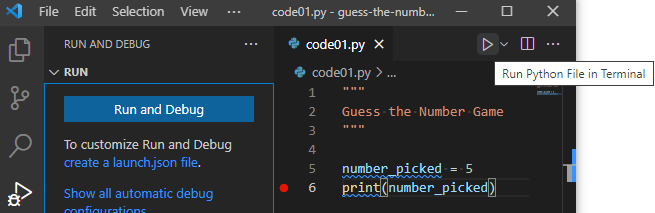
\includegraphics{images/debug-vs-run.png}
Die Alternative ist der Debugging-Reiter, der eine kleine Wanze auf dem Run-Knopf hat. Wenn Du ihn auswählst, wird \emph{``Run and Debug''} angezeigt. Klicke auf den Knopf und es werden verschiedene Optionen für verschiedene Arten von Python-Projekten und -Frameworks angeboten. Für unsere Absichten und Zwecke benötigen wir nur \emph{``Python File: Debug the currently active Python file''}. Klicke darauf und es wird Deinen Code ausführen (sollte genau so laufen wie mit dem anderen Knopf).

\begin{figure}
\centering
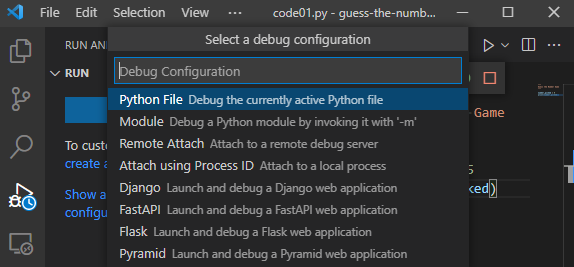
\includegraphics{images/debug-select-debug-configuration.png}
\caption{Selecting debugging configuration.}
\end{figure}

Du willst wahrscheinlich nicht die ganze Zeit durch Debugging-Tab → Run and Debug-Knopf → Konfiguration auswählen klicken. Ein besserer Weg ist es, es einmal für alle zu konfigurieren und dann die \textbf{F5}-Taste zu verwenden, um Deinen Code auszuführen. Klicke zunächst auf \emph{``Erstelle eine launch.json-Datei''} und wähle erneut \emph{``Python File: Debug the currently active Python file''} aus. Du wirst sehen, dass eine neue \emph{launch.json} Datei im Editor erscheint, die so aussehen sollte:

\begin{figure}
\centering
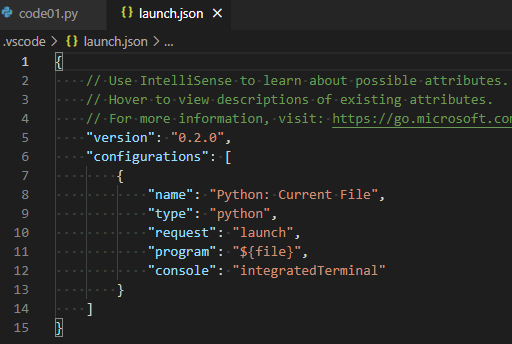
\includegraphics{images/debug-launch-json.png}
\caption{Debug configuration in launch.json file.}
\end{figure}

Das war's! VS Code hat für Dich eine Konfiguration erstellt. Jetzt kannst Du die \emph{launch.json}-Datei schließen und Dein Programm durch einfaches Drücken der \textbf{F5}-Taste ausführen. Versuch es! Wieder einmal sollte es genauso funktionieren wie zuvor, aber warum sind wir dann durch all diese Mühe gegangen? Weil der Debugger die Ausführung Deines Codes \emph{pausiert}, wann immer er auf ein Problem trifft und Dir die Chance gibt, Variablen zu untersuchen, Code-Snippets auszuführen usw. Im Gegensatz dazu wird das Ausführen der Python-Datei im Terminal (die erste Option) nur eine Fehlermeldung ausgeben und das Programm beenden. Außerdem kannst Du \emph{Breakpoints} verwenden, um das Programm an jeder Zeile anzuhalten, was Dir die Möglichkeit gibt, Deinen Code an jeder Stelle, die Du benötigst, zu untersuchen.

Du aktivierst Breakpoints, indem Du links von der Zeilennummer, die Dich interessiert, klickst. Hier habe ich auf Zeile 6 geklickt und Du kannst einen roten Punkt sehen, der einen aktiven Breakpoint anzeigt

\begin{figure}
\centering
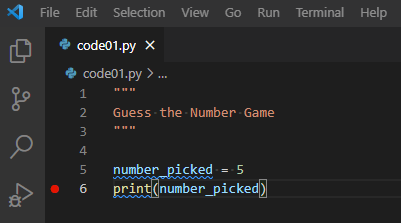
\includegraphics{images/debug-breakpoint.png}
\caption{Active breakpoint.}
\end{figure}

Wenn ich jetzt den Code über \textbf{F5} ausführe, hält das Programm an dieser Zeile \emph{bevor} es sie ausführt.

\begin{figure}
\centering
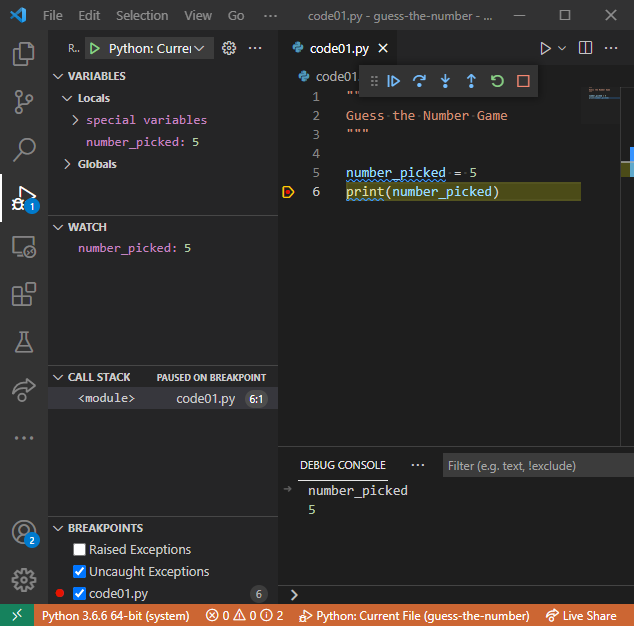
\includegraphics{images/debug-pause.png}
\caption{Program paused at the breakpoint.}
\end{figure}

Das gibt mir die Möglichkeit zu sehen, welchen Wert meine Variable \texttt{number\_picked} hat. Sie ist bereits in den lokalen Variablen aufgeführt (oben links). Aber ich habe sie auch zur Liste der beobachteten Variablen (\emph{Watch}, links in der Mitte) hinzugefügt und mir ihren Wert in der \emph{Debug Console} (unten) angesehen, die es mir ermöglicht, \emph{beliebigen} Python-Code auszuführen, während mein Programm angehalten ist. Mach das Gleiche und erkunde selbst diese unterschiedlichen Möglichkeiten. Sieh zum Beispiel, wie du \texttt{number\_picked\ +\ 1} oder \texttt{number\_picked\ *\ number\_picked} im \emph{Watch} Tab und in der \emph{Debug Console} berechnen kannst.

Sobald du fertig bist, den aktuellen Zustand des Programms zu untersuchen, hast du sechs Buttons oben zur Verfügung, um zu entscheiden, was als nächstes zu tun ist (fahre mit der Maus darüber, um Hinweise zu sehen). Sie sind, von links nach rechts

\begin{itemize}
\tightlist
\item
  Fortfahren (\textbf{F5}): Setze das Programm fort.
\item
  Step Over (\textbf{F10}): Führt den Code aus, ohne in Funktionen zu gehen (diese und die beiden folgenden Optionen werden klarer, sobald du lernst, Funktionen zu schreiben).
\item
  In den Code hineinsteigen (\textbf{F11})
\item
  Aus dem Code heraussteigen (\textbf{Shift+F11}).
\item
  Das Programm neu starten (\textbf{Ctrl+Shift+F5}).
\item
  Das Programm stoppen (\textbf{Shift+F5}).
\end{itemize}

Um besser zu verstehen, wie das funktioniert, stoppe das Programm (\textbf{Shift+F5}) und setze einen zusätzlichen Haltepunkt in die erste Zeile deines Codes (Zeile \#5 in meinem Programm, die anderen Zeilen sind Kommentare oder leer). Führe das Programm wieder über \textbf{F5} aus und es wird an dieser ersten Zeile pausieren. Kannst du jetzt den Wert der Variable \texttt{number\_picked} ermitteln?

Die Antwort lautet ``nein'', weil diese Variable noch nicht existiert. Denke daran, das Programm pausiert \emph{vor} dem Ausführen der Zeile. Benutze \textbf{F10}, um Schritt für Schritt durch den Code zu gehen und zu sehen, wie die Variable erscheint und die Information ausgegeben wird.

Diese Debugging-Übung war vielleicht nicht notwendig, um Probleme mit deinem aktuellen Code zu lösen, aber sie hat gezeigt, wie das in der Zukunft funktioniert. Zögere nicht, einen Haltepunkt zu setzen, um das Programm zu pausieren und zu überprüfen, ob die Realität (d.h. die tatsächlichen Werte der Variablen) deinen Erwartungen entspricht. Nutze das Durchlaufen des Codes, um die Dinge zu verlangsamen und zu beobachten und zu überlegen.

\hypertarget{input-function}{%
\section{Einen Spieler nach einer Vermutung fragen}\label{input-function}}

Um das Spiel \emph{Guess the Number} zu spielen, braucht es zwei. Der Computer hat seinen Teil erledigt, indem er eine Zahl ausgewählt hat, jetzt müssen wir einen Spieler bitten, seine Vermutung einzugeben. Dafür verwenden wir die \href{https://docs.python.org/3/library/functions.html\#input}{input()} \emph{Funktion}.

Eine Funktion ist ein isolierter Code, der (optionale) \emph{Eingaben} akzeptiert, eine \emph{Aktion} ausführt und optional einen Wert (\emph{Ausgabe}) zurückgibt. Dies ermöglicht einerseits, den Code in kleinere Blöcke zu unterteilen, die einfacher zu warten sind und andererseits, den gleichen Code wiederzuverwenden. Du hast bereits die \href{https://docs.python.org/3/library/functions.html\#print}{print()} Funktion verwendet, um Dinge auszudrucken, und die \href{https://docs.python.org/3/library/functions.html\#func-str}{str()}, \href{https://docs.python.org/3/library/functions.html\#bool}{bool()}, \href{https://docs.python.org/3/library/functions.html\#int}{int()} und \href{https://docs.python.org/3/library/functions.html\#float}{float()} Funktionen, um Werte zu konvertieren. Bei der \href{https://docs.python.org/3/library/functions.html\#print}{print()} Funktion ist die \emph{Eingabe} eine beliebige Anzahl von Werten (sogar keine, probiere das in Jupiter Notebook aus!), ihre \emph{Aktion} ist es, Dinge auszudrucken, aber sie gibt nichts zurück (keine \emph{Ausgabe}). Die \href{https://docs.python.org/3/library/functions.html\#float}{float()} Funktion nimmt (etwas überraschend) null oder einen Wert als \emph{Eingabe} (versuche, ihr keinen oder mehr als einen in Jupiter Notebook zu geben und sieh den Unterschied), versucht, den gegebenen Wert in float zu konvertieren (wirft einen Fehler, wenn sie das nicht kann), und gibt einen float-Wert als \emph{Ausgabe} zurück.

Ein ähnliches \emph{Eingabe} → \emph{Aktion} → \emph{Ausgabe} Schema gilt für die \href{https://docs.python.org/3/library/functions.html\#input}{input(prompt)} Funktion. Sie akzeptiert optional einen \texttt{prompt} String als Eingabe. Dann druckt sie die \texttt{prompt} Nachricht aus und wartet darauf, dass ein Benutzer einen \emph{String} eingibt, bis dieser \textbf{Enter} drückt. Dann gibt sie diesen \emph{String}-Wert zurück. Dieser letzte Punkt über den \emph{String} ist wichtig, denn in unserem Spiel müssen die Spieler eine \emph{ganze Zahl} und keinen String eingeben. Gehen wir für einen Moment davon aus, dass die Eingabe immer eine gültige Ganzzahl ist, also gib nur gültige Ganzzahlen ein, wenn du das Programm testest! Auf diese Weise können wir sie ohne zusätzliche Prüfungen (die wir in der Zukunft hinzufügen werden) in eine Ganzzahl umwandeln und dieser Wert einer neuen Variable namens \texttt{guess} zuweisen. Du musst also eine einzelne Zuweisungsanweisung mit der \texttt{guess} Variablen auf der linken Seite und dem Aufruf der \href{https://docs.python.org/3/library/functions.html\#input}{input()} Funktion auf der rechten Seite hinzufügen (denke an eine schöne Aufforderungsnachricht), eingehüllt (innerhalb) der Typumwandlung in eine Ganzzahl über \href{https://docs.python.org/3/library/functions.html\#int}{int()}. Teste diesen Code, aber gib wieder nur gültige Ganzzahlen ein, damit die Umwandlung ohne Fehler funktioniert.

Aktualisiere deine \texttt{code01.py}

\hypertarget{if-statement}{%
\section{\texorpdfstring{Bedingte \emph{if}-Anweisung}{Bedingte if-Anweisung}}\label{if-statement}}

Jetzt haben wir zwei Zahlen: Eine, die der Computer ausgewählt hat (\texttt{number\_picked}), und eine, die der Spieler eingegeben hat (\texttt{guess}). Wir müssen sie vergleichen, um die korrekte Ausgabemeldung zu liefern. Dafür verwenden wir die bedingte \href{https://docs.python.org/3/tutorial/controlflow.html\#if-statements}{if-Anweisung}:

\begin{Shaded}
\begin{Highlighting}[]
\ControlFlowTok{if}\NormalTok{ eine\_Bedingung\_ist\_wahr:}
    \CommentTok{\# Tu etwas}
\ControlFlowTok{elif}\NormalTok{ eine\_andere\_Bedingung\_ist\_wahr:}
    \CommentTok{\# Tu etwas anderes}
\ControlFlowTok{elif}\NormalTok{ noch\_eine\_andere\_Bedingung\_ist\_wahr:}
    \CommentTok{\# Tu noch etwas anderes}
\ControlFlowTok{else}\NormalTok{:}
    \CommentTok{\# Tu etwas nur, wenn alle Bedingungen oben falsch sind.}
\end{Highlighting}
\end{Shaded}

Nur der \texttt{if}-Teil ist erforderlich, während \texttt{elif} (kurz für ``else, if'') und \texttt{else} optional sind. So kannst du etwas tun, nur wenn eine Bedingung wahr ist:

\begin{Shaded}
\begin{Highlighting}[]
\ControlFlowTok{if}\NormalTok{ eine\_Bedingung\_ist\_wahr:}
    \CommentTok{\# Tu etwas, aber ANSONSTEN TU NICHTS }
    \CommentTok{\# und fahre mit der Codeausführung fort}
  
\CommentTok{\# Einige Codezeilen, die nach der if{-}Anweisung ausgeführt werden,}
\CommentTok{\# unabhängig davon, ob die Bedingung wahr war oder nicht.}
\end{Highlighting}
\end{Shaded}

Bevor wir bedingte Anweisungen in unserem Spiel verwenden können, musst du (1) die Bedingungen selbst und (2) die Verwendung von Einrückungen als Mittel zur Gruppierung von Anweisungen verstehen.

\hypertarget{comparisons}{%
\section{Bedingungen und Vergleiche}\label{comparisons}}

Eine Bedingung ist jeder Ausdruck, der überprüft werden kann, um zu sehen, ob er \texttt{True} oder \texttt{False} ist. Ein einfaches Beispiel für einen solchen Ausdruck sind Vergleiche, die in menschlicher Sprache ausgedrückt werden als: \emph{Ist heute Donnerstag?} \emph{Ist die Antwort (gleich) 42?} \emph{Regnet es und habe ich einen Regenschirm?} Wir werden uns für einen Moment auf solche Vergleiche konzentrieren, aber später wirst Du sehen, dass in Python \emph{jeder} Ausdruck entweder \texttt{True} oder \texttt{False} ist, auch wenn er nicht wie ein Vergleich aussieht\footnote{Dies liegt daran, dass Du jeden Wert über die Funktion \href{https://docs.python.org/3/library/functions.html\#bool}{bool()}, die Du letztes Mal kennengelernt hast, in einen logischen Wert umwandeln kannst und so jeder Wert (umgewandelt) entweder \texttt{True} oder \texttt{False} ist.}.

Für den Vergleich kannst Du die folgenden Operatoren verwenden:

\begin{itemize}
\tightlist
\item
  \emph{``A ist gleich B''} wird geschrieben als \texttt{A\ ==\ B}.
\item
  \emph{``A ist nicht gleich B''} wird geschrieben als \texttt{A\ !=\ B}.
\item
  \emph{``A ist größer als B''} und \emph{``A ist kleiner als B''} sind entsprechend \texttt{A\ \textgreater{}\ B} und \texttt{A\ \textless{}\ B}.
\item
  \emph{``A ist größer als oder gleich B''} und \emph{``A ist kleiner als oder gleich B''} sind entsprechend \texttt{A\ \textgreater{}=\ B} und \texttt{A\ \textless{}=\ B} (bitte beachte die Reihenfolge der Symbole, da \texttt{=\textgreater{}} und \texttt{=\textless{}} einen Fehler erzeugen werden).
\end{itemize}

Löse einige Vergleiche in Übung \#1.

Beachte, dass Python auch einen \href{https://docs.python.org/3/library/operator.html\#operator.is_}{is} Operator hat, der \emph{identisch} mit \texttt{==} \emph{aussehen} kann (z.B. sieht \texttt{x\ ==\ 2} äquivalent zu \texttt{x\ is\ 2} aus). Darüber hinaus funktioniert er in \emph{einigen} Fällen auch auf die gleiche Weise. Es gibt jedoch einen subtilen Unterschied: \texttt{==} überprüft, ob \emph{Werte} identisch sind, während \texttt{is} überprüft, ob \emph{Objekte} (die ``Werte halten'') identisch sind. Du musst Klassen und Objekte verstehen, bevor Du diesen Unterschied schätzen kannst, also behalte vorerst im Hinterkopf, dass Du nur \texttt{==} verwenden solltest (ich werde explizit erwähnen, wann \texttt{is} benötigt wird).

Du kannst den logischen Wert mit dem Operator \texttt{not} \emph{invertieren}, da \texttt{not\ True} \texttt{False} und \texttt{not\ False} \texttt{True} ist. Das bedeutet, dass \texttt{A\ !=\ B} dasselbe ist wie \texttt{not\ A\ ==\ B} und entsprechend ist \texttt{A\ ==\ B} \texttt{not\ A\ !=\ B}. Um zu sehen, wie das funktioniert, betrachte beide Fälle, wenn \texttt{A} tatsächlich gleich \texttt{B} ist und wenn es nicht so ist.

\begin{itemize}
\tightlist
\item
  Wenn A gleich B ist, dann ergibt \texttt{A\ ==\ B} \texttt{True}. Das \texttt{A\ !=\ B} ist dann \texttt{False}, also \texttt{not\ A\ !=\ B} → \texttt{not\ False} → \texttt{True}.
\item
  Wenn A nicht gleich B ist, dann ergibt \texttt{A\ ==\ B} \texttt{False}. Das \texttt{A\ !=\ B} ist dann \texttt{True}, also \texttt{not\ A\ !=\ B} → \texttt{not\ True} → \texttt{False}.
\end{itemize}

Überprüfe diese Inversion selbst in Übung \#2.

Du kannst auch mehrere Vergleiche mit den Operatoren \texttt{and} und/oder\footnote{Wortspiel beabsichtigt} \texttt{or} kombinieren. Wie in der menschlichen Sprache bedeutet \texttt{and}, dass beide Teile wahr sein müssen: \texttt{True\ and\ True} → \texttt{True}, aber \texttt{True\ and\ False} → \texttt{False}, \texttt{False\ and\ True} → \texttt{False}, und \texttt{False\ and\ False} → \texttt{False}. Dasselbe gilt, wenn Du mehr als zwei Bedingungen/Vergleiche über \texttt{and} verknüpfst: \textbf{Alle} müssen wahr sein. Im Fall von \texttt{or} muss nur eine der Aussagen wahr sein, z.B. \texttt{True\ or\ True} → \texttt{True}, \texttt{True\ or\ False} → \texttt{True}, \texttt{False\ or\ True} → \texttt{True}, aber \texttt{False\ or\ False} → \texttt{False}. Auch hier gilt für mehr als zwei Vergleiche/Bedingungen, dass mindestens eine von ihnen wahr sein sollte, damit der gesamte Ausdruck wahr ist.

Mache die Übungen \#3 und \#4.

Ein subtiler, aber wichtiger Punkt: Bedingungen werden von links nach rechts ausgewertet, bis der gesamte Ausdruck auf die eine oder andere Weise aufgelöst ist. Das bedeutet, dass wenn der erste Ausdruck in einem \texttt{and} \texttt{False} ist, der zweite (der Rest von ihnen) \textbf{nie ausgewertet} wird. D.h., wenn sowohl \texttt{erster} als auch \texttt{zweiter} Ausdruck \texttt{True} sein müssen und Du weißt, dass \texttt{erster} Ausdruck bereits \texttt{False} ist, ist der gesamte Ausdruck in jedem Fall \texttt{False}. Das bedeutet, dass es im folgenden Code keinen Fehler geben wird, obwohl die Auswertung von \texttt{int("e123")} allein einen \texttt{ValueError} auslösen würde.

\begin{Shaded}
\begin{Highlighting}[]
\DecValTok{2} \OperatorTok{*} \DecValTok{2} \OperatorTok{==} \DecValTok{5} \KeywordTok{and} \BuiltInTok{int}\NormalTok{(}\StringTok{"e123"}\NormalTok{) }\OperatorTok{==} \DecValTok{123}
\CommentTok{\#\textgreater{} False}
\end{Highlighting}
\end{Shaded}

Umkehrst Du jedoch die Reihenfolge, so dass \texttt{int("e123")\ ==\ 123} zuerst ausgewertet werden muss, erhältst Du eine Fehlermeldung

\begin{Shaded}
\begin{Highlighting}[]
\BuiltInTok{int}\NormalTok{(}\StringTok{"e123"}\NormalTok{) }\OperatorTok{==} \DecValTok{123} \KeywordTok{and} \DecValTok{2} \OperatorTok{*} \DecValTok{2} \OperatorTok{==} \DecValTok{4}
\CommentTok{\#\textgreater{} invalid literal for int() with base 10: \textquotesingle{}e123\textquotesingle{}}
\end{Highlighting}
\end{Shaded}

Ähnlich verhält es sich, wenn bei \texttt{or} \emph{irgendein} Ausdruck \texttt{True} ist, musst Du den Rest nicht überprüfen.

\begin{Shaded}
\begin{Highlighting}[]
\DecValTok{2} \OperatorTok{*} \DecValTok{2} \OperatorTok{==} \DecValTok{4} \KeywordTok{or} \BuiltInTok{int}\NormalTok{(}\StringTok{"e123"}\NormalTok{) }\OperatorTok{==} \DecValTok{123}
\CommentTok{\#\textgreater{} True}
\end{Highlighting}
\end{Shaded}

Ist die erste Bedingung jedoch \texttt{False}, müssen wir fortfahren (und stolpern dabei über einen Fehler):

\begin{Shaded}
\begin{Highlighting}[]
\DecValTok{2} \OperatorTok{*} \DecValTok{2} \OperatorTok{==} \DecValTok{5} \KeywordTok{or} \BuiltInTok{int}\NormalTok{(}\StringTok{"e123"}\NormalTok{) }\OperatorTok{==} \DecValTok{123}
\CommentTok{\#\textgreater{} invalid literal for int() with base 10: \textquotesingle{}e123\textquotesingle{}}
\end{Highlighting}
\end{Shaded}

Mache Übung \#5.

Schließlich kannst Du, wie in der einfachen Arithmetik, Klammern \texttt{()} verwenden, um Bedingungen zu gruppieren. So kann die Aussage ``Ich esse immer Schokolade, aber ich esse Spinat nur, wenn ich hungrig bin'' wie folgt geschrieben werden: \texttt{food\ ==\ "chocolate"\ or\ (food\ ==\ "spinach"\ and\ hungry)}. Hier werden \texttt{food\ ==\ "chocolate"} und \texttt{food\ ==\ "spinach"\ and\ hungry} unabhängig voneinander ausgewertet, ihre Werte werden an ihrer Stelle eingesetzt und dann wird die \texttt{and}-Bedingung ausgewertet.

Mache Übung \#6.

Ein letzter Gedanke zu Vergleichen: Zögere nicht, sie in Jupyter Notebook mit verschiedenen Kombinationen von Werten zu testen oder das Programm an der Bedingung über einen Haltepunkt anzuhalten und einen Vergleich in \emph{Watch} oder \emph{Debug Console} auszuwerten.

\hypertarget{indentation}{%
\section{Gruppieren von Anweisungen über Einrückungen}\label{indentation}}

Lass uns zu einer bedingten if-Anweisung zurückkehren. Sieh dir das folgende Codebeispiel an (und beachte ein \texttt{:} am Ende von \texttt{if\ some\_condition\_is\_true:}), in dem \emph{Anweisung \#1} nur ausgeführt wird, wenn \emph{eine Bedingung} wahr ist, während \emph{Anweisung \#2} danach ausgeführt wird, \emph{unabhängig} von der Bedingung.

\begin{Shaded}
\begin{Highlighting}[]
\ControlFlowTok{if}\NormalTok{ some\_condition\_is\_true:}
\NormalTok{    Anweisung }\CommentTok{\#1}
\NormalTok{Anweisung }\CommentTok{\#2 }
\end{Highlighting}
\end{Shaded}

Beide Aussagen \#1 und \#2 folgen nach der if-Anweisung. Aber wie erkennt Python, dass die erste nur ausgeführt wird, wenn die Bedingung wahr ist, und die andere immer ausgeführt wird? Die Antwort ist Einrückung: Die \textbf{4 (vier!) Leerzeichen}, die automatisch hinzugefügt werden, wenn du in VS Code auf \textbf{Tab} drückst und entfernt werden, wenn du auf \textbf{Shift+Tab} drückst. Die Einrückung platziert Anweisung \#1 \emph{innerhalb} der if-Anweisung. Daher zeigt die Einrückung an, ob Anweisungen zur gleichen Gruppe gehören und nacheinander ausgeführt werden müssen (gleiche Einrückungsebene für \texttt{if} und \texttt{Anweisung\ \#2}) oder sich innerhalb einer bedingten Anweisung, Schleife, Funktion, Klasse usw. befinden (\texttt{Anweisung\ \#1}). Für komplexeren Code, der zum Beispiel eine if-Anweisung innerhalb einer if-Anweisung innerhalb einer Schleife haben wird, drückst du dies aus, indem du weitere Ebenen der Einrückung hinzufügst. Zum Beispiel:

\begin{Shaded}
\begin{Highlighting}[]
\CommentTok{\# einige Anweisungen außerhalb der Schleife (0 Einrückung)}
\ControlFlowTok{while}\NormalTok{ Spiel\_ist\_nicht\_vorbei: }\CommentTok{\# (0 Einrückung)}
    \CommentTok{\# Anweisungen innerhalb der Schleife}
    \ControlFlowTok{if}\NormalTok{ Taste\_gedrückt: }\CommentTok{\# (Einrückung von 4)}
        \CommentTok{\# innerhalb der Schleife und if{-}Anweisung}
        \ControlFlowTok{if}\NormalTok{ Taste }\OperatorTok{==} \StringTok{"Space"}\NormalTok{: }\CommentTok{\# (Einrückung von 8)}
            \CommentTok{\# innerhalb der Schleife, if{-}Anweisung und einer weiteren if{-}Anweisung}
\NormalTok{            springen() }\CommentTok{\# (Einrückung von 12)}
        \ControlFlowTok{else}\NormalTok{: }\CommentTok{\# (Einrückung von 4)}
            \CommentTok{\# innerhalb der Schleife, if{-}Anweisung und im sonst{-}Teil einer weiteren if{-}Anweisung}
\NormalTok{            stehen() }\CommentTok{\# (Einrückung von 12)}

    \CommentTok{\# Anweisungen innerhalb der Schleife, aber außerhalb der äußersten if{-}Anweisung}
\NormalTok{    drucke(Taste) }\CommentTok{\# (Einrückung von 4)}

\CommentTok{\# einige Anweisungen außerhalb der Schleife (0 Einrückung)}
\end{Highlighting}
\end{Shaded}

Achte sehr genau auf die Einrückung, denn sie bestimmt, welche Anweisungen zusammen ausgeführt werden! Ein falscher Einrückungsgrad ist leider ein sehr häufiger Fehler.

Mache Übung \#7.

Die \texttt{if} und \texttt{ifelse} Anweisungen werden so lange ausgewertet, bis eine von ihnen sich als \texttt{True} herausstellt. Danach werden alle folgenden \texttt{ifelse} und \texttt{else} Anweisungen einfach ignoriert.

Mache Übung \#8.

\hypertarget{uxfcberpruxfcfung-der-antwort}{%
\section{Überprüfung der Antwort}\label{uxfcberpruxfcfung-der-antwort}}

Jetzt hast du alle notwendigen Werkzeuge, um die erste Version unseres Spiels zu beenden. Füge deinem \texttt{code01.py} bedingte Anweisungen hinzu, so dass

\begin{itemize}
\tightlist
\item
  wenn die Computerwahl kleiner als die Vermutung des Spielers ist, druckt es \texttt{"Meine\ Zahl\ ist\ niedriger!"}
\item
  wenn die Computerwahl größer als die Vermutung des Spielers ist, druckt es \texttt{"Meine\ Zahl\ ist\ höher!"}
\item
  wenn die beiden Zahlen identisch sind, druckt es \texttt{"Volltreffer!"}
\end{itemize}

Speichere zunächst eine Kopie deines ursprünglichen Codes in \texttt{code02.py} und füge dann den Vergleich und das Drucken hinzu.
::: \{.program\}
Erweitere dein Programm mit dem Vergleich in \texttt{code02.py}
:::

Teste, ob dein Code funktioniert. Nutze wieder Breakpoints, wenn du den Kontrollfluss besser verstehen und überprüfen möchtest, ob die Vergleiche so funktionieren, wie du es erwartest.

\hypertarget{using-libraries}{%
\section{Verwenden von Bibliotheken}\label{using-libraries}}

Unser Spiel ist ``funktionsvollständig'': der Computer wählt eine Zahl, der Spieler macht eine Vermutung, der Computer reagiert entsprechend. Derzeit spielen wir jedoch für beide Seiten. Lass uns den Computer selbst eine zufällige Zahl auswählen. Dafür müssen wir die Funktion \href{https://docs.python.org/3/library/random.html\#random.randint}{randint(a, b)} verwenden. Sie ist Teil jeder Python-Distribution, so dass du sie auch hättest, wenn du eine einfache Python-Distribution installierst, anstatt eine von PsychoPy zu verwenden. Du kannst sie jedoch nicht sofort so verwenden, wie du es mit \texttt{print()} oder \texttt{input()} getan hast. Gib \texttt{randint(1,\ 3)} in dein Jupyter Notebook ein und beobachte den \emph{NameError: name `randint' is not defined}.

Der Grund dafür ist, dass Python unglaublich viele Funktionen hat und das Laden aller gleichzeitig den Speicher mit Dingen verstopfen würde, die du nie zu verwenden beabsichtigt hast. Stattdessen sind sie in \emph{Bibliotheken} verpackt, so dass du nur die Funktionen (oder Bibliotheken) importieren kannst, die du tatsächlich für dein Programm benötigst. Du importierst sie über eine \texttt{import}-Anweisung, die an den Anfang deiner Datei gehört (aber unter dem Kommentar zum Inhalt der Datei). Es gibt mehrere Möglichkeiten, wie du Bibliotheken importieren kannst. Erstens kannst du eine \emph{gesamte} Bibliothek importieren (wie zum Beispiel die \emph{random} Bibliothek, die die Funktion \texttt{randint()} hat, die wir benötigen) und dann ihre Funktionen als \texttt{\textless{}Bibliothek\textgreater{}.\textless{}Funktion\textgreater{}} verwenden. Für \texttt{randint} wäre das

\begin{Shaded}
\begin{Highlighting}[]
\ImportTok{import}\NormalTok{ random}

\NormalTok{computer\_wahl }\OperatorTok{=}\NormalTok{ random.randint(}\DecValTok{1}\NormalTok{, }\DecValTok{5}\NormalTok{)}
\end{Highlighting}
\end{Shaded}

Ich würde dies als bevorzugte Art der Verwendung von Bibliotheken empfehlen, da es dich zwingt, den Namen der Bibliothek explizit zu erwähnen, wenn du eine Funktion aufrufst, d.h. \texttt{random.randint()} statt nur \texttt{randint()}. Dies mag nicht wichtig erscheinen, wenn nur eine Bibliothek importiert wird, aber selbst in einem moderat großen Projekt wirst du viele Bibliotheken importieren, so dass es schwierig wird herauszufinden, zu welcher Bibliothek die Funktion gehört. Noch wichtiger ist, dass verschiedene Bibliotheken Funktionen mit \emph{demselben Namen} haben können. In diesem Fall stammt die Funktion, die du verwendest, aus der \emph{letzten} Bibliothek, die du importiert hast. Aber du wirst das vielleicht nicht bemerken und dies ist eine Art von Fehler, der wirklich schwer aufzuspüren ist. Importiere also immer die gesamte Bibliothek und verwende die \texttt{Bibliothek.} Notation, es sei denn, du hast einen sehr guten Grund, etwas anderes zu tun!

Eine weitere und weniger explizite Option besteht darin, nur \emph{einige} Funktionen zu importieren und sie \emph{ohne} den \texttt{library.} Präfix zu verwenden. Du kannst mehr als eine Funktion importieren, indem du sie alle auflistest.

\begin{Shaded}
\begin{Highlighting}[]
\ImportTok{from}\NormalTok{ random }\ImportTok{import}\NormalTok{ randint, randrange}

\NormalTok{computer\_wahl }\OperatorTok{=}\NormalTok{ randint(}\DecValTok{1}\NormalTok{, }\DecValTok{5}\NormalTok{)}
\end{Highlighting}
\end{Shaded}

Du kannst auch eine Bibliothek oder eine Funktion beim Importieren über \texttt{as} \emph{umbenennen}. Kurz gesagt, solltest du dies nicht tun, da die Verwendung eines anderen Namens für eine Bibliothek oder eine Funktion es anderen (und sogar dem zukünftigen Du) erschweren würde, deinen Code zu verstehen. Es gibt jedoch einige ``standardmäßige'' Umbenennungsmuster, die universell verwendet werden und auf die du wahrscheinlich stoßen wirst.

\begin{Shaded}
\begin{Highlighting}[]
\CommentTok{\# dies ist die übliche Art, diese zwei Bibliotheken zu importieren}
\ImportTok{import}\NormalTok{ numpy }\ImportTok{as}\NormalTok{ np}
\ImportTok{import}\NormalTok{ pandas }\ImportTok{as}\NormalTok{ pd}

\NormalTok{np.}\BuiltInTok{abs}\NormalTok{(}\OperatorTok{{-}}\DecValTok{1}\NormalTok{)}

\CommentTok{\# du kannst auch einzelne Funktionen umbenennen, wenn du unbedingt musst (aber bitte nicht!)}
\ImportTok{from}\NormalTok{ random }\ImportTok{import}\NormalTok{ randint }\ImportTok{as}\NormalTok{ zufalls\_zahl}

\NormalTok{computer\_wahl }\OperatorTok{=}\NormalTok{ zufalls\_zahl(}\DecValTok{1}\NormalTok{, }\DecValTok{5}\NormalTok{)}
\end{Highlighting}
\end{Shaded}

Zum Schluss gibt es noch eine \textbf{sehr schlechte Möglichkeit}, Funktionen aus einer Bibliothek zu importieren: \texttt{from\ random\ import\ *}. Das Sternchen bedeutet, dass du \emph{alle} Funktionen aus der Bibliothek importieren möchtest und sie ohne \texttt{random.} Präfix aufrufen möchtest. Tu das niemals, niemals, niemals\footnote{Habe ich schon niemals gesagt? Niemals!}! Dadurch wird deine Umgebung mit Funktionen gefüllt, von denen du vielleicht nichts weißt, die möglicherweise andere Funktionen überschreiben, Konflikte verursachen etc. Niemals! Ich zeige dir das nur, weil du irgendwann einen Code sehen wirst, der diesen Ansatz verwendet, und du könntest denken, dass das eine gute Idee ist. Es ist eine schreckliche Idee! Importiere die Bibliothek, nicht die Funktionen, damit du explizit zeigen kannst, auf welche Bibliothek du dich verlässt, wenn du eine Funktion aufrufst. Denke immer an den \href{https://www.python.org/dev/peps/pep-0020/}{Zen of Python}: ``Explizit ist besser als implizit.''

\hypertarget{eine-zufallszahl-auswuxe4hlen}{%
\section{Eine Zufallszahl auswählen}\label{eine-zufallszahl-auswuxe4hlen}}

Jetzt wo du weißt, wie man eine Bibliothek importiert, können wir die Funktion \href{https://docs.python.org/3/library/random.html\#random.randint}{randint()} verwenden. Speichere dafür eine Kopie deines vorherigen Codes in \texttt{code03.py}. Importiere die Bibliothek und verwende \href{https://docs.python.org/3/library/random.html\#random.randint}{randint()}, um eine Zufallszahl zwischen 1 und 10 zu generieren. Lese die Dokumentation zu \href{https://docs.python.org/3/library/random.html\#random.randint}{randint()}, um zu verstehen, wie man es verwendet. Das Lesen von Handbüchern ist ein notwendiger Teil des Programmierens, also ist dies ein guter Zeitpunkt, um das Üben zu beginnen.

Sobald du dies in \texttt{code02.py} implementiert hast, führe es mehrmals aus, um zu überprüfen, dass der Computer tatsächlich unterschiedliche Zufallswerte auswählt. Verwende erneut Breakpoints, wenn du genau überprüfen möchtest, was passiert.

Gib deinen Code in \texttt{code03.py} ein.

Herzlichen Glückwunsch, du hast gerade dein erstes Computerspiel programmiert! Ja, es ist sehr einfach, aber es hat die Schlüsselzutaten: eine zufällige Entscheidung des Computers, Benutzereingabe und Feedback. Beim nächsten Mal wirst du über Schleifen lernen, um mehrere Versuche zu ermöglichen, und wirst damit beginnen, Funktionen zu schreiben, um deinen Code modular und zuverlässig zu machen. In der Zwischenzeit vertiefen wir dein Wissen, indem wir noch ein Spiel programmieren!

\hypertarget{einarmiger-bandit-einzelrundenedition}{%
\section{Einarmiger Bandit (Einzelrundenedition)}\label{einarmiger-bandit-einzelrundenedition}}

Du weißt alles, was du brauchst, um eine einfache Version eines ``Einarmigen Banditen''-Spiels zu programmieren. Hier ist die Spiellogik:

\begin{enumerate}
\def\labelenumi{\arabic{enumi}.}
\tightlist
\item
  Importiere die Zufallsbibliothek, damit du die Funktion \texttt{randint} verwenden kannst.
\item
  Generiere drei zufällige Ganzzahlen (sagen wir, zwischen 1 und 5) und speichere sie in drei Variablen \texttt{slot1}, \texttt{slot2} und \texttt{slot3}.
\item
  Drucke die Zahlen aus, verwende die String-Formatierung, um sie schön aussehen zu lassen.
\item
  Zusätzlich,

  \begin{itemize}
  \tightlist
  \item
    wenn alle drei Werte gleich sind, drucke \texttt{"Dreierpasch!"}.
  \item
    Wenn nur zwei Zahlen übereinstimmen, drucke \texttt{"Paar!"}.
  \item
    Drucke nichts, wenn alle Zahlen unterschiedlich sind.
  \end{itemize}
\end{enumerate}

Vergiss nicht, die neue Datei \texttt{code03.py} zu dokumentieren und verwende Breakpoints, um sie zu debuggen, wenn du möchtest.

Gib deinen Code in \texttt{code04.py} ein.

\hypertarget{abgabe-fuxfcr-das-seminar}{%
\section{Abgabe für das Seminar}\label{abgabe-fuxfcr-das-seminar}}

Für das Seminar gib einen gezippten Ordner mit dem Übungs-Notebook und allen vier Programmen ab.

\hypertarget{guess-the-number-multi-round}{%
\chapter{Errate die Zahl: Eine Mehr-Runden-Ausgabe}\label{guess-the-number-multi-round}}

Im vorherigen Kapitel hast Du ein ``Guess the Number''-Spiel programmiert, das nur einen einzigen Versuch erlaubt. Jetzt werden wir es erweitern, um mehrere Versuche zu ermöglichen und werden andere Extras hinzufügen, um es noch spannender zu machen. Erstelle einen neuen Unterordner und lade das \href{notebooks/Guess\%20the\%20number\%20-\%20multi\%20round.ipynb}{Übungs-Notebook} herunter, bevor wir beginnen!

\hypertarget{konzepte-des-kapitels-2}{%
\section{Konzepte des Kapitels}\label{konzepte-des-kapitels-2}}

\begin{itemize}
\tightlist
\item
  Wiederholen von Code mit \protect\hyperlink{while-loop}{while} Schleife.
\item
  Machen in \protect\hyperlink{break}{Notausgang} aus einer Schleife.
\end{itemize}

\hypertarget{while-loop}{%
\section{While-Schleife}\label{while-loop}}

Wenn Du etwas wiederholen möchtest, musst Du Schleifen verwenden. Es gibt zwei Arten von Schleifen: die \href{https://docs.python.org/3/reference/compound_stmts.html\#the-while-statement}{while} Schleife, welche wiederholt wird, \emph{während} eine Bedingung wahr ist, und die \href{https://docs.python.org/3/reference/compound_stmts.html\#the-for-statement}{for} Schleife, die über Elemente iteriert (wir werden sie später verwenden).

Die grundlegende Struktur einer \emph{while}-Schleife ist

\begin{Shaded}
\begin{Highlighting}[]
\CommentTok{\# Anweisungen vor der Schleife}

\ControlFlowTok{while} \OperatorTok{\textless{}}\NormalTok{Bedingung}\OperatorTok{\textgreater{}}\NormalTok{:}
    \CommentTok{\# die inneren Anweisungen werden}
    \CommentTok{\# so lange ausgeführt, wie}
    \CommentTok{\# die Bedingung wahr ist}
    
\CommentTok{\# Anweisungen nach der Schleife}
\end{Highlighting}
\end{Shaded}

Die \texttt{\textless{}Bedingung\textgreater{}} hier ist ein Ausdruck, der entweder \texttt{True} oder \texttt{False} ergibt, genau wie in einer \texttt{if...elif...else} \protect\hyperlink{comparisons}{Bedingungsanweisung}. Auch gelten dieselben \protect\hyperlink{indentation}{Einrückungsregeln}, die bestimmen, welcher Code innerhalb der Schleife und welcher außerhalb ist.

Mache Übung \#1.

Lass uns die \emph{while}-Schleife verwenden, um dem Spieler zu erlauben, weiter zu raten, bis er es endlich richtig hat. Du kannst den Code, den Du während des letzten Seminars programmiert hast, kopieren und einfügen oder Du kannst ihn von Grund auf neu erstellen (ich würde Dir dringend empfehlen, Letzteres zu tun!). Die allgemeine Programmstruktur sollte folgende sein

\begin{Shaded}
\begin{Highlighting}[]
\CommentTok{\# importiere die Zufallsbibliothek, damit du die randint Funktion verwenden kannst}

\CommentTok{\# generiere eine zufällige Zahl und speichere sie in der Variablen number\_picked}
\CommentTok{\# hole die Eingabe des Spielers, konvertiere sie in eine Ganzzahl und speichere sie in der Variablen guess}

\CommentTok{\# während die Vermutung des Spielers nicht gleich dem Wert ist, den der Computer ausgewählt hat:}
    \CommentTok{\# gib "meine Zahl ist kleiner" oder "meine Zahl ist größer" aus, indem Du die if{-}else Anweisung verwendest}
    \CommentTok{\# hole die Eingabe des Spielers, konvertiere sie in eine Ganzzahl und speichere sie in der Variablen guess}
    
\CommentTok{\# gib "Ganz genau!" aus }
\CommentTok{\# (denn wenn wir hier angekommen sind, bedeutet das, dass die Vermutung gleich der Wahl des Computers ist)}
\end{Highlighting}
\end{Shaded}

Speichere deinen Code in \texttt{code01.py}.

Vergiss nicht, die Datei zu dokumentieren und Breakpoints und Step overs zu verwenden, um den Programmfluss zu erkunden.

\hypertarget{versuche-zuxe4hlen}{%
\section{Versuche zählen}\label{versuche-zuxe4hlen}}

Jetzt fügen wir eine Variable hinzu, die die Gesamtzahl der Versuche des Spielers zählt. Dazu erstelle eine neue Variable (nennen wir sie \texttt{attempts} oder ähnliches) \emph{vor der Schleife} und initialisiere sie mit \texttt{1} (weil der erste Versuch vor dem Betreten der Schleife vom Spieler gemacht wird). Füge jedes Mal, wenn der Spieler eine Vermutung eingibt, \texttt{1} hinzu. Erweitern Sie nach der Schleife die Nachricht \texttt{"Ganz\ genau!"} um Informationen über die Anzahl der Versuche. Nutze \protect\hyperlink{ux5cux23string-formatting}{String-Formatierung}, um alles schön aussehen zu lassen, z.B.: \texttt{"Ganz\ genau\ und\ du\ hast\ nur\ 5\ Versuche\ gebraucht!"}. Überprüfe, ob die Anzahl der benötigten Versuche mit der Anzahl der vom Programm gemeldeten Versuche übereinstimmt!

Speichere deinen Code in \texttt{code02.py}.

\hypertarget{break}{%
\section{Abbruch (und Ausstieg)}\label{break}}

Der Code innerhalb der \emph{while}-Schleife wird wiederholt ausgeführt, während die Bedingung \texttt{True} ist und, was wichtig ist, der gesamte Code innerhalb wird ausgeführt, bevor die Bedingung erneut bewertet wird. Manchmal musst du jedoch früher abbrechen, ohne den verbleibenden Code auszuführen. Dafür hat Python eine \href{https://docs.python.org/3/tutorial/controlflow.html\#break-and-continue-statements-and-else-clauses-on-loops}{break} Anweisung, die dazu führt, dass das Programm die Schleife sofort verlässt, ohne den Rest des Codes innerhalb der Schleife auszuführen, so dass das Programm mit dem Code \emph{nach} der Schleife fortfährt.

\begin{Shaded}
\begin{Highlighting}[]
\CommentTok{\# dieser Code wird vor der Schleife ausgeführt}

\ControlFlowTok{while} \OperatorTok{\textless{}}\NormalTok{irgendeine\_Bedingung}\OperatorTok{\textgreater{}}\NormalTok{:}
  \CommentTok{\# dieser Code wird bei jeder Iteration ausgeführt}
  
    \ControlFlowTok{if} \OperatorTok{\textless{}}\NormalTok{irgendeine\_andere\_Bedingung}\OperatorTok{\textgreater{}}\NormalTok{:}
        \ControlFlowTok{break}
  
  \CommentTok{\# dieser Code wird bei jeder Iteration ausgeführt, aber nicht, wenn du aus der Schleife herausbrichst}

\CommentTok{\# dieser Code wird nach der Schleife ausgeführt}
\end{Highlighting}
\end{Shaded}

Mache Übung \#2, um dein Verständnis zu vertiefen.

\hypertarget{begrenzung-der-anzahl-der-versuche-mittels-break}{%
\section{Begrenzung der Anzahl der Versuche mittels Break}\label{begrenzung-der-anzahl-der-versuche-mittels-break}}

Setzen wir den Spieler unter Druck! Entscheide dich für eine maximale Anzahl an Versuchen, die du erlaubst, und speichere sie als \protect\hyperlink{constants}{KONSTANTE}. Wähle einen passenden Namen (z.B. \texttt{MAX\_ATTEMPTS}) und BEACHTE, GROßBUCHSTABEN für den Namen einer Konstanten! Nun nutze \texttt{break} um die \texttt{while}-Schleife zu verlassen, wenn die aktuelle Versuchszahl größer als \texttt{MAX\_ATTEMPTS} ist. Überlege, wann (innerhalb des Codes innerhalb der Schleife) du dies prüfen solltest.

Speichere deinen Code in \texttt{code03.py}.

\hypertarget{korrekte-end-of-game-nachricht}{%
\section{Korrekte End-of-Game-Nachricht}\label{korrekte-end-of-game-nachricht}}

Aktualisieren wir die finale Nachricht. Im Moment steht dort ``Ganz genau\ldots{}'', weil wir davon ausgegangen sind, dass das Programm die Schleife nur dann verlässt, wenn der Spieler die richtige Antwort gegeben hat. Bei begrenzten Versuchen ist das nicht unbedingt der Fall. Es gibt jetzt zwei Gründe, warum es die while-Schleife verlassen hat:

\begin{enumerate}
\def\labelenumi{\arabic{enumi}.}
\tightlist
\item
  Der Spieler hat die richtige Antwort gegeben.
\item
  Dem Spieler sind die Versuche ausgegangen.
\end{enumerate}

Verwende die \texttt{if-else} Bedingungsanweisung, um eine passende Nachricht auszugeben. Zum Beispiel drucke \texttt{"Viel\ Glück\ beim\ nächsten\ Mal!"}, wenn der Spieler verloren hat (die Versuche ausgegangen sind).

Speichere deinen Code in \texttt{code04.py}.

\hypertarget{begrenzung-der-anzahl-der-versuche-ohne-break}{%
\section{Begrenzung der Anzahl der Versuche ohne Break}\label{begrenzung-der-anzahl-der-versuche-ohne-break}}

Obwohl es meine Idee war, die \texttt{break} Anweisung hinzuzufügen, solltest du sie sparsam verwenden. Ohne \texttt{break} gibt es eine \emph{einzige} Stelle im Code, die du überprüfen musst, um zu verstehen, wann das Programm die Schleife verlassen wird: die Bedingung. Wenn du jedoch ein \texttt{break} hinzufügst, hast du jetzt \emph{zwei} Stellen, die geprüft werden müssen. Und jedes zusätzliche \texttt{break} fügt weitere hinzu. Das bedeutet aber nicht, dass du sie um jeden Preis vermeiden solltest! Du \emph{solltest} sie verwenden, wenn dadurch der Code leichter zu verstehen ist. Aber überprüfe immer, ob eine modifizierte Bedingung auch den Trick tun könnte.

Probieren wir genau das aus. Ändere deinen Code so ab, dass er \emph{ohne} die \texttt{break} Anweisung funktioniert. Du brauchst eine kompliziertere Bedingung für deine while-Schleife, so dass sie sich wiederholt, solange die Vermutung des Spielers falsch ist und die Anzahl der Versuche noch kleiner ist als die maximal erlaubte. Teste, ob dein Code sowohl funktioniert, wenn du gewinnst als auch wenn du verlierst.

Speichere deinen Code in \texttt{code05.py}.

\hypertarget{verbleibende-versuche-anzeigen}{%
\section{Verbleibende Versuche anzeigen}\label{verbleibende-versuche-anzeigen}}

Es geht alles um die Benutzeroberfläche! Ändere die Eingabeaufforderung so, dass sie die Anzahl der \emph{verbleibenden} Versuche enthält. Z.B. \texttt{"Bitte\ gebe\ eine\ Vermutung\ ein,\ du\ hast\ noch\ X\ Versuche\ übrig"}.

Speichere deinen Code in \texttt{code06.py}.

\hypertarget{guess-the-number-repeat-game}{%
\section{Wiederholung des Spiels}\label{guess-the-number-repeat-game}}

Lass uns dem Spieler die Option geben, noch einmal zu spielen. Das bedeutet, dass wir \emph{allen} aktuellen Code in eine weitere \texttt{while}-Schleife packen (das nennt man \emph{verschachtelte Schleifen}), die so lange wiederholt wird, wie der Spieler weiterspielen möchte. Der Code sollte folgendermaßen aussehen:

\begin{Shaded}
\begin{Highlighting}[]
\CommentTok{\# importiere die random Bibliothek, damit du die Funktion randint verwenden kannst}

\CommentTok{\# definiere MAX\_ATTEMPTS}

\CommentTok{\# definiere eine Variable namens "want\_to\_play" und setze sie auf True}
\CommentTok{\# solange der Spieler noch spielen möchte}
  
  \CommentTok{\# dein aktueller funktionierender Spielcode kommt hierher}
  
  \CommentTok{\# frage den Benutzer mit der input{-}Funktion, z.B. "Möchtest du nochmal spielen? J/N"}
  \CommentTok{\# want\_to\_play sollte True sein, wenn die Benutzereingabe gleich "J" oder "j" ist}
  
\CommentTok{\# allerletzte Nachricht, zum Beispiel "Vielen Dank fürs Spielen!"}
\end{Highlighting}
\end{Shaded}

\textbf{Achte besonders auf die Einrückungen, um den Code richtig zu gruppieren!}

Setze deinen Code in \texttt{code07.py}.

\hypertarget{du-benuxf6tigst-keinen-vergleich-wenn-du-bereits-den-wert-hast}{%
\section{Du benötigst keinen Vergleich, wenn du bereits den Wert hast}\label{du-benuxf6tigst-keinen-vergleich-wenn-du-bereits-den-wert-hast}}

In deinem aktualisierten Code hast du eine Variable \texttt{want\_to\_play}, die entweder \texttt{True} oder \texttt{False} ist. Sie wird in der Schleife verwendet, die sich wiederholt, solange ihr Wert \texttt{True} ist. Manchmal schreiben Leute \texttt{want\_to\_play\ ==\ True}, um das auszudrücken. Obwohl es technisch korrekt und mit Sicherheit korrekt funktionieren wird, ist es auch redundant. Da \texttt{want\_to\_play} nur \texttt{True} oder \texttt{False} sein kann, verwandelt sich dieser Vergleich in \texttt{True\ ==\ True} (was natürlich \texttt{True} ist) oder \texttt{False\ ==\ True} (was \texttt{False} ist). Das Vergleichen eines jeden Werts mit \texttt{True} ergibt genau denselben Wert. Daher kannst du einfach \texttt{while\ want\_to\_play:} schreiben und den logischen Wert direkt verwenden.

\hypertarget{bestes-ergebnis}{%
\section{Bestes Ergebnis}\label{bestes-ergebnis}}

Ein ``richtiges'' Spiel behält normalerweise die Leistung der Spieler im Auge. Lass uns die geringste Anzahl von Versuchen aufzeichnen, die der Spieler benötigt hat, um die Zahl zu erraten. Dazu erstellst du eine neue Variable \texttt{fewest\_attempts} und setzt sie auf \texttt{MAX\_ATTEMPTS} (das ist so schlecht, wie der Spieler sein kann). Überlege, wo du sie erstellen musst. Du solltest sie nach jeder Spielrunde aktualisieren. Füge die Information über ``Bisher das Beste'' in die finale Rundennachricht ein.

Setze deinen Code in \texttt{code08.py}.

\hypertarget{zuxe4hlen-der-spielrunden}{%
\section{Zählen der Spielrunden}\label{zuxe4hlen-der-spielrunden}}

Lass uns zählen, wie oft der Spieler das Spiel gespielt hat. Die Idee und Umsetzung ist dieselbe wie beim Zählen der Versuche. Erstelle eine neue Variable, initialisiere sie auf 0, erhöhe sie um 1, wann immer eine neue Runde beginnt. Füge die Gesamtanzahl der gespielten Spiele in die allerletzte Nachricht ein, z.B. ``Danke, dass du das Spiel \emph{X} Mal gespielt hast!''

Setze deinen Code in \texttt{code09.py}.

\hypertarget{einarmiger-bandit-mit-mehreren-runden}{%
\section{Einarmiger Bandit mit mehreren Runden}\label{einarmiger-bandit-mit-mehreren-runden}}

Am Ende des vorherigen Kapitels hast du ein einarmiger Banditen-Spiel mit einer einzigen Runde programmiert. Du weißt bereits alles, was du brauchst, um eine Version mit mehreren Runden zu implementieren, und ihre Struktur ähnelt der des Mehr-Runden-Zahlenraten-Spiels, das du gerade implementiert hast, ist aber einfacher.

Lass den Spieler mit einem Anfangspot an Geld starten, sagen wir 10 Münzen. Jede Runde kostet 1 Münze, bei drei gleichen bekommt man 10 Münzen ausgezahlt, während man bei einem Paar 2 Münzen ausgezahlt bekommt (du kannst die Auszahlungen nach Belieben ändern). In jeder Runde:

\begin{itemize}
\tightlist
\item
  Nimm eine Münze aus dem Topf (Preis für das Spiel).
\item
  Würfle die Würfel (das hast du bereits implementiert).
\item
  Informiere den Spieler über das Ergebnis (das hast du auch schon implementiert).
\item
  Füge Münzen zum Topf hinzu, falls nötig.
\item
  Drucke die Anzahl der im Topf verbliebenen Münzen aus.
\item
  Frage den Spieler, ob er weitermachen möchte.
\end{itemize}

Sonderfall: Wenn dem Spieler die Münzen ausgehen, ist das Spiel definitiv vorbei.

Setze deinen Code in \texttt{code10.py}.

\hypertarget{abschluss}{%
\section{Abschluss}\label{abschluss}}

Sehr gut, du hast jetzt zwei richtige funktionierende Computerspiele mit Spielrunden, begrenzten Versuchen, Bestleistung und vielem mehr! Pack den Ordner in eine Zip-Datei und reiche sie ein.

\hypertarget{guess-the-number-ai}{%
\chapter{Guess the Number: KI ist dran}\label{guess-the-number-ai}}

Lass uns das Spiel Rate die Zahl \emph{noch einmal} programmieren\footnote{Das ist das letzte Mal, versprochen!} aber die Rollen \emph{umkehren}. Jetzt wählst \emph{du} eine Zahl und der Computer wird versuchen, sie zu erraten. Denke über den Algorithmus nach, den ein Computer dafür verwenden könnte, bevor du den nächsten Absatz liest\footnote{Du solltest dir vorstellen, dass ich Dora die Entdeckerin bin, die dich dabei beobachtet, wie du nachdenkst.}.

Der optimale Weg, dies zu tun, besteht darin, die Mitte des Intervalls für eine Vermutung zu verwenden. Auf diese Weise schließt du \emph{die Hälfte} der Zahlen aus, die entweder größer oder kleiner sind als deine Vermutung (oder du errätst die Zahl korrekt, natürlich). Wenn du also weißt, dass die Zahl zwischen 1 und 10 liegt, solltest du die Dinge in der Mitte teilen, also 5 oder 6 wählen, da du nicht 5,5 wählen kannst (wir gehen davon aus, dass du nur ganze Zahlen verwenden kannst). Wenn dein Gegner dir sagt, dass seine Zahl größer ist als deine Wahl, weißt du, dass sie irgendwo zwischen deiner Vermutung und der ursprünglichen Obergrenze liegen muss, z. B. zwischen 5 und 10. Umgekehrt, wenn der Gegner ``niedriger'' antwortet, liegt die Zahl zwischen der unteren Grenze und deiner Vermutung, z. B. zwischen 1 und 5. Bei deinem nächsten Versuch teilst du das neue Intervall und wiederholst dies, bis du entweder die richtige Zahl errätst oder nur noch ein Intervall mit nur einer Zahl übrig hast. Dann musst du nicht mehr raten.

Um dieses Programm zu implementieren, musst du Funktionen kennen lernen, wie man sie dokumentiert und wie man eigene Bibliotheken verwendet. Hol dir das \href{notebooks/Guess\%20the\%20number\%20-\%20AI.ipynb}{Übungsnotebook}, bevor wir anfangen!

\hypertarget{konzepte-des-kapitels.}{%
\section{Konzepte des Kapitels.}\label{konzepte-des-kapitels.}}

\begin{itemize}
\tightlist
\item
  Schreiben deiner eigenen \protect\hyperlink{function}{Funktionen}.
\item
  Verstehen von variablen \protect\hyperlink{scopes-for-immutable-values}{Bereichen}.
\item
  Annahme von \protect\hyperlink{numpy-docstring}{standardisierten Wegen}, um deinen Code zu dokumentieren.
\item
  Verwendung deiner eigenen \protect\hyperlink{using-you-own-libraries}{Bibliotheken}.
\end{itemize}

\hypertarget{guess-the-number-players-response}{%
\section{Spielerantwort}\label{guess-the-number-players-response}}

Lass uns warm werden, indem wir einen Code schreiben, der es einem Spieler ermöglicht, auf den Tipp des Computers zu reagieren. Denke daran, es gibt nur drei Möglichkeiten: deine Zahl ist größer, kleiner oder gleich der Vermutung des Computers. Ich würde vorschlagen, die Symbole \texttt{\textgreater{}}, \texttt{\textless{}} und \texttt{=} zu verwenden, um dies zu kommunizieren. Du musst den Code schreiben, der den Spieler auffordert, seine Antwort einzugeben, bis er eines dieser Symbole eingibt. D.h., die Aufforderung zur Eingabe sollte wiederholt werden, wenn sie etwas anderes eingeben. Du musst also definitiv die \href{https://docs.python.org/3/library/functions.html\#input}{input({[}prompt{]})} und eine \protect\hyperlink{while-loop}{while} Schleife verwenden. Überlege dir eine nützliche und informative Aufforderungsnachricht dafür. Teste, ob es funktioniert. Breakpoints können hier sehr hilfreich sein.

Füge deinen Code in \texttt{code01.py} ein.

\hypertarget{function}{%
\section{Funktionen}\label{function}}

Du weißt bereits, wie man Funktionen verwendet, jetzt ist es an der Zeit, mehr darüber zu lernen, warum du dich darum kümmern solltest. Der Zweck einer Funktion besteht darin, bestimmten Code, der eine einzige Berechnung durchführt, zu isolieren und ihn somit testbar und wiederverwendbar zu machen. Lass uns den letzten Satz Stück für Stück anhand von Beispielen durchgehen.

\hypertarget{eine-funktion-fuxfchrt-eine-einzige-berechnung-durch}{%
\subsection{Eine Funktion führt eine einzige Berechnung durch}\label{eine-funktion-fuxfchrt-eine-einzige-berechnung-durch}}

Ich habe dir bereits \protect\hyperlink{programming-tips}{erzählt}, dass das Lesen von Code einfach ist, weil jede Aktion für Computer auf einfache und klare Weise ausgedrückt werden muss. Allerdings können \emph{viele} einfache Dinge sehr überwältigend und verwirrend sein. Denke an den finalen Code vom letzten Seminar: Wir hatten zwei Schleifen mit bedingten Anweisungen, die darin verschachtelt waren. Füge ein paar mehr hinzu und du hast so viele Zweige zu verfolgen, dass du nie ganz sicher sein kannst, was passieren wird. Das liegt daran, dass unsere Wahrnehmung und unser Arbeitsgedächtnis, die du benutzt, um alle Zweige zu verfolgen, auf nur etwa vier Elemente beschränkt sind\footnote{Die offizielle magische Zahl ist \href{https://de.wikipedia.org/wiki/Magische_Zahl_7_plus_oder_minus_2}{7±2} aber wenn man das Originalpapier liest, stellt man fest, dass dies für die meisten von uns eher vier sind}.

Daher sollte eine Funktion \emph{eine} Berechnung / Aktion durchführen, die konzeptionell klar ist und deren Zweck direkt aus ihrem Namen oder höchstens aus einem einzelnen Satz, der sie beschreibt, verstanden werden sollte\footnote{Dies ist ähnlich wie beim wissenschaftlichen Schreiben, wo ein einzelner Absatz eine einzelne Idee vermittelt. Mir hilft es, zuerst die Idee des Absatzes in einem einzigen Satz zu schreiben, bevor ich den Absatz selbst schreibe. Wenn ein Satz nicht ausreicht, muss ich den Text in mehrere Absätze aufteilen.}. Der Name einer Funktion sollte typischerweise ein \emph{Verb} sein, denn es geht darum, eine Aktion auszuführen. Wenn du mehr als einen Satz brauchst, um zu erklären, was die Funktion tut, solltest du erwägen, den Code weiter aufzuteilen. Das bedeutet nicht, dass die gesamte Beschreibung/Dokumentation in einen einzigen Satz passen muss. Die vollständige Beschreibung kann lang sein, insbesondere wenn die zugrunde liegende Berechnung komplex ist und es viele Parameter zu berücksichtigen gibt. Dies sind jedoch optionale Details, die dem Leser sagen, \emph{wie} die Funktion ihre Aufgabe erledigt oder wie ihr Verhalten verändert werden kann. Trotzdem sollten sie in der Lage sein, zu verstehen, \emph{was} die Aufgabe ist, nur aus dem Namen oder aus einem einzigen Satz. Ich wiederhole mich und betone dies so sehr, weil konzeptionell einfache Funktionen, die nur eine Aufgabe erfüllen, die Grundlage für einen klaren, robusten, wiederverwendbaren Code sind. Und das zukünftige Du wird sehr dankbar sein, dass es mit dem einfach zu verstehenden, isolierten, zuverlässigen Code arbeiten muss, den du geschrieben hast.

\hypertarget{funktion-isoliert-code-vom-rest-des-programms}{%
\subsection{Funktion isoliert Code vom Rest des Programms}\label{funktion-isoliert-code-vom-rest-des-programms}}

Isolierung bedeutet, dass dein Code in einem separaten Bereich ausgeführt wird, in dem nur Funktionselemente (begrenzte Anzahl von Werten, die du von außen mit fester Bedeutung übergibst) und lokale Variablen, die du innerhalb der Funktion definierst, existieren. Du hast keinen Zugriff auf Variablen, die im außenstehenden Skript definiert sind\footnote{Das ist streng genommen nicht wahr, aber das wird uns erst betreffen, wenn wir zu so genannten ``veränderlichen'' Objekten wie Listen oder Wörterbüchern kommen.} oder auf Variablen, die in anderen Funktionen definiert sind. Umgekehrt haben weder das globale Skript noch andere Funktionen Zugriff auf Variablen und Werte, die du innen verwendest. Das bedeutet, dass du nur den Code \emph{innerhalb} der Funktion studieren musst, um zu verstehen, wie sie funktioniert. Entsprechend sollte der Code, den du schreibst, \emph{unabhängig} von jedem globalen Kontext sein, in dem die Funktion verwendet werden kann. Die Isolierung ist sowohl praktisch (kein Zugriff auf Variablen von außen während der Laufzeit bedeutet weniger Chancen, dass Dinge schrecklich schief gehen) als auch konzeptionell (kein weiterer Kontext ist erforderlich, um den Code zu verstehen).

\hypertarget{funktion-macht-code-einfacher-zu-testen}{%
\subsection{Funktion macht Code einfacher zu testen}\label{funktion-macht-code-einfacher-zu-testen}}

Du kannst sogar mäßig komplexe Programme nur dann erstellen, wenn du sicher sein kannst, was individuelle Codeabschnitte unter jeder möglichen Bedingung tun. Erzeugen sie die richtigen Ergebnisse? Scheitern sie deutlich und heben sie einen richtigen Fehler hervor, wenn die Eingaben falsch sind? Verwenden sie bei Bedarf Standardwerte? Wenn du jedoch alle Teile zusammen testest, bedeutet das eine extreme Anzahl von Durchläufen, da du alle möglichen Kombinationen von Bedingungen für einen Teil testen musst, gegeben alle möglichen Bedingungen für einen anderen Teil usw. Funktionen machen dein Leben viel einfacher. Da sie einen einzigen Einstiegspunkt, eine feste Anzahl von Parametern, einen einzigen Rückgabewert und Isolation (siehe oben) haben, kannst du sie unabhängig von anderen Funktionen und dem Rest des Codes einzeln testen. Dies nennt man \emph{Unit Testing} und es ist ein intensiver Einsatz von \href{https://docs.python.org/3/library/unittest.html}{automatischem Unit Testing}\footnote{Es ist normal, mehr Code für Tests zu haben als für das eigentliche Programm.} das sicherstellt, dass der Code für die absolute Mehrheit der Programme und Apps, die du verwendest, zuverlässig ist\footnote{Man braucht trotzdem noch Tests für das integrierte System, aber das Testen einzelner Funktionen ist eine klare Voraussetzung.}.

\hypertarget{funktion-macht-code-wiederverwendbar}{%
\subsection{Funktion macht Code wiederverwendbar}\label{funktion-macht-code-wiederverwendbar}}

Manchmal wird dies als Hauptgrund angegeben, Funktionen zu verwenden. Wenn du den Code in eine Funktion umwandelst, bedeutet das, dass du die Funktion aufrufen kannst, anstatt den Code zu kopieren und einzufügen. Der letztere Ansatz ist eine schreckliche Idee, da es bedeutet, dass du denselben Code an vielen Stellen pflegen musst und du vielleicht nicht einmal sicher bist, an wie vielen. Das ist ein Problem, selbst wenn der Code extrem einfach ist. Hier definieren wir einen \emph{standardisierten} Weg, ein Initial zu berechnen, indem wir das erste Symbol aus einer Zeichenkette nehmen (du wirst später mehr über Indexierung und Slicing erfahren). Der Code ist so einfach wie möglich.

\begin{Shaded}
\begin{Highlighting}[]
\NormalTok{...}
\NormalTok{initial }\OperatorTok{=} \StringTok{"test"}\NormalTok{[}\DecValTok{0}\NormalTok{]}
\NormalTok{...}
\NormalTok{initial\_for\_file }\OperatorTok{=}\NormalTok{ filename[}\DecValTok{0}\NormalTok{]}
\NormalTok{...}
\NormalTok{initial\_for\_website }\OperatorTok{=}\NormalTok{ first\_name[}\DecValTok{0}\NormalTok{]}
\NormalTok{...}
\end{Highlighting}
\end{Shaded}

Stell dir vor, du hast beschlossen, es zu ändern und die ersten \emph{zwei} Symbole zu verwenden. Wiederum ist die Berechnung nicht kompliziert, verwende einfach \texttt{{[}0{]}} ersetzen mit \texttt{{[}:2{]}}. Du musst es aber für \emph{allen} Code tun, der diese Berechnung durchführt. Und du kannst die Option \emph{Alles Ersetzen} nicht verwenden, weil du manchmal das erste Element für andere Zwecke verwenden könntest. Und wenn du den Code bearbeitest, wirst du zwangsläufig einige Stellen vergessen (ich mache das die ganze Zeit), was die Dinge noch inkonsistenter und verwirrender macht. Code in eine Funktion zu verwandeln bedeutet, dass du nur an \emph{einer} Stelle ändern und testen musst. Hier ist der ursprüngliche Code, der über eine Funktion implementiert wurde.

\begin{Shaded}
\begin{Highlighting}[]
\KeywordTok{def}\NormalTok{ generate\_initial(full\_string):}
    \CommentTok{"""Erzeugt ein Initial mit dem ersten Symbol.}
\CommentTok{    }
\CommentTok{    Parameter}
\CommentTok{    {-}{-}{-}{-}{-}{-}{-}{-}{-}{-}}
\CommentTok{    full\_string : str}
\CommentTok{    }
\CommentTok{    Gibt zurück}
\CommentTok{    {-}{-}{-}{-}{-}{-}{-}{-}{-}{-}}
\CommentTok{    str : einzelnes Symbol}
\CommentTok{    """}
    \ControlFlowTok{return}\NormalTok{ full\_string[}\DecValTok{0}\NormalTok{]}

\NormalTok{...}
\NormalTok{initial }\OperatorTok{=}\NormalTok{ generate\_initial(}\StringTok{"test"}\NormalTok{)}
\NormalTok{...}
\NormalTok{initial\_for\_file }\OperatorTok{=}\NormalTok{ generate\_initial(filename)}
\NormalTok{...}
\NormalTok{initial\_for\_website }\OperatorTok{=}\NormalTok{ generate\_initial(first\_name)}
\NormalTok{...}
\end{Highlighting}
\end{Shaded}

and here is the ``alternative'' initial computation. Note that the code that uses the function \emph{stays the same}
und hier ist die ``alternative'' Initialberechnung. Beachte, dass der Code, der die Funktion verwendet, \emph{gleich bleibt}

\begin{Shaded}
\begin{Highlighting}[]
\KeywordTok{def}\NormalTok{ generate\_initial(full\_string):}
    \CommentTok{"""Erzeugt ein Initial mit den ersten ZWEI Symbolen.}
\CommentTok{    }
\CommentTok{    Parameter}
\CommentTok{    {-}{-}{-}{-}{-}{-}{-}{-}{-}{-}}
\CommentTok{    full\_string : str}
\CommentTok{    }
\CommentTok{    Gibt zurück}
\CommentTok{    {-}{-}{-}{-}{-}{-}{-}{-}{-}{-}}
\CommentTok{    str : zwei Symbole lang}
\CommentTok{    """}
    \ControlFlowTok{return}\NormalTok{ full\_string[:}\DecValTok{2}\NormalTok{]}

\NormalTok{...}
\NormalTok{initial }\OperatorTok{=}\NormalTok{ generate\_initial(}\StringTok{"test"}\NormalTok{)}
\NormalTok{...}
\NormalTok{initial\_for\_file }\OperatorTok{=}\NormalTok{ generate\_initial(filename)}
\NormalTok{...}
\NormalTok{initial\_for\_website }\OperatorTok{=}\NormalTok{ generate\_initial(first\_name)}
\NormalTok{...}
\end{Highlighting}
\end{Shaded}

Daher ist es besonders nützlich, Code in eine Funktion umzuwandeln, wenn der wiederverwendete Code komplex ist, aber es zahlt sich sogar aus, wenn die Berechnung so einfach und trivial ist wie im obigen Beispiel. Mit einer Funktion musst du dir nur um einen einzigen Codeblock Gedanken machen und du kannst sicher sein, dass die gleiche Berechnung immer dann ausgeführt wird, wenn du die Funktion aufrufst (und dass dies nicht mehrere Kopien des Codes sind, die möglicherweise identisch sind oder nicht).

Beachte, dass ich den wiederverwendbaren Code als den letzten und den am wenigsten wichtigen Grund zur Verwendung von Funktionen putze. Dies liegt daran, dass die anderen drei Gründe weitaus wichtiger sind. Konzeptuell klaren, isolierten und testbaren Code zu haben, ist vorteilhaft, selbst wenn du diese Funktion nur einmal aufrufst. Es erleichert das Verständnis und das Testen des Codes und hilft dir, seine Komplexität zu reduzieren, indem du Codeblöcke durch deren Bedeutung ersetzt. Sieh dir das folgende Beispiel an. Der erste Code nimmt das erste Symbol, aber diese Aktion (das erste Symbol nehmen) \emph{bedeutet} an sich nichts, es ist nur eine mechanische Berechnung. Es ist nur der ursprüngliche Kontext \texttt{initial\_for\_file\ =\ filename{[}0{]}} oder zusätzliche Kommentare, die ihm seine Bedeutung geben. Im Gegensatz dazu sagt dir das Aufrufen einer Funktion namens \emph{compute\_initial} was passiert, da es den Zweck eindeutig macht. Ich vermute, dass der zukünftige Du sehr pro-Eindeutigkeit und anti-Verwirrung ist.

\begin{Shaded}
\begin{Highlighting}[]
\ControlFlowTok{if}\NormalTok{ filename[}\DecValTok{0}\NormalTok{] }\OperatorTok{==} \StringTok{"A"}\NormalTok{:}
\NormalTok{    ...}
    
\ControlFlowTok{if}\NormalTok{ compute\_initial(filename) }\OperatorTok{==} \StringTok{"A"}\NormalTok{:}
\NormalTok{    ...}
\end{Highlighting}
\end{Shaded}

\hypertarget{funktionen-in-python}{%
\section{Funktionen in Python}\label{funktionen-in-python}}

\hypertarget{definieren-einer-funktion-in-python}{%
\subsection{Definieren einer Funktion in Python}\label{definieren-einer-funktion-in-python}}

Eine Funktion in Python sieht so aus (beachte die Einrückung und \texttt{:} am Ende der ersten Zeile)

\begin{Shaded}
\begin{Highlighting}[]
\KeywordTok{def} \OperatorTok{\textless{}}\NormalTok{funktionsname}\OperatorTok{\textgreater{}}\NormalTok{(param1, param2, ...):}
\NormalTok{    einige interne Berechnung}
    \ControlFlowTok{if}\NormalTok{ bedingung:}
        \ControlFlowTok{return}\NormalTok{ ein Wert}
    \ControlFlowTok{return}\NormalTok{ ein anderer Wert}
\end{Highlighting}
\end{Shaded}

Die Parameter sind optional, ebenso der Rückgabewert. Die minimalste Funktion wäre daher

\begin{Shaded}
\begin{Highlighting}[]
\KeywordTok{def}\NormalTok{ minimal\_function():}
    \ControlFlowTok{pass} \CommentTok{\# pass bedeutet "mache nichts"}
\end{Highlighting}
\end{Shaded}

Du musst deine Funktion (einmal!) definieren, bevor du sie aufrufst (ein- oder mehrmals). Du solltest also Funktionen \emph{vor} dem Code erstellen, der sie verwendet.

\begin{Shaded}
\begin{Highlighting}[]
\KeywordTok{def}\NormalTok{ do\_something():}
    \CommentTok{"""}
\CommentTok{    Das ist eine Funktion namens "do\_something". Sie macht eigentlich nichts.}
\CommentTok{    Sie benötigt keine Eingabe und gibt keinen Wert zurück.}
\CommentTok{    """}
    \ControlFlowTok{return}
    
\KeywordTok{def}\NormalTok{ another\_function():}
\NormalTok{    ...}
    \CommentTok{\# Wir rufen sie in einer anderen Funktion auf.}
\NormalTok{    do\_something()}
\NormalTok{    ...}

\CommentTok{\# Das ist ein Funktionsaufruf (wir verwenden diese Funktion)}
\NormalTok{do\_something()}

\CommentTok{\# Und wir verwenden sie noch einmal!}
\NormalTok{do\_something()}

\CommentTok{\# Und wieder, aber durch einen another\_function Aufruf}
\NormalTok{another\_function()}
\end{Highlighting}
\end{Shaded}

Mache Übung \#1.

Du musst auch im Hinterkopf behalten, dass das erneute Definieren einer Funktion (oder das Definieren einer technisch anderen Funktion, die den gleichen Namen hat) die ursprüngliche Definition \emph{überschreibt}, so dass nur die \emph{neueste} Version davon beibehalten und verwendet werden kann.

Mache Übung \#2.

Obwohl das Beispiel in der Übung das Problem leicht erkennen lässt, kann es in einem großen Code, der sich über mehrere Dateien erstreckt und verschiedene Bibliotheken verwendet, nicht so einfach sein, das gleiche Problem zu lösen!

\hypertarget{funktionsargumente}{%
\subsection{Funktionsargumente}\label{funktionsargumente}}

Einige Funktionen benötigen möglicherweise keine Argumente (auch Parameter genannt), da sie eine feste Aktion ausführen:

\begin{Shaded}
\begin{Highlighting}[]
\KeywordTok{def}\NormalTok{ ping():}
    \CommentTok{"""}
\CommentTok{    Maschine, die "ping!" macht.}
\CommentTok{    """}
    \BuiltInTok{print}\NormalTok{(}\StringTok{"ping!"}\NormalTok{)}
\end{Highlighting}
\end{Shaded}

Du musst jedoch möglicherweise Informationen an die Funktion über Argumente weitergeben, um zu beeinflussen, wie die Funktion ihre Aktion ausführt. In Python listest du einfach Argumente innerhalb der runden Klammern nach dem Funktionsnamen auf (es gibt noch mehr Optionen und Funktionen, aber wir halten es zunächst einfach). Beispielsweise könnten wir eine Funktion schreiben, die das Alter einer Person berechnet und ausgibt, basierend auf zwei Parametern 1) ihrem Geburtsjahr, 2) dem aktuellen Jahr:

\begin{Shaded}
\begin{Highlighting}[]
\KeywordTok{def}\NormalTok{ print\_age(birth\_year, current\_year):}
    \CommentTok{"""}
\CommentTok{    Gibt das Alter aus, gegeben das Geburtsjahr und das aktuelle Jahr.}
\CommentTok{    }
\CommentTok{    Parameter}
\CommentTok{    {-}{-}{-}{-}{-}{-}{-}{-}{-}{-}}
\CommentTok{    birth\_year : int}
\CommentTok{    current\_year : int}
\CommentTok{    """}
    \BuiltInTok{print}\NormalTok{(current\_year }\OperatorTok{{-}}\NormalTok{ birth\_year)}
\end{Highlighting}
\end{Shaded}

Es ist eine \textbf{sehr gute Idee}, Funktionen, Parametern und Variablen aussagekräftige Namen zu geben. Der folgende Code wird genau das gleiche Ergebnis liefern, aber das Verständnis \emph{warum} und \emph{wofür} es das tut, was es tut, wäre viel schwieriger (also benutze \textbf{immer} aussagekräftige Namen!):

\begin{Shaded}
\begin{Highlighting}[]
\KeywordTok{def}\NormalTok{ x(a, b):}
    \BuiltInTok{print}\NormalTok{(b }\OperatorTok{{-}}\NormalTok{ a)}
\end{Highlighting}
\end{Shaded}

Wenn du eine Funktion aufrufst, musst du die korrekte Anzahl von Parametern übergeben und sie in der \emph{richtigen Reihenfolge} übergeben, ein weiterer Grund für Funktionen Argumente, aussagekräftige Namen zu haben\footnote{Dies ist auch nicht streng wahr, aber du musst warten, bis du über benannte Parameter und Standardwerte lernst}.

Mache Übung \#3.

Wenn du eine Funktion aufrufst, werden die Werte, die du an die Funktion \emph{übermittelst}, den Parametern zugewiesen und sie werden als \emph{lokale} Variablen verwendet (mehr darüber später). Es spielt jedoch keine Rolle, \emph{wie} du diese Werte erlangt hast, ob sie in einer Variable waren, hart codiert wurden oder von einer anderen Funktion zurückgegeben wurden. Wenn du numerische, logische oder Zeichenkettenwerte (\emph{unveränderliche} Typen) verwendest, kannst du davon ausgehen, dass jede Verbindung zur ursprünglichen Variablen oder Funktion, die sie erzeugt hat, verschwunden ist (wir werden uns später um \emph{veränderliche} Typen wie Listen kümmern). Wenn du also eine Funktion schreibst oder ihren Code liest, gehst du einfach davon aus, dass sie bei dem Aufruf auf einen bestimmten Wert gesetzt wurde und du kannst den Kontext, in dem dieser Aufruf gemacht wurde, ignorieren.

\begin{Shaded}
\begin{Highlighting}[]
\CommentTok{\# hart codiert}
\NormalTok{print\_age(}\DecValTok{1976}\NormalTok{, }\DecValTok{2020}\NormalTok{)}

\CommentTok{\# mit Werten aus Variablen}
\NormalTok{i\_was\_born }\OperatorTok{=} \DecValTok{1976}
\NormalTok{today\_is }\OperatorTok{=} \DecValTok{2023}
\NormalTok{print\_age(i\_was\_born, today\_is)}

\CommentTok{\# mit Wert aus einer Funktion}
\KeywordTok{def}\NormalTok{ get\_current\_year():}
    \ControlFlowTok{return} \DecValTok{2023}

\NormalTok{print\_age(}\DecValTok{1976}\NormalTok{, get\_current\_year())}
\end{Highlighting}
\end{Shaded}

\hypertarget{ruxfcckgabewert-der-funktionen-ausgabe}{%
\subsection{Rückgabewert der Funktionen (Ausgabe)}\label{ruxfcckgabewert-der-funktionen-ausgabe}}

Deine Funktion kann eine Aktion ausführen, ohne einen Wert an den Aufrufer zurückzugeben (das ist es, was unsere Funktion \texttt{print\_age} getan hat). Du könntest jedoch den Wert stattdessen zurückgeben müssen. Um die Dinge allgemeiner zu gestalten, möchten wir vielleicht eine neue Funktion namens \texttt{compute\_age} schreiben, die das Alter zurückgibt, anstatt es zu drucken (wir können es immer selbst drucken).

\begin{Shaded}
\begin{Highlighting}[]
\KeywordTok{def}\NormalTok{ compute\_age(birth\_year, current\_year):}
    \CommentTok{"""}
\CommentTok{    Berechnet das Alter, gegeben das Geburtsjahr und das aktuelle Jahr.}

\CommentTok{    Parameter}
\CommentTok{    {-}{-}{-}{-}{-}{-}{-}{-}{-}{-}}
\CommentTok{    birth\_year : int}
\CommentTok{    current\_year : int}
\CommentTok{    }
\CommentTok{    Gibt zurück}
\CommentTok{    {-}{-}{-}{-}{-}{-}{-}{-}{-}{-}}
\CommentTok{    int : age}
\CommentTok{    """}
    \ControlFlowTok{return}\NormalTok{ current\_year }\OperatorTok{{-}}\NormalTok{ birth\_year}
\end{Highlighting}
\end{Shaded}

Beachte, dass selbst wenn eine Funktion den Wert zurückgibt, dieser nur beibehalten wird, wenn er tatsächlich verwendet wird (in einer Variablen gespeichert, als Wert verwendet etc.). Ein einfacher Aufruf speichert den zurückgegebenen Wert also nicht irgendwo!

Mache Übung \#4.

\hypertarget{anwendungsbereiche-fuxfcr-unveruxe4nderbare-werte}{%
\subsection{Anwendungsbereiche (für unveränderbare Werte)}\label{anwendungsbereiche-fuxfcr-unveruxe4nderbare-werte}}

Wie wir oben besprochen haben, isoliert das Umwandeln von Code in eine Funktion ihn, sodass er in seinem eigenen \emph{Anwendungsbereich} läuft. In Python existiert jede Variable in dem \emph{Anwendungsbereich}, in dem sie definiert wurde. Wenn sie im \emph{globalen} Skript definiert wurde, existiert sie in diesem \emph{globalen} Anwendungsbereich als \emph{globale} Variable. Sie ist jedoch nicht zugänglich (zumindest nicht ohne besondere Anstrengungen über einen \texttt{global} Operator) innerhalb einer Funktion. Umgekehrt existieren die Parameter einer Funktion und alle \emph{innerhalb einer Funktion} definierten Variablen nur \textbf{innerhalb dieser Funktion}. Sie sind für die Außenwelt vollkommen unsichtbar und können nicht von einem globalen Skript oder von einer anderen Funktion aus abgerufen werden. Ebenso haben alle Änderungen, die du am Funktionsparameter oder an der lokalen Variable vornimmst, keinerlei Auswirkungen auf die Außenwelt.

Der Zweck von Anwendungsbereichen besteht darin, einzelne Codeabschnitte voneinander zu isolieren, sodass das Ändern von Variablen innerhalb eines Anwendungsbereichs keine Auswirkungen auf alle anderen Anwendungsbereiche hat. Das bedeutet, dass du beim Schreiben oder Debuggen des Codes keine Angst vor Code in anderen Anwendungsbereichen haben musst und dich nur auf den Code konzentrieren musst, an dem du arbeitest. Da Anwendungsbereiche isoliert sind, können sie \emph{gleichnamige Variablen} haben, die jedoch keine Beziehung zueinander haben, da sie in ihren eigenen parallelen Universen existieren\footnote{Es ist wie zwei Personen mit identischen Namen, immer noch unterschiedliche Personen.}. Wenn du also wissen möchten, welchen Wert eine Variable hat, musst du nur innerhalb des Anwendungsbereichs schauen und alle anderen Anwendungsbereiche ignorieren (auch wenn die Namen übereinstimmen!).

\begin{Shaded}
\begin{Highlighting}[]
\CommentTok{\# dies ist die Variable \textasciigrave{}x\textasciigrave{} im globalen Anwendungsbereich}
\NormalTok{x  }\OperatorTok{=} \DecValTok{5} 

\KeywordTok{def}\NormalTok{ f1():}
  \CommentTok{\# Das ist die Variable \textasciigrave{}x\textasciigrave{} im Anwendungsbereich der Funktion f1}
  \CommentTok{\# Sie hat den gleichen Namen wie die globale Variable, aber}
  \CommentTok{\# hat keine Beziehung zu ihr: viele Leute heißen Sasha, }
  \CommentTok{\# sind aber immer noch unterschiedliche Personen. Was auch immer}
  \CommentTok{\# mit \textasciigrave{}x\textasciigrave{} in f1 passiert, bleibt im Anwendungsbereich von f1.}
\NormalTok{  x }\OperatorTok{=} \DecValTok{3}

  
\KeywordTok{def}\NormalTok{ f2(x):}
  \CommentTok{\# Dies ist der Parameter \textasciigrave{}x\textasciigrave{} im Anwendungsbereich der Funktion f2.}
  \CommentTok{\# Wieder keine Beziehung zu anderen globalen oder lokalen Variablen.}
  \CommentTok{\# Es ist ein völlig getrenntes Objekt, es passiert einfach, }
  \CommentTok{\# dass es den gleichen Namen hat (wieder einfach Namensvettern)}
  \BuiltInTok{print}\NormalTok{(x)}
\end{Highlighting}
\end{Shaded}

Mache Übung \#5.

\hypertarget{spielerantwort-als-funktion}{%
\section{Spielerantwort als Funktion}\label{spielerantwort-als-funktion}}

Lassen wir all diese Theorie über Funktionen in die Praxis umsetzen. Verwende den Code, den du erstellt hast, um die \protect\hyperlink{guess-the-number-players-response}{Spielerantwort} zu erhalten und verwandle ihn in eine Funktion. Sie sollte keine Parameter haben (zumindest vorerst) und sollte die Spielerantwort zurückgeben. Ich schlage vor, dass du sie \texttt{input\_response} (oder so ähnlich) nennst. Überprüfe, ob der Code funktioniert, indem du diese Funktion aus dem Hauptskript aufrufst.

Füge deinen Code in \texttt{code02.py} ein.

\hypertarget{eine-funktion-debuggen}{%
\section{Eine Funktion debuggen}\label{eine-funktion-debuggen}}

Jetzt, da du deine erste Funktion hast, kannst du den Sinn von drei Schritt über/Schritt in/Schritt heraus-Tasten verstehen, die dir der Debugger anbietet. Kopiere den folgenden Code in eine separate Datei (nenne sie zum Beispiel \texttt{test01.py}).

\begin{Shaded}
\begin{Highlighting}[]
\KeywordTok{def}\NormalTok{ f1(x, y):}
  \ControlFlowTok{return}\NormalTok{ x }\OperatorTok{/}\NormalTok{ y}
  
\KeywordTok{def}\NormalTok{ f2(x, y):}
\NormalTok{  x }\OperatorTok{=}\NormalTok{ x }\OperatorTok{+} \DecValTok{5}
\NormalTok{  y }\OperatorTok{=}\NormalTok{ y }\OperatorTok{*} \DecValTok{2}
  \ControlFlowTok{return}\NormalTok{ f1(x, y)}
  
\NormalTok{z }\OperatorTok{=}\NormalTok{ f2(}\DecValTok{4}\NormalTok{, }\DecValTok{2}\NormalTok{)}
\BuiltInTok{print}\NormalTok{(z)}
\end{Highlighting}
\end{Shaded}

Setze zuerst einen Breakpoint auf die Zeile im Hauptskript, die die Funktion \texttt{f2()} aufruft. Starte den Debugger über \textbf{F5} und das Programm wird an dieser Zeile anhalten. Wenn du nun \textbf{F10} drückst (Schritt über), geht das Programm zur nächsten Zeile \texttt{print(z)}. Wenn du aber stattdessen \textbf{F11} drückst (Schritt hinein), wird das Programm \emph{in} die Funktion hineingehen und zur Zeile \texttt{x\ =\ x\ +\ 5} gehen. Innerhalb der Funktion hast du die gleichen beiden Möglichkeiten, die wir gerade angeschaut haben, aber du kannst auch \textbf{Shift+F11} drücken, um aus der Funktion herauszugehen. Hier wird das Programm den gesamten Code durchlaufen, bis du die nächste Zeile \emph{außerhalb} der Funktion erreichst (du solltest wieder bei \texttt{print(z)} ankommen). Experimentiere mit dem Setzen von Breakpoints an verschiedenen Zeilen und dem Über-/Hinein-/Herausschreiten, um dich mit diesen nützlichen Debugging-Tools vertraut zu machen.

Setze nun den Breakpoint innerhalb der \texttt{f1()} Funktion und führe den Code über \textbf{F5} aus. Schau dir die linke Fensterseite an, du wirst einen \emph{Call Stack} Reiter sehen. Während die gelb hervorgehobene Zeile im Editor zeigt, wo du gerade bist (sollte innerhalb der \texttt{f1()} Funktion sein), zeigt der \emph{Call Stack} dir, wie du dorthin gekommen bist. In diesem Fall sollte es zeigen:

\begin{longtable}[]{@{}lll@{}}
\toprule\noalign{}
\endhead
\bottomrule\noalign{}
\endlastfoot
f1 & test01.py & 2:1 \\
f2 & test01.py & 7:1 \\
\textless module\textgreater{} & test01.py & 9:1 \\
\end{longtable}

Die Aufrufe sind von unten nach oben gestapelt, das bedeutet, dass eine Funktion im Hauptmodul in Zeile 9 aufgerufen wurde, du in der Funktion \texttt{f2} in Zeile 7 gelandet bist und dann in der Funktion \texttt{f1} und in Zeile 2. Experimentiere mit dem Ein- und Austreten aus Funktionen und behalte dabei den \emph{Call Stack} im Auge. Du wirst diese Informationen vielleicht nicht oft benötigen, aber sie könnten in unseren späteren Projekten mit mehreren verschachtelten Funktionsaufrufen nützlich sein.

\hypertarget{numpy-docstring}{%
\section{Deine Funktion dokumentieren}\label{numpy-docstring}}

Eine Funktion zu schreiben, ist nur die halbe Arbeit. Du musst sie dokumentieren! \protect\hyperlink{programming-tips}{Erinnere dich}, das ist eine gute Gewohnheit, die deinen Code einfach zu benutzen und wiederzuverwenden macht. Es gibt verschiedene Möglichkeiten, den Code zu dokumentieren, aber wir werden die \href{https://numpydoc.readthedocs.io/en/latest/format.html\#docstring-standard}{NumPy Docstring Konvention} verwenden. Hier ist ein Beispiel für eine solche dokumentierte Funktion

\begin{Shaded}
\begin{Highlighting}[]
\KeywordTok{def}\NormalTok{ generate\_initial(full\_string):}
    \CommentTok{"""Erzeugt eine Initiale mit dem ersten Symbol.}
\CommentTok{    }
\CommentTok{    Parameter}
\CommentTok{    {-}{-}{-}{-}{-}{-}{-}{-}{-}{-}}
\CommentTok{    full\_string : str}
\CommentTok{    }
\CommentTok{    Gibt zurück}
\CommentTok{    {-}{-}{-}{-}{-}{-}{-}{-}{-}{-}}
\CommentTok{    str : Einzelnes Symbol}
\CommentTok{    """}
    \ControlFlowTok{return}\NormalTok{ full\_string[}\DecValTok{0}\NormalTok{]}
\end{Highlighting}
\end{Shaded}

Schau dir das \href{https://numpydoc.readthedocs.io/en/latest/format.html\#docstring-standard}{Handbuch} an und dokumentiere die \texttt{input\_response} Funktion. Du wirst den Abschnitt \texttt{Parameter} nicht benötigen, da sie derzeit keine Eingaben akzeptiert.

Aktualisiere deinen Code in \texttt{code02.py}.

\hypertarget{verwendung-der-aufforderung}{%
\section{Verwendung der Aufforderung}\label{verwendung-der-aufforderung}}

In der Zukunft werden wir nach einer bestimmten Zahl fragen, die eine aktuelle Vermutung des Computers ist, daher können wir keine feste Aufforderungsnachricht verwenden. Ändere die \texttt{input\_response} Funktion, indem du einen \texttt{guess} Parameter hinzufügst. Dann ändere die Aufforderung, die du für die \href{https://docs.python.org/3/library/functions.html\#input}{input()} verwendet hast, um den Wert in diesem Parameter einzuschließen. Aktualisiere die Dokumentation der Funktionen. Teste es, indem du mit verschiedenen Werten für den \texttt{guess} Parameter aufrufst und eine unterschiedliche Aufforderung zur Antwort siehst.

Gib deinen Code in \texttt{code03.py} ein.

\hypertarget{aufteilen-des-intervalls-in-der-mitte}{%
\section{Aufteilen des Intervalls in der Mitte}\label{aufteilen-des-intervalls-in-der-mitte}}

Lass uns ein bisschen mehr üben, Funktionen zu schreiben. Denke daran, dass der Computer die Mitte des Intervalls als Vermutung verwenden sollte. Erstelle eine Funktion (nennen wir sie \texttt{split\_interval()} oder so ähnlich), die zwei Parameter -- \texttt{lower\_limit} und \texttt{upper\_limit} - entgegennimmt und \emph{eine Ganzzahl} zurückgibt, die der Mitte des Intervalls am nächsten liegt. Der einzige knifflige Teil ist, wie du eine potentiell Gleitkommazahl (z.B. wenn du versuchst, sie für das Intervall 1..10 zu finden) in eine Ganzzahl umwandelst. Du kannst dafür die Funktion \href{https://docs.python.org/3/library/functions.html\#int}{int()} verwenden. Lies jedoch die Dokumentation sorgfältig durch, da sie \emph{keine} korrekte Rundung durchführt (was tut sie? Lies die Dokumentation!). Du solltest daher die Zahl auf die nächste Ganzzahl \href{https://docs.python.org/3/library/functions.html\#round}{round()} runden, bevor du sie umwandelst.

Schreibe eine Funktion, dokumentiere sie und teste sie, indem du überprüfst, ob die Zahlen korrekt sind.

Gib deine \texttt{split\_interval()} Funktion und den Testcode in \texttt{code04.py} ein.

\hypertarget{einzelne-runde}{%
\section{Einzelne Runde}\label{einzelne-runde}}

Du hast beide Funktionen, die du brauchst, also lass uns den Code schreiben, um das Spiel zu initialisieren und eine einzelne Runde zu spielen. Die Initialisierung läuft darauf hinaus, zwei Variablen zu erstellen, die den unteren und oberen Grenzwerten des Spielbereichs entsprechen (wir haben bisher 1 bis 10 verwendet, aber das kannst du natürlich immer ändern). Als nächstes sollte der Computer eine Vermutung generieren (dafür hast du deine \texttt{split\_interval()} Funktion) und den Spieler nach der Vermutung fragen (das ist die \texttt{input\_response()} Funktion). Sobald du die Antwort hast (in einer separaten Variable gespeichert, denke dir selbst einen Namen aus), aktualisiere entweder die obere oder untere Grenze mit einem \protect\hyperlink{if-statement}{if..elif..else} Ausdruck, basierend auf der Antwort des Spielers (wenn der Spieler gesagt hat, dass seine Zahl höher ist, bedeutet das, dass das neue Intervall von \texttt{guess} bis \texttt{upper\_limit} reicht, und umgekehrt, wenn sie niedriger ist). Drucke eine freudige Nachricht aus, wenn die Vermutung des Computers richtig war.

Gib beide Funktionen und den Skriptcode in \texttt{code05.py} ein.

\hypertarget{mehrere-runden}{%
\section{Mehrere Runden}\label{mehrere-runden}}

Erweitere das Spiel, so dass der Computer so lange rät, bis er schließlich gewinnt. Du weißt bereits, wie man die \protect\hyperlink{while-loop}{while} Schleife verwendet, überlege nur, wie du die Antwort des Teilnehmers als eine Schleifenbedingungsvariable verwenden kannst. Denke auch über den Anfangswert dieser Variable nach und wie du sie verwenden kannst, um \texttt{input\_response()} nur an einer Stelle aufzurufen.

Gib den aktualisierten Code in \texttt{code06.py} ein.

\hypertarget{nochmal-spielen}{%
\section{Nochmal spielen}\label{nochmal-spielen}}

Ändere den Code so, dass du dieses Spiel mehrere Male spielen kannst. Du weißt bereits, wie das geht und das Einzige, was du beachten musst, ist, wo genau du die Initialisierung vor jedem Spiel durchführen sollst. Da du das schon für das letzte Spiel implementiert hast, könntest du versucht sein zu sehen, wie du es gemacht hast oder sogar den Code zu kopieren und einzufügen. Allerdings würde ich empfehlen, es von Grund auf neu zu schreiben. Denke daran, dein Ziel ist es nicht, ein Programm zu schreiben, sondern zu lernen, wie man das macht und daher ist der Weg wichtiger als das Ziel.

Gib den aktualisierten Code in \texttt{code07.py} ein.

\hypertarget{bester-punktestand}{%
\section{Bester Punktestand}\label{bester-punktestand}}

Füge den Code hinzu, um die Anzahl der Versuche zu zählen, die der Computer in jeder Runde benötigt hat, und melde den besten Punktestand (wenigste Anzahl von Versuchen), nachdem das Spiel vorbei ist. Du wirst eine Variable brauchen, um die Anzahl der Versuche zu zählen, und eine, um den besten Punktestand zu speichern. Versuche erneut, es zu schreiben, ohne auf dein vorheriges Spiel zu schauen.

Gib den aktualisierten Code in \texttt{code08.py} ein.

\hypertarget{verwenden-deiner-eigenen-bibliotheken}{%
\section{Verwenden deiner eigenen Bibliotheken}\label{verwenden-deiner-eigenen-bibliotheken}}

Du weißt bereits, wie man \protect\hyperlink{using-libraries}{bestehende Bibliotheken verwendet}, aber du kannst auch deine eigenen erstellen und verwenden. Nimm die beiden Funktionen, die du entwickelt hast, und lege sie in eine neue Datei namens \texttt{utils.py} (vergiss nicht, einen mehrzeiligen Kommentar am Anfang der Datei hinzuzufügen, um dich daran zu erinnern, was drin ist!). Kopiere den verbleibenden Code (das globale Skript) in \texttt{code09.py}. Es wird in seinem aktuellen Zustand nicht funktionieren, da es die beiden Funktionen nicht finden wird (versuche es, um die Fehlermeldung zu sehen), daher musst du aus deinem eigenen Modul \texttt{utils} importieren. Das Importieren funktioniert genau so wie bei anderen Bibliotheken. Beachte, dass der Name deines Moduls \texttt{utils} ist (ohne die Endung), auch wenn deine Datei \texttt{utils.py} heißt.

Gib die Funktionen in \texttt{utils.py} ein, den verbleibenden Code in \texttt{code09.py}.

\hypertarget{keep-imports-tidy}{%
\section{Ordnung muss sein!}\label{keep-imports-tidy}}

Bisher hast du höchstens eine Bibliothek importiert. Da Python jedoch hoch modular ist, ist es sehr verbreitet, viele Importe in einer einzelnen Datei zu haben. Es gibt einige Regeln, die es einfacher machen, die Importe zu verfolgen. Wenn du Bibliotheken importierst, sollten alle Import-Anweisungen oben in deiner Datei stehen und du solltest vermeiden, sie in zufälliger Reihenfolge zu platzieren. Die empfohlene Reihenfolge ist 1) Systembibliotheken, wie \texttt{os} oder \texttt{random}; 2) Drittanbieter-Bibliotheken, wie \texttt{psychopy}; 3) deine Projektmodule. Und innerhalb jedes Abschnitts solltest du die Bibliotheken \emph{alphabetisch} anordnen, sodass beispielsweise

\begin{Shaded}
\begin{Highlighting}[]
\ImportTok{import}\NormalTok{ os}
\ImportTok{import}\NormalTok{ random}
\end{Highlighting}
\end{Shaded}

Das mag für unseren einfachen Code nicht besonders nützlich aussehen, aber wenn deine Projekte wachsen, musst du mehr und mehr Bibliotheken einbeziehen. Wenn du sie in dieser Reihenfolge hältst, ist es einfach zu verstehen, welche Bibliotheken du verwendest und welche nicht standardmäßig sind. Die alphabetische Reihenfolge bedeutet, dass du schnell überprüfen kannst, ob eine Bibliothek enthalten ist, da du schnell den Ort finden kannst, an dem ihre Import-Anweisung erscheinen sollte.

\hypertarget{videospiele-mit-video}{%
\section{Videospiele mit Video}\label{videospiele-mit-video}}

Reiche deine Dateien ein und mach dich bereit für mehr Aufregung, denn wir wechseln zu ``richtigen'' Videospielen mit PsychoPy.

\hypertarget{One-armed-bandit}{%
\chapter{Einarmiger Bandit, aber mit Listen und Schleifen}\label{One-armed-bandit}}

In diesem Kapitel werden wir das Spiel des Einarmigen Banditen mehrmals neu programmieren. Das ist vielleicht nicht die aufregendste Aussicht, aber es gibt uns ein einfaches Spiel, das du bereits zu programmieren weißt, sodass wir uns auf Listen und For-Schleifen konzentrieren können. Hol dir das \href{notebooks/One-armed\%20bandit.ipynb}{Übungsnotebook}, bevor wir starten.

\hypertarget{konzepte-des-kapitels-3}{%
\section{Konzepte des Kapitels}\label{konzepte-des-kapitels-3}}

\begin{itemize}
\tightlist
\item
  Speichern von vielen Elementen in \protect\hyperlink{lists}{Listen}.
\item
  Iterieren über Elemente mit der \protect\hyperlink{for-loop}{for} Schleife.
\item
  Erstellen eines \protect\hyperlink{range}{Bereichs} von Werten.
\item
  Schleifen über \protect\hyperlink{enumerate}{nummerierte} Indizes und Werte.
\item
  Listen erstellen mit \protect\hyperlink{list-comprehension}{Listenabstraktion}.
\end{itemize}

\hypertarget{lists}{%
\section{Listen}\label{lists}}

Bisher haben wir Variablen verwendet, um einzelne Werte zu speichern: die Wahl des Computers, die Vermutung des Spielers, die Anzahl der Versuche, das PsychoPy-Fensterobjekt usw. Aber manchmal müssen wir mehr als einen Wert verarbeiten. Dieses Problem hatten wir bereits im \protect\hyperlink{guess-the-number-ai}{computerbasierten Raten-der-Zahl} Spiel, als wir den verbleibenden Zahlenbereich speichern mussten. Wir haben das Problem gelöst, indem wir zwei Variablen verwendet haben, eine für die untere und eine für die obere Grenze. Allerdings ist klar, dass dieser Ansatz nicht gut skalierbar ist und manchmal wissen wir vielleicht nicht einmal, wie viele Werte wir speichern müssen. Die \href{https://docs.python.org/3/library/stdtypes.html\#lists}{Listen} von Python sind die Lösung für dieses Problem.

Eine Liste ist eine veränderbare\footnote{Mehr dazu und zu Tupeln, den unveränderlichen Verwandten der Liste, später.} Sequenz von Elementen, auf die über ihren nullbasierten Index zugegriffen werden kann. Wenn du die Idee der \protect\hyperlink{variables}{Variablen-als-Box} fortschreitest, kannst du dir Listen als eine Box mit nummerierten Steckplätzen vorstellen. Um ein bestimmtes Stück zu speichern und abzurufen, musst du sowohl den \emph{Variablennamen} als auch den \emph{Index des Elements}, an dem du interessiert bist, in dieser Box kennen. Dann arbeitest du mit einer Variable-plus-Index auf genau dieselbe Weise wie mit einer normalen Variable, indem du auf ihren Wert zugreifst oder ihn änderst, genau wie vorher.

Eine Liste wird durch eckige Klammern definiert \texttt{\textless{}variable\textgreater{}\ =\ {[}\textless{}wert1\textgreater{},\ \textless{}wert2\textgreater{},\ ...\ \textless{}wertN\textgreater{}{]}}. Auf einen einzelnen Platz innerhalb einer Liste wird ebenfalls über eckige Klammern zugegriffen \texttt{\textless{}variable\textgreater{}{[}\textless{}index\textgreater{}{]}}, wobei der Index wiederum \textbf{nullbasiert} ist\footnote{Das ist typisch für ``klassische'' Programmiersprachen, aber weniger für solche, die auf lineare Algebra / Data Science ausgerichtet sind. Sowohl Matlab als auch R verwenden einen indexbasierten Index, so dass du vorsichtig sein und überprüfen musst, ob du die richtigen Indizes verwendest.}. Das bedeutet, dass das \emph{erste} Element \texttt{variable{[}0{]}} ist und, wenn es \emph{N} Elemente in der Liste gibt, ist das letzte Element \texttt{variable{[}N-1{]}}. Du kannst die Gesamtzahl der Elemente in einer Liste herausfinden, indem du ihre Länge über eine spezielle \href{https://docs.python.org/3/library/functions.html\#len}{len()} Funktion erhältst. So kannst du auf das letzte Element über \texttt{variable{[}len(variable)-1{]}} zugreifen\footnote{Es gibt einen einfacheren Weg, dies zu tun, den du in Kürze lernen wirst.}. Beachte die \texttt{-1}: Wenn deine Liste 3 Elemente hat, ist der Index des letzten Elements 2, wenn sie 100 hat, dann 99, usw. Ich verbringe so viel Zeit damit, weil dies eine recht häufige Quelle von Verwirrung ist.

Mache Übung \#1 um zu sehen, wie Listen definiert und indiziert werden.

Listen erlauben dir auch, auf mehr als einen Slot/Index gleichzeitig zuzugreifen, und zwar über \href{https://docs.python.org/3/library/functions.html\#slice}{slicing}. Du kannst den Index der Elemente über die Notation \texttt{\textless{}start\textgreater{}:\textless{}stop\textgreater{}} angeben. Zum Beispiel gibt dir \texttt{x{[}1:3{]}} Zugang zu zwei Elementen mit den Indizes 1 und 2. Ja, \emph{zwei} Elemente: der Slicing-Index geht vom \texttt{start} bis \textbf{aber nicht einschließlich} zum \texttt{stop}. Wenn du also \emph{alle} Elemente einer Liste abrufen willst, musst du \texttt{x{[}0:length(x){]}} schreiben, und um nur das letzte Element zu bekommen, schreibst du immer noch \texttt{x{[}len(x)-1{]}}. Verwirrend? Ich denke schon! Ich verstehe die Logik, aber ich finde dieses stop-is-not-included Konzept gegenintuitiv und ich muss mich immer wieder bewusst daran erinnern. Leider ist dies die Standardmethode, um Zahlenfolgen in Python zu definieren, daher musst du dir dies merken.

Mache Übung \#2, um die Intuition zu entwickeln.

Beim Slicing kannst du entweder \texttt{start} oder \texttt{stop} weglassen. In diesem Fall geht Python davon aus, dass ein fehlendes \texttt{start} \texttt{0} bedeutet (der Index des ersten Elements) und ein fehlendes \texttt{stop} \texttt{len(\textless{}list\textgreater{})} bedeutet (also ist das letzte Element eingeschlossen). Wenn du \emph{beide} weglässt, z.B. \texttt{meine\_schönen\_zahlen{[}:{]}}, gibt es alle Werte zurück, da dies äquivalent zu \texttt{meine\_schönen\_zahlen{[}0:len(meine\_schönen\_zahlen){]}} ist.\footnote{Beachte, dass dies fast, aber nicht ganz das Gleiche ist wie einfach nur \texttt{meine\_schönen\_zahlen} zu schreiben, denn \texttt{meine\_schönen\_zahlen{[}:{]}} gibt eine \emph{andere} Liste mit \emph{identischem} Inhalt zurück. Der Unterschied ist subtil, aber wichtig und wir werden später darauf zurückkommen, wenn wir über veränderbare und unveränderbare Typen sprechen.}

Mache Übung \#3.

Du kannst auch \emph{negative} Indizes verwenden, die relativ zur Länge der Liste berechnet werden\footnote{Wenn du von R kommst, ist das negative Indexing in Python völlig anders.}. Wenn du zum Beispiel das \emph{letzte} Element der Liste abrufen willst, kannst du \texttt{meine\_schönen\_zahlen{[}len(meine\_schönen\_zahlen)-1{]}} oder einfach nur \texttt{meine\_schönen\_zahlen{[}-1{]}} sagen. Das vorletzte Element wäre \texttt{meine\_schönen\_zahlen{[}-2{]}}, usw. Du kannst negative Indizes für das Slicing verwenden, aber vergiss nicht den Haken \emph{einschließlich-dem-Start-aber-ausgenommen-dem-Stopp}: \texttt{meine\_schönen\_zahlen{[}:-1{]}} gibt alle Elemente außer dem letzten Element der Liste zurück, nicht die gesamte Liste!

Mache Übung \#4.

Das Slicing kann erweitert werden, indem ein \texttt{Schritt} über die Notation \texttt{start:stop:Schritt} angegeben wird. \texttt{Schritt} kann negativ sein, was ermöglicht, Indizes in umgekehrter Reihenfolge zu erstellen:

\begin{Shaded}
\begin{Highlighting}[]
\NormalTok{meine\_schönen\_zahlen }\OperatorTok{=}\NormalTok{ [}\DecValTok{1}\NormalTok{, }\DecValTok{2}\NormalTok{, }\DecValTok{3}\NormalTok{, }\DecValTok{4}\NormalTok{, }\DecValTok{5}\NormalTok{, }\DecValTok{6}\NormalTok{, }\DecValTok{7}\NormalTok{]}
\NormalTok{meine\_schönen\_zahlen[}\DecValTok{4}\NormalTok{:}\DecValTok{0}\NormalTok{:}\OperatorTok{{-}}\DecValTok{1}\NormalTok{]}
\CommentTok{\#\textgreater{} [5, 4, 3, 2]}
\end{Highlighting}
\end{Shaded}

Aber du musst auf das Vorzeichen des Schritts achten. Wenn es in die falsche Richtung geht und \texttt{stop} nicht erreicht werden kann, gibt Python eine leere Liste zurück.

\begin{Shaded}
\begin{Highlighting}[]
\NormalTok{meine\_schönen\_zahlen }\OperatorTok{=}\NormalTok{ [}\DecValTok{1}\NormalTok{, }\DecValTok{2}\NormalTok{, }\DecValTok{3}\NormalTok{, }\DecValTok{4}\NormalTok{, }\DecValTok{5}\NormalTok{, }\DecValTok{6}\NormalTok{, }\DecValTok{7}\NormalTok{]}
\NormalTok{meine\_schönen\_zahlen[}\DecValTok{4}\NormalTok{:}\DecValTok{0}\NormalTok{:}\DecValTok{1}\NormalTok{]}
\CommentTok{\#\textgreater{} []}
\end{Highlighting}
\end{Shaded}

Schritte können mit ausgelassenen und negativen Indizes kombiniert werden. Um jedes \emph{ungerade} Element der Liste zu bekommen, schreibst du \texttt{meine\_schönen\_zahlen{[}::2{]}}:

\begin{Shaded}
\begin{Highlighting}[]
\NormalTok{meine\_schönen\_zahlen }\OperatorTok{=}\NormalTok{ [}\DecValTok{1}\NormalTok{, }\DecValTok{2}\NormalTok{, }\DecValTok{3}\NormalTok{, }\DecValTok{4}\NormalTok{, }\DecValTok{5}\NormalTok{, }\DecValTok{6}\NormalTok{, }\DecValTok{7}\NormalTok{]}
\NormalTok{meine\_schönen\_zahlen[::}\DecValTok{2}\NormalTok{]}
\CommentTok{\#\textgreater{} [1, 3, 5, 7]}
\end{Highlighting}
\end{Shaded}

Mache Übung \#5.

Wenn du versuchst, auf Indizes \emph{außerhalb} eines gültigen Bereichs zuzugreifen, wird Python einen \href{https://docs.python.org/3/library/exceptions.html\#IndexError}{IndexError}\footnote{Wenn du mit R und seiner laxen Haltung gegenüber Indizes vertraut bist, wirst du das sehr befriedigend finden.} auslösen. Wenn du also versuchst, das 6\textsuperscript{te} Element (Index 5) einer fünfelementigen Liste zu holen, wird ein einfacher und unmissverständlicher Fehler generiert. Wenn jedoch deine \emph{Scheibe} größer ist als der Bereich, wird sie ohne zusätzliche Warnung oder einen Fehler abgeschnitten. Daher wird für eine fünfelementige Liste \texttt{my\_pretty\_numbers{[}:6{]}} oder \texttt{my\_pretty\_numbers{[}:600{]}} beide alle Nummern zurückgeben (effektiv ist dies gleichwertig mit \texttt{my\_pretty\_numbers{[}:{]}}). Zudem, wenn die Scheibe leer ist (\texttt{2:2}, kann 2 nicht einschließen, weil es ein Stop-Wert ist, obwohl es auch von 2 aus startet) oder die gesamte Scheibe außerhalb des Bereichs liegt, wird Python eine leere Liste zurückgeben, wiederum wird weder eine Warnung noch ein Fehler generiert.

Mache Übung \#6.

In Python sind Listen dynamisch, daher kannst du immer Elemente hinzufügen oder entfernen, siehe \href{https://docs.python.org/3/tutorial/datastructures.html\#more-on-lists}{die Liste der Methoden}. Du kannst ein neues Element am Ende der Liste über die Methode \texttt{.append(\textless{}new\_value\textgreater{})} hinzufügen

\begin{Shaded}
\begin{Highlighting}[]
\NormalTok{my\_pretty\_numbers }\OperatorTok{=}\NormalTok{ [}\DecValTok{1}\NormalTok{, }\DecValTok{2}\NormalTok{, }\DecValTok{3}\NormalTok{, }\DecValTok{4}\NormalTok{, }\DecValTok{5}\NormalTok{, }\DecValTok{6}\NormalTok{, }\DecValTok{7}\NormalTok{]}
\NormalTok{my\_pretty\_numbers.append(}\DecValTok{10}\NormalTok{)}
\NormalTok{my\_pretty\_numbers}
\CommentTok{\#\textgreater{} [1, 2, 3, 4, 5, 6, 7, 10]}
\end{Highlighting}
\end{Shaded}

Oder du kannst \texttt{insert(\textless{}index\textgreater{},\ \textless{}new\_value\textgreater{})} \emph{vor} einem Element mit diesem Index verwenden. Leider bedeutet dies, dass du einen beliebig großen Index verwenden kannst und es fügt einen neuen Wert als \emph{letztes} Element ein, ohne einen Fehler zu erzeugen.

\begin{Shaded}
\begin{Highlighting}[]
\NormalTok{my\_pretty\_numbers }\OperatorTok{=}\NormalTok{ [}\DecValTok{1}\NormalTok{, }\DecValTok{2}\NormalTok{, }\DecValTok{3}\NormalTok{, }\DecValTok{4}\NormalTok{, }\DecValTok{5}\NormalTok{, }\DecValTok{6}\NormalTok{, }\DecValTok{7}\NormalTok{]}
\NormalTok{my\_pretty\_numbers.insert(}\DecValTok{2}\NormalTok{, }\DecValTok{10}\NormalTok{)}
\NormalTok{my\_pretty\_numbers.insert(}\DecValTok{500}\NormalTok{, }\DecValTok{20}\NormalTok{)}
\NormalTok{my\_pretty\_numbers}
\CommentTok{\#\textgreater{} [1, 2, 10, 3, 4, 5, 6, 7, 20]}
\end{Highlighting}
\end{Shaded}

Du kannst ein Element mit seinem Index über \texttt{pop(\textless{}index\textgreater{})} entfernen, beachte, dass das Element auch \emph{zurückgegeben} wird. Wenn du den Index weglässt, entfernt \texttt{pop()} das \emph{letzte} Element der Liste. Hier kannst du nur gültige Indizes verwenden.

\begin{Shaded}
\begin{Highlighting}[]
\NormalTok{my\_pretty\_numbers }\OperatorTok{=}\NormalTok{ [}\DecValTok{1}\NormalTok{, }\DecValTok{2}\NormalTok{, }\DecValTok{3}\NormalTok{, }\DecValTok{4}\NormalTok{, }\DecValTok{5}\NormalTok{, }\DecValTok{6}\NormalTok{, }\DecValTok{7}\NormalTok{]}
\NormalTok{my\_pretty\_numbers.pop(}\OperatorTok{{-}}\DecValTok{1}\NormalTok{)}
\CommentTok{\#\textgreater{} 7}
\NormalTok{my\_pretty\_numbers.pop(}\DecValTok{3}\NormalTok{)}
\CommentTok{\#\textgreater{} 4}
\NormalTok{my\_pretty\_numbers}
\CommentTok{\#\textgreater{} [1, 2, 3, 5, 6]}
\end{Highlighting}
\end{Shaded}

Mache Übung \#7.

\hypertarget{neukonzeption-des-einarmigen-banditen-spiels-mit-listen}{%
\section{Neukonzeption des Einarmigen Banditen-Spiels mit Listen}\label{neukonzeption-des-einarmigen-banditen-spiels-mit-listen}}

Puh, das war \emph{viel} über Listen\footnote{Und wir haben gerade einmal an der Oberfläche gekratzt!}. Aber \href{https://de.wiktionary.org/wiki/work_hard,_play_hard}{Work hard, play hard}! Lass uns zum Einarmigen Banditen-Spiel zurückkehren, das du bereits implementiert hast, und es mithilfe von Listen neu gestalten. Letztere machen viel Sinn, wenn man mit mehreren Slots arbeitet. Erinnere dich an die Regeln: Du hast drei Slots mit \href{https://docs.python.org/3/library/random.html\#random.randint}{zufälligen Zahlen} zwischen 1 und 5, wenn alle drei Zahlen übereinstimmen, gibst du ``Drei Gleiche!'' aus, wenn nur zwei Zahlen übereinstimmen, druckst du ``Ein Paar!''. Implementiere dieses Spiel mit einer Liste anstelle von drei Variablen. In der ersten Version, verwende die Notation \texttt{\textless{}variable\textgreater{}\ =\ {[}\textless{}value1\textgreater{},\ \textless{}value2\textgreater{},\ ...,\ \textless{}valueN\textgreater{}{]}}, um sie zu definieren. Beachte außerdem, dass du bei der Verwendung von \protect\hyperlink{string-formatierung}{String-Formatierung} alle Werte in einem Tuple (eine eingefrorene Liste, mehr dazu in späteren Kapiteln) oder einer Liste übergibst. Die gute Nachricht: Deine drei Werte befinden sich in der Liste, daher kannst du sie für die String-Formatierung verwenden, denke nur an die Anzahl der Slots, die du innerhalb des Format-Strings definieren musst.

Ich weiß, es wird verlockend sein, einfach den bereits implementierten Code zu kopieren und zu bearbeiten, aber wir sind hier, um zu lernen, daher empfehle ich dringend, ihn von Grund auf neu zu schreiben. Es ist ein sehr einfaches Programm, es neu zu machen ist sehr einfach, aber es hilft dir, mehr zu üben.

Setze deinen Code in \emph{code01.py} um.

Jetzt mache dasselbe, aber beginne mit einer leeren Liste und \href{https://docs.python.org/3/tutorial/datastructures.html\#more-on-lists}{füge} zufällige Zahlen hinzu.

Setze deinen Code in \emph{code02.py} um.

\hypertarget{for-loop}{%
\section{For-Schleife}\label{for-loop}}

In dem oben genannten Code mussten wir über drei Maulwürfe (Kreise) iterieren, die wir in einer Liste hatten. Python bietet dafür ein spezielles Werkzeug: eine
\href{https://docs.python.org/3/tutorial/controlflow.html?highlight=loop\#for-statements}{For-Schleife}, die über die Elemente jeder Sequenz iteriert (unsere Liste ist eine Sequenz!). Hier ist ein Beispiel:

\begin{Shaded}
\begin{Highlighting}[]
\NormalTok{numbers }\OperatorTok{=}\NormalTok{ [}\DecValTok{2}\NormalTok{, }\DecValTok{4}\NormalTok{, }\DecValTok{42}\NormalTok{]}
\ControlFlowTok{for}\NormalTok{ a\_number }\KeywordTok{in}\NormalTok{ numbers:}
    \BuiltInTok{print}\NormalTok{(}\StringTok{"Der Wert der Variable a\_number in dieser Iteration beträgt }\SpecialCharTok{\%d}\StringTok{"}\OperatorTok{\%}\NormalTok{(a\_number))}
\NormalTok{    a\_number }\OperatorTok{=}\NormalTok{ a\_number }\OperatorTok{+} \DecValTok{3}
    \BuiltInTok{print}\NormalTok{(}\StringTok{"  Jetzt haben wir es um 3 erhöht: }\SpecialCharTok{\%d}\StringTok{"}\OperatorTok{\%}\NormalTok{(a\_number))}
    \BuiltInTok{print}\NormalTok{(}\StringTok{"  Jetzt verwenden wir es in einer Formel a\_number / 10: }\SpecialCharTok{\%g}\StringTok{"}\OperatorTok{\%}\NormalTok{(a\_number }\OperatorTok{/} \DecValTok{10}\NormalTok{))}
\CommentTok{\#\textgreater{} Der Wert der Variable a\_number in dieser Iteration beträgt 2}
\CommentTok{\#\textgreater{}   Jetzt haben wir es um 3 erhöht: 5}
\CommentTok{\#\textgreater{}   Jetzt verwenden wir es in einer Formel a\_number / 10: 0.5}
\CommentTok{\#\textgreater{} Der Wert der Variable a\_number in dieser Iteration beträgt 4}
\CommentTok{\#\textgreater{}   Jetzt haben wir es um 3 erhöht: 7}
\CommentTok{\#\textgreater{}   Jetzt verwenden wir es in einer Formel a\_number / 10: 0.7}
\CommentTok{\#\textgreater{} Der Wert der Variable a\_number in dieser Iteration beträgt 42}
\CommentTok{\#\textgreater{}   Jetzt haben wir es um 3 erhöht: 45}
\CommentTok{\#\textgreater{}   Jetzt verwenden wir es in einer Formel a\_number / 10: 4.5}
\end{Highlighting}
\end{Shaded}

Hier wird der Code innerhalb der \texttt{for}-Schleife dreimal wiederholt, weil es drei Elemente in der Liste gibt. Bei jeder Iteration wird der nächste Wert aus der Liste einer temporären Variable \texttt{a\_number} zugewiesen (siehe Ausgabe). Sobald der Wert einer Variablen zugewiesen ist, kannst du ihn wie jede andere Variable verwenden. Du kannst ihn ausgeben lassen (erster \texttt{print}), du kannst ihn ändern (zweite Zeile innerhalb der Schleife), seinen Wert verwenden, wenn du andere Funktionen aufrufst, usw. Um das besser zu würdigen, kopiere diesen Code in eine temporäre Datei (nenne sie \texttt{test01.py}), setze einen \protect\hyperlink{debugging}{Breakpoint} auf die erste \texttt{print} Anweisung und dann verwende \textbf{F10}, um durch die Schleife zu springen und zu sehen, wie sich der Wert der Variable \texttt{a\_number} bei jeder Iteration ändert und dann in der zweiten Zeile innerhalb der Schleife modifiziert wird.

Beachte, dass du die gleiche \href{https://docs.python.org/3/tutorial/controlflow.html?highlight=loop\#break-and-continue-statements-and-else-clauses-on-loops}{break} Anweisung verwenden kannst wie bei der \href{https://docs.python.org/3/reference/compound_stmts.html\#the-while-statement}{while} Schleife.

Mache Übung \#8.

\hypertarget{verwendung-der-for-schleife-zur-erzeugung-von-slots}{%
\section{Verwendung der For-Schleife zur Erzeugung von Slots}\label{verwendung-der-for-schleife-zur-erzeugung-von-slots}}

Verwende die \href{https://docs.python.org/3/tutorial/controlflow.html?highlight=loop\#for-statements}{For-Schleife} zweimal. Zuerst, wenn du die drei Slots erstellst: Beginne mit einer leeren Liste und füge drei zufällige Nummern mit einer For-Schleife hinzu. Zweitens, beim Ausdrucken der Slots. Ich habe oben darauf hingewiesen, dass es einfacher ist, die Formatierung vorzunehmen, wenn man drei Werte in einer Liste hat, aber hier sollst du, um der Übung willen, jeden Slot separat mit einer For-Schleife ausdrucken.

Setze deinen Code in \emph{code03.py} um.

\hypertarget{range}{%
\section{range() Funktion: Code N-mal wiederholen}\label{range}}

Manchmal musst du den Code mehrmals wiederholen. Stelle dir zum Beispiel vor, dass du in einem Experiment 40 Versuche hast. Daher musst du den versuchsbezogenen Code 40 Mal wiederholen. Natürlich kannst du von Hand eine 40 Elemente lange Liste erstellen und darüber iterieren, aber Python hat dafür eine praktische \href{https://docs.python.org/3/tutorial/controlflow.html?highlight=loop\#the-range-function}{range()} Funktion. \texttt{range(N)} erzeugt N Ganzzahlen von 0 bis N-1 (gleiche Regel wie beim Slicing, dass bis zu, aber nicht einschließlich gilt), über die du in einer For-Schleife iterieren kannst.

\begin{Shaded}
\begin{Highlighting}[]
\ControlFlowTok{for}\NormalTok{ x }\KeywordTok{in} \BuiltInTok{range}\NormalTok{(}\DecValTok{3}\NormalTok{):}
    \BuiltInTok{print}\NormalTok{(}\StringTok{"Der Wert von x ist }\SpecialCharTok{\%d}\StringTok{"}\OperatorTok{\%}\NormalTok{(x))}
\CommentTok{\#\textgreater{} Der Wert von x ist 0}
\CommentTok{\#\textgreater{} Der Wert von x ist 1}
\CommentTok{\#\textgreater{} Der Wert von x ist 2}
\end{Highlighting}
\end{Shaded}

Du kannst das Verhalten der \href{https://docs.python.org/3/library/stdtypes.html\#range}{range()} Funktion ändern, indem du einen Startwert und eine Schrittgröße angibst. Aber in ihrer einfachsten Form ist \texttt{range(N)} ein praktisches Werkzeug, um den Code so oft zu wiederholen. Beachte, dass du zwar immer eine temporäre Variable in einer \texttt{for} Schleife benötigst, sie manchmal aber überhaupt nicht verwendest. In solchen Fällen solltest du \texttt{\_} (Unterstrich) als Variablennamen verwenden, um anzuzeigen, dass sie nicht verwendet wird.

\begin{Shaded}
\begin{Highlighting}[]
\ControlFlowTok{for}\NormalTok{ \_ }\KeywordTok{in} \BuiltInTok{range}\NormalTok{(}\DecValTok{2}\NormalTok{):}
    \BuiltInTok{print}\NormalTok{(}\StringTok{"Ich werde zweimal wiederholt!"}\NormalTok{)}
\CommentTok{\#\textgreater{} Ich werde zweimal wiederholt!}
\CommentTok{\#\textgreater{} Ich werde zweimal wiederholt!}
\end{Highlighting}
\end{Shaded}

Alternativ kannst du \texttt{range()} verwenden, um durch die Indizes einer Liste zu schleifen (denke daran, du kannst immer auf ein einzelnes Listenelement über \texttt{var{[}index{]}} zugreifen). Mache genau das\footnote{Beachte, das ist nicht eine \emph{bessere}, sondern eine \emph{alternative} Möglichkeit, dies zu tun.}! Ändere deinen Code so, dass du die \href{(https://docs.python.org/3/library/stdtypes.html\#range)}{range()} Funktion in der For-Schleife verwendest (wie kannst du die Anzahl der Iterationen, die du benötigst, aus der Länge der Liste berechnen?), verwende die temporäre Variable als \emph{Index} für die Liste, um jedes Element zu zeichnen\footnote{Stilhinweis: Wenn eine Variable ein \emph{Index} von etwas ist, neige ich dazu, sie \texttt{isomething} zu nennen. Wenn sie zum Beispiel einen Index zu einem aktuellen Maulwurf hält, würde ich sie \texttt{imole} nennen. Das ist \emph{meine} Art, das zu tun. Andere verwenden das \texttt{i\_} Präfix oder ein \texttt{\_i} Suffix. Aber so oder so, es ist eine nützliche Benennungskonvention. Denke daran, je einfacher es ist, die Bedeutung einer Variable aus ihrem Namen zu verstehen, desto einfacher ist es für dich, den Code zu lesen und zu ändern.}. Wenn du unsicher bist, setze einen Breakpoint innerhalb (oder kurz vor) der Schleife und schreite durch deinen Code, um zu verstehen, welche Werte eine temporäre Schleifenvariable erhält und wie sie verwendet wird.

\hypertarget{informationen-zum-slot-index-hinzufuxfcgen}{%
\section{Informationen zum Slot-Index hinzufügen}\label{informationen-zum-slot-index-hinzufuxfcgen}}

In der vorherigen Version des Spiels hatten wir keine Möglichkeit, den Slot-Index anzugeben. Es ist zwar offensichtlich an der Reihenfolge im Ausdruck erkennbar, aber es wäre schöner, wenn wir explizit \texttt{"Slot\ \#1:\ 2"} ausdrucken würden. Verwende die Funktion \href{https://docs.python.org/3/tutorial/controlflow.html?highlight=loop\#the-range-function}{range()} um Indizes von Slots zu generieren, schlaufe über diese Indizes und drucke sie in ``Slot \# : '' aus. Beachte jedoch, dass die Indizes in Python bei Null beginnen, unsere Slots aber bei 1 starten (kein Slot Null!). Überlege dir, wie du dies in einem Ausdruck korrigieren könntest.

Gib deinen Code in \emph{code04.py} ein.

\hypertarget{enumerate}{%
\section{Über Index und Element gleichzeitig schleifen mit Listenaufzählung}\label{enumerate}}

Es passiert ziemlich oft, dass du sowohl über die Indizes als auch über die Elemente einer Liste schleifen musst, daher hat Python eine praktische Funktion dafür: \href{https://docs.python.org/3/library/functions.html\#enumerate}{enumerate()}! Wenn du anstelle einer Liste über \href{https://docs.python.org/3/library/functions.html\#enumerate}{enumerate()} iterierst, erhältst du ein Tupel mit \texttt{(Index,\ Wert)}. Hier ist ein Beispiel:

\begin{Shaded}
\begin{Highlighting}[]
\NormalTok{letters }\OperatorTok{=}\NormalTok{ [}\StringTok{\textquotesingle{}a\textquotesingle{}}\NormalTok{, }\StringTok{\textquotesingle{}b\textquotesingle{}}\NormalTok{, }\StringTok{\textquotesingle{}c\textquotesingle{}}\NormalTok{]}
\ControlFlowTok{for}\NormalTok{ index, letter }\KeywordTok{in} \BuiltInTok{enumerate}\NormalTok{(letters):}
    \BuiltInTok{print}\NormalTok{(}\StringTok{\textquotesingle{}}\SpecialCharTok{\%d}\StringTok{: }\SpecialCharTok{\%s}\StringTok{\textquotesingle{}}\OperatorTok{\%}\NormalTok{(index, letter))}
\CommentTok{\#\textgreater{} 0: a}
\CommentTok{\#\textgreater{} 1: b}
\CommentTok{\#\textgreater{} 2: c}
\end{Highlighting}
\end{Shaded}

Verwende \href{https://docs.python.org/3/library/functions.html\#enumerate}{enumerate}, um gleichzeitig über den Index und das Element zu schleifen und einen Slot nach dem anderen auszudrucken. Sieh dir den \texttt{start} Parameter der Funktion an, um sicherzustellen, dass dein Index jetzt bei 1 beginnt.

Gib deinen Code in \emph{code05.py} ein.

\hypertarget{list-comprehension}{%
\section{List Comprehension}\label{list-comprehension}}

Die List Comprehension bietet eine elegante und leicht zu lesende Möglichkeit, Elemente einer Liste zu erzeugen, zu ändern und/oder zu filtern und dabei eine neue Liste zu erstellen. Die allgemeine Struktur lautet

\begin{Shaded}
\begin{Highlighting}[]
\NormalTok{new\_list }\OperatorTok{=}\NormalTok{ [}\OperatorTok{\textless{}}\NormalTok{Transformation}\OperatorTok{{-}}\NormalTok{des}\OperatorTok{{-}}\NormalTok{Elements}\OperatorTok{\textgreater{}} \ControlFlowTok{for}\NormalTok{ item }\KeywordTok{in}\NormalTok{ old\_list }\ControlFlowTok{if} \OperatorTok{\textless{}}\NormalTok{Bedingung}\OperatorTok{{-}}\NormalTok{gegeben}\OperatorTok{{-}}\NormalTok{das}\OperatorTok{{-}}\NormalTok{Element}\OperatorTok{\textgreater{}}\NormalTok{]}
\end{Highlighting}
\end{Shaded}

Schauen wir uns Beispiele an, um zu verstehen, wie es funktioniert. Stell dir vor, du hast eine Liste \texttt{numbers\ =\ {[}1,\ 2,\ 3{]}} und du musst jede Zahl um 1 erhöhen\footnote{Ein sehr willkürliches Beispiel!}. Du kannst es machen, indem du eine neue Liste erstellst und 1 zu jedem Element im Teil hinzufügst:

\begin{Shaded}
\begin{Highlighting}[]
\NormalTok{numbers }\OperatorTok{=}\NormalTok{ [}\DecValTok{1}\NormalTok{, }\DecValTok{2}\NormalTok{, }\DecValTok{3}\NormalTok{]}
\NormalTok{numbers\_plus\_1 }\OperatorTok{=}\NormalTok{ [item }\OperatorTok{+} \DecValTok{1} \ControlFlowTok{for}\NormalTok{ item }\KeywordTok{in}\NormalTok{ numbers]}
\end{Highlighting}
\end{Shaded}

Beachte, dass dies äquivalent ist zu

\begin{Shaded}
\begin{Highlighting}[]
\NormalTok{numbers }\OperatorTok{=}\NormalTok{ [}\DecValTok{1}\NormalTok{, }\DecValTok{2}\NormalTok{, }\DecValTok{3}\NormalTok{]}
\NormalTok{numbers\_plus\_1 }\OperatorTok{=}\NormalTok{ []}
\ControlFlowTok{for}\NormalTok{ item }\KeywordTok{in}\NormalTok{ numbers:}
\NormalTok{    numbers\_plus\_1.append(item }\OperatorTok{+} \DecValTok{1}\NormalTok{)}
\end{Highlighting}
\end{Shaded}

Oder stelle dir vor, du musst jedes Element in einen String umwandeln. Das kannst du einfach so machen

\begin{Shaded}
\begin{Highlighting}[]
\NormalTok{numbers }\OperatorTok{=}\NormalTok{ [}\DecValTok{1}\NormalTok{, }\DecValTok{2}\NormalTok{, }\DecValTok{3}\NormalTok{]}
\NormalTok{numbers\_as\_strings }\OperatorTok{=}\NormalTok{ [}\BuiltInTok{str}\NormalTok{(item) }\ControlFlowTok{for}\NormalTok{ item }\KeywordTok{in}\NormalTok{ numbers]}
\end{Highlighting}
\end{Shaded}

Wie wäre die äquivalente Form mit einer normalen for-Schleife? Schreibe beide Versionen des Codes in Jupiter cells und überprüfe, ob die Ergebnisse gleich sind.

Mache Übung \#9 im Jupyter Notebook.

Implementiere nun den unten stehenden Code mit Hilfe der List Comprehension. Überprüfe, ob die Ergebnisse übereinstimmen.

\begin{Shaded}
\begin{Highlighting}[]
\NormalTok{strings }\OperatorTok{=}\NormalTok{ [}\StringTok{\textquotesingle{}1\textquotesingle{}}\NormalTok{, }\StringTok{\textquotesingle{}2\textquotesingle{}}\NormalTok{, }\StringTok{\textquotesingle{}3\textquotesingle{}}\NormalTok{]}
\NormalTok{numbers }\OperatorTok{=}\NormalTok{ []}
\ControlFlowTok{for}\NormalTok{ astring }\KeywordTok{in}\NormalTok{ strings:}
\NormalTok{    numbers.append(}\BuiltInTok{int}\NormalTok{(astring) }\OperatorTok{+} \DecValTok{10}\NormalTok{)}
\end{Highlighting}
\end{Shaded}

Mache Übung \#10 im Jupyter Notebook.

Wie oben bemerkt, kannst du auch eine bedingte Anweisung verwenden, um zu filtern, welche Elemente an die neue Liste weitergegeben werden. In unserem Zahlenbeispiel können wir Zahlen beibehalten, die größer als 1 sind

\begin{Shaded}
\begin{Highlighting}[]
\NormalTok{numbers }\OperatorTok{=}\NormalTok{ [}\DecValTok{1}\NormalTok{, }\DecValTok{2}\NormalTok{, }\DecValTok{3}\NormalTok{]}
\NormalTok{numbers\_greater\_than\_1 }\OperatorTok{=}\NormalTok{ [item }\ControlFlowTok{for}\NormalTok{ item }\KeywordTok{in}\NormalTok{ numbers }\ControlFlowTok{if}\NormalTok{ item }\OperatorTok{\textgreater{}} \DecValTok{1}\NormalTok{]}
\end{Highlighting}
\end{Shaded}

Manchmal wird die gleiche Aussage in drei Zeilen statt in einer geschrieben, um das Lesen zu erleichtern:

\begin{Shaded}
\begin{Highlighting}[]
\NormalTok{numbers }\OperatorTok{=}\NormalTok{ [}\DecValTok{1}\NormalTok{, }\DecValTok{2}\NormalTok{, }\DecValTok{3}\NormalTok{]}
\NormalTok{numbers\_greater\_than\_1 }\OperatorTok{=}\NormalTok{ [item }
                          \ControlFlowTok{for}\NormalTok{ item }\KeywordTok{in}\NormalTok{ numbers}
                          \ControlFlowTok{if}\NormalTok{ item }\OperatorTok{\textgreater{}} \DecValTok{1}\NormalTok{]}
\end{Highlighting}
\end{Shaded}

Natürlich kannst du die Transformation und Filterung in einer einzigen Aussage kombinieren. Schreibe einen Code, der alle Elemente unter 2 herausfiltert und 4 zu ihnen hinzufügt.

Mache Übung \#11 im Jupyter Notebook.

\hypertarget{verwendung-von-list-comprehension-zur-erstellung-von-drei-slots}{%
\section{Verwendung von List Comprehension zur Erstellung von drei Slots}\label{verwendung-von-list-comprehension-zur-erstellung-von-drei-slots}}

Lass uns List Comprehension verwenden, um in einer einzigen Zeile drei Slots zu erstellen. Die gute Nachricht ist, dass wir uns das Erstellen einer leeren Liste und die Verwendung von \texttt{append} ersparen. Die schlechte Nachricht ist, dass du darüber nachdenken musst, über welche Werte du schleifen möchtest, wenn du drei Zufallszahlen erzeugen willst. Tipp: schau dir die Funktion \protect\hyperlink{range}{range()} erneut an und überlege, ob du die temporäre Schleifenvariable tatsächlich verwenden wirst.

Gib deinen Code in \emph{code06.py} ein.

\hypertarget{fertig-fuxfcr-den-tag}{%
\section{Fertig für den Tag}\label{fertig-fuxfcr-den-tag}}

Ausgezeichnet! Verpacke den Ordner mit dem Code und dem Notebook in eine Zip-Datei und reiche sie ein!

\hypertarget{hunt-the-wumpus}{%
\chapter{Jagd auf den Wumpus}\label{hunt-the-wumpus}}

Heute werden wir ein Text-Abenteuer-Computerspiel \href{https://en.wikipedia.org/wiki/Hunt_the_Wumpus}{Jagd auf den Wumpus} programmieren: ``Im Spiel bewegt sich der Spieler durch eine Reihe von miteinander verbundenen Höhlen, die in einem Dodekaeder angeordnet sind, während sie ein Monster namens Wumpus jagen. Das rundenbasierte Spiel hat den Spieler versucht, tödliche bodenlose Gruben und''super Fledermäuse'' zu vermeiden, die sie durch das Höhlensystem bewegen; das Ziel ist es, einen ihrer ``krummen Pfeile'' durch die Höhlen zu schießen, um den Wumpus zu töten\ldots''

Wie zuvor werden wir mit einem sehr einfachen Programm beginnen und es Schritt für Schritt zur endgültigen Version ausbauen. Der Zweck dieses Kapitels ist es, die Fähigkeiten, die du bereits hast, zu festigen, indem du sie in einem komplexeren Spiel mit mehreren Funktionen, Spielobjekten usw. anwendest. Vergiss nicht, die gesamte Datei zu kommentieren (oberer mehrzeiliger Kommentar, um zu erklären, worum es hier geht), strukturiere deinen Code, kommentiere einzelne Abschnitte und verwende sinnvolle Variablen- und Funktionsnamen. Deine Codekomplexität wird ziemlich hoch sein, daher wirst du den guten Stil benötigen, um dir dabei zu helfen.

Hol dir das \href{notebooks/Hunt\%20the\%20Wumpus.ipynb}{Übungsnotebook}, bevor wir starten.

\hypertarget{kapitel-konzepte}{%
\section{Kapitel Konzepte}\label{kapitel-konzepte}}

\begin{itemize}
\tightlist
\item
  Verwenden von \protect\hyperlink{sets}{sets}.
\end{itemize}

\hypertarget{ein-huxf6hlensystem}{%
\section{Ein Höhlensystem}\label{ein-huxf6hlensystem}}

In unserem Spiel wird der Spieler durch ein System von Höhlen wandern, wobei jede Höhle mit drei anderen Höhlen verbunden ist. Das Layout der Höhle wird eine \emph{KONSTANTE} sein, daher definieren wir es zu Beginn des Programms wie folgt.

\begin{Shaded}
\begin{Highlighting}[]
\NormalTok{CONNECTED\_CAVES }\OperatorTok{=}\NormalTok{ [[}\DecValTok{1}\NormalTok{, }\DecValTok{4}\NormalTok{, }\DecValTok{5}\NormalTok{], [}\DecValTok{2}\NormalTok{, }\DecValTok{0}\NormalTok{, }\DecValTok{7}\NormalTok{], [}\DecValTok{3}\NormalTok{, }\DecValTok{1}\NormalTok{, }\DecValTok{9}\NormalTok{], [}\DecValTok{4}\NormalTok{, }\DecValTok{2}\NormalTok{, }\DecValTok{11}\NormalTok{], }
\NormalTok{                   [}\DecValTok{0}\NormalTok{, }\DecValTok{3}\NormalTok{, }\DecValTok{13}\NormalTok{], [}\DecValTok{6}\NormalTok{, }\DecValTok{14}\NormalTok{, }\DecValTok{0}\NormalTok{], [}\DecValTok{7}\NormalTok{, }\DecValTok{5}\NormalTok{, }\DecValTok{15}\NormalTok{], [}\DecValTok{8}\NormalTok{, }\DecValTok{6}\NormalTok{, }\DecValTok{1}\NormalTok{], }
\NormalTok{                   [}\DecValTok{9}\NormalTok{, }\DecValTok{7}\NormalTok{, }\DecValTok{16}\NormalTok{], [}\DecValTok{10}\NormalTok{, }\DecValTok{8}\NormalTok{, }\DecValTok{2}\NormalTok{], [}\DecValTok{11}\NormalTok{, }\DecValTok{9}\NormalTok{, }\DecValTok{17}\NormalTok{], [}\DecValTok{12}\NormalTok{, }\DecValTok{10}\NormalTok{, }\DecValTok{3}\NormalTok{], }
\NormalTok{                   [}\DecValTok{13}\NormalTok{, }\DecValTok{11}\NormalTok{, }\DecValTok{18}\NormalTok{], [}\DecValTok{14}\NormalTok{, }\DecValTok{12}\NormalTok{, }\DecValTok{4}\NormalTok{], [}\DecValTok{5}\NormalTok{, }\DecValTok{13}\NormalTok{, }\DecValTok{19}\NormalTok{], [}\DecValTok{16}\NormalTok{, }\DecValTok{19}\NormalTok{, }\DecValTok{6}\NormalTok{], }
\NormalTok{                   [}\DecValTok{17}\NormalTok{, }\DecValTok{15}\NormalTok{, }\DecValTok{8}\NormalTok{], [}\DecValTok{18}\NormalTok{, }\DecValTok{16}\NormalTok{, }\DecValTok{10}\NormalTok{], [}\DecValTok{19}\NormalTok{, }\DecValTok{17}\NormalTok{, }\DecValTok{12}\NormalTok{], [}\DecValTok{15}\NormalTok{, }\DecValTok{18}\NormalTok{, }\DecValTok{14}\NormalTok{]]}
\end{Highlighting}
\end{Shaded}

Lassen uns das entschlüsseln. Du hast eine Liste von zwanzig Elementen (Höhlen). Innerhalb jeden Elements ist eine Liste von verbundenen Höhlen (Höhlen, zu denen du reisen kannst). Das bedeutet, dass du, wenn du in Höhle Nr. 1 (Index \texttt{0}) bist, verbunden bist mit \texttt{CONNECTED\_CAVES{[}0{]}} → \texttt{{[}1,\ 4,\ 5{]}} (beachte, dass auch diese Zahlen im Inneren nullbasierte Indizes sind!). Um also zu sehen, welchen Index die zweite mit der ersten verbundene Höhle hat, würdest du \texttt{CONNECTED\_CAVES{[}0{]}{[}1{]}} schreiben (du erhältst das erste Element der Liste und dann das zweite Element der Liste aus dem Inneren).

Um dem Spieler das Herumwandern zu ermöglichen, müssen wir zunächst wissen, wo er sich befindet. Lass uns eine neue Variable namens \texttt{player\_location} definieren und einen zufälligen vordefinierten Index zuweisen. Denke über den niedrigsten gültigen Index nach, den du in Python haben kannst (diesen musst du fest verdrahten). Um den höchstmöglichen gültigen Index zu berechnen, musst du die Gesamtzahl der Höhlen kennen, d.h., die Länge - \href{https://docs.python.org/3/library/functions.html\#len}{len()} - der Liste. Denke daran, dass die Indizes in Python nullbasiert sind, also überlege, wie du den höchsten gültigen Index aus der Länge berechnest! Nutze diese beiden Indizes und setze den Spieler in eine zufällige Höhle. Hierfür kannst du die Funktion \href{https://docs.python.org/3/library/random.html\#random.randint}{randint} verwenden. Schau in den vorherigen Kapiteln nach, falls du vergessen hast, wie man sie benutzt.

Unser Spieler muss wissen, wohin er gehen kann, also müssen wir in jeder Runde die Informationen darüber ausgeben, in welcher Höhle sich der Spieler befindet und über die verbindende Höhle (verwende \protect\hyperlink{string-formatting}{String-Formatierung}, um dies schön aussehen zu lassen). Lass uns das unser erster Code-Ausschnitt für das Spiel sein. Der Code sollte so aussehen

\begin{Shaded}
\begin{Highlighting}[]
\CommentTok{\# Import randint}

\CommentTok{\# Definiere CONNECTED\_CAVES (einfach die Definition kopieren und einfügen)}

\CommentTok{\# Erstelle Variable \textasciigrave{}player\_location\textasciigrave{} und weise ihr einen zufälligen gültigen Index zu }
\CommentTok{\# Spieler in eine zufällige Höhle setzen}

\CommentTok{\# Ausgabe des aktuellen Höhlenindexes und der Indizes der verbundenen Höhlen. Verwende String{-}Formatierung.}
\end{Highlighting}
\end{Shaded}

Füge deinen Code in \emph{code01.py} ein.

\hypertarget{herumwandern}{%
\section{Herumwandern}\label{herumwandern}}

Jetzt, da der Spieler ``sehen'' kann, wo er sich befindet, lass ihn herumwandern! Verwende die Funktion \texttt{input()}, um den Index der Höhle abzufragen, in die der Spieler gehen möchte, und ``bewege'' den Spieler in diese Höhle (welche Variable musst du ändern?). Denke daran, dass \texttt{input()} einen String zurückgibt, daher musst du ihn explizit in eine Ganzzahl umwandeln (siehe das \protect\hyperlink{guess-the-number-single-round}{Zahlenraten} Spiel, wenn du vergessen hast, wie man das macht). Gib vorerst nur gültige Zahlen ein, da wir später Überprüfungen hinzufügen werden. Um das Herumwandern kontinuierlich zu gestalten, setze es in eine \protect\hyperlink{while-loop}{While-Schleife}, sodass der Spieler herumwandert, bis er zur Höhle Nr. 5 (Index \texttt{4}!) gelangt. Wir werden später sinnvollere Spiel-Ende-Bedingungen haben, aber dies ermöglicht es dir, das Spiel zu beenden, ohne es von außen zu unterbrechen. Der Code sollte wie folgt aussehen (achte auf deine Einrückungen!).

\begin{Shaded}
\begin{Highlighting}[]
\CommentTok{\# import randint function}

\CommentTok{\# define CONNECTED\_CAVES (simply copy{-}paste the definition)}

\CommentTok{\# create \textasciigrave{}player\_location\textasciigrave{} variable and set it to a random valid cave index}

\CommentTok{\# solange der Spieler nicht in der Höhle Nr. 5 ist (Index 4):}
    \CommentTok{\# Ausgabe des aktuellen Standorts und Liste der verbundenen Höhlen. Verwende String{-}Formatierung.}
    \CommentTok{\# Eingabeaufforderung, in welche Höhle der Spieler gehen möchte und "verschiebung" des Spielers}
    
\CommentTok{\# Ausgabe einer schönen Game{-}Over{-}Nachricht}
\end{Highlighting}
\end{Shaded}

Füge deinen Code in \emph{code02.py} ein.

\hypertarget{pruxfcfen-ob-ein-wert-in-der-liste-istin-collection}{%
\section{\texorpdfstring{Prüfen, ob ein Wert \emph{in} der Liste ist{[}\#in-collection{]}}{Prüfen, ob ein Wert in der Liste ist{[}\#in-collection{]}}}\label{pruxfcfen-ob-ein-wert-in-der-liste-istin-collection}}

Momentan vertrauen wir dem Spieler (naja, dir), den korrekten Index für die Höhle einzugeben. Daher wird das Programm den Spieler zu einer neuen Höhle versetzen, selbst wenn du einen Index einer Höhle eingibst, die nicht mit der aktuellen verbunden ist. Noch schlimmer ist, dass es versuchen wird, den Spieler zu einer undefinierten Höhle zu versetzen, wenn du einen Index größer als 19 eingibst. Um zu prüfen, ob ein eingegebener Index mit einer der verbundenen Höhlen übereinstimmt, musst du die bedingte Anweisung \href{https://docs.python.org/3/tutorial/datastructures.html\#more-on-conditions}{ in } verwenden. Die Idee ist einfach, wenn der Wert in der Liste ist, ist die Aussage \texttt{True}, wenn nicht, ist sie \texttt{False}.

\begin{Shaded}
\begin{Highlighting}[]
\NormalTok{x }\OperatorTok{=}\NormalTok{ [}\DecValTok{1}\NormalTok{, }\DecValTok{2}\NormalTok{, }\DecValTok{3}\NormalTok{]}
\BuiltInTok{print}\NormalTok{(}\DecValTok{1} \KeywordTok{in}\NormalTok{ x)}
\CommentTok{\#\textgreater{} True}
\BuiltInTok{print}\NormalTok{(}\DecValTok{4} \KeywordTok{in}\NormalTok{ x)}
\CommentTok{\#\textgreater{} False}
\end{Highlighting}
\end{Shaded}

Beachte, dass du jeweils \emph{einen} Wert/Objekt prüfen kannst. Da eine Liste auch ein einzelnes Objekt ist, prüfst du, ob sie ein Element der anderen Liste ist, und nicht, ob alle oder einige ihrer Elemente darin enthalten sind.

\begin{Shaded}
\begin{Highlighting}[]
\NormalTok{x }\OperatorTok{=}\NormalTok{ [}\DecValTok{1}\NormalTok{, }\DecValTok{2}\NormalTok{, [}\DecValTok{3}\NormalTok{, }\DecValTok{4}\NormalTok{]]}
\CommentTok{\# Das ist Falsch, weil x kein Element [1, 2] hat, sondern nur 1 und 2 (getrennt voneinander).}
\BuiltInTok{print}\NormalTok{([}\DecValTok{1}\NormalTok{, }\DecValTok{2}\NormalTok{] }\KeywordTok{in}\NormalTok{ x)}
\CommentTok{\#\textgreater{} False}

\CommentTok{\# Das ist wahr, weil x das Element [3, 4] hat.}
\BuiltInTok{print}\NormalTok{([}\DecValTok{3}\NormalTok{, }\DecValTok{4}\NormalTok{] }\KeywordTok{in}\NormalTok{ x)}
\CommentTok{\#\textgreater{} True}
\end{Highlighting}
\end{Shaded}

Mache Übung \#1.

\hypertarget{guxfcltigen-huxf6hlenindex-pruxfcfen}{%
\section{Gültigen Höhlenindex prüfen}\label{guxfcltigen-huxf6hlenindex-pruxfcfen}}

Jetzt, da du weißt, wie man prüft, ob ein Wert in der Liste ist, lass uns das verwenden, um den Höhlenindex zu validieren. Bevor du den Spieler bewegst, musst du jetzt prüfen, ob der eingegebene Index in der Liste der verbundenen Höhlen enthalten ist. Wenn dies \texttt{True} ist, bewegst du den Spieler wie zuvor. Andernfalls gib eine Fehlermeldung aus, z. B. ``Falscher Höhlenindex!'' ohne den Spieler zu bewegen. Die Schleife stellt sicher, dass der Spieler erneut zur Eingabe aufgefordert wird, sodass wir uns darüber im Moment keine Sorgen machen müssen. Hier musst du eine temporäre Variable erstellen, um die Eingabe des Spielers zu speichern, da du ihre Gültigkeit prüfen musst \emph{bevor} du entscheidest, ob du den Spieler bewegst. Du machst das Letztere nur, wenn der Wert in dieser temporären Variable ein Index einer der verbundenen Höhlen ist!

Ändere deinen Code, um die Überprüfung der Eingabegültigkeit einzuschließen.

Füge deinen Code in \emph{code03.py} ein.

\hypertarget{uxfcberpruxfcfung-ob-eine-zeichenfolge-in-eine-ganze-zahl-umgewandelt-werden-kann}{%
\section{Überprüfung, ob eine Zeichenfolge in eine ganze Zahl umgewandelt werden kann}\label{uxfcberpruxfcfung-ob-eine-zeichenfolge-in-eine-ganze-zahl-umgewandelt-werden-kann}}

Es gibt eine weitere Gefahr bei unserer Eingabe: Der Spieler ist nicht garantiert eine gültige Ganzzahl einzugeben! Bisher haben wir uns darauf verlassen, dass du dich benimmst, aber im wirklichen Leben werden die Leute, selbst wenn sie nicht absichtlich versuchen, dein Programm zu stören, gelegentlich die falsche Taste drücken. Daher müssen wir überprüfen, ob die \emph{Zeichenfolge}, die sie eingegeben haben, in eine \emph{Ganzzahl} umgewandelt werden kann.

Die Python-Zeichenkette ist ein Objekt (mehr dazu in ein paar Kapiteln) mit verschiedenen Methoden, die es ermöglichen, verschiedene Operationen an ihnen durchzuführen. Eine Teilmenge von Methoden ermöglicht es dir, eine grobe Überprüfung ihres Inhalts durchzuführen. Die Methode, die uns interessiert, ist \href{https://docs.python.org/3/library/stdtypes.html\#str.isdigit}{str.isdigit()}, die überprüft, ob alle Symbole Ziffern sind und dass die Zeichenfolge nicht leer ist (sie hat mindestens ein Symbol). Du kannst dem obigen Link folgen, um andere Alternativen wie \texttt{str.islower()}, \texttt{str.isalpha()}, usw. zu überprüfen.

Mache Übung \#2.

\hypertarget{uxfcberpruxfcfung-der-guxfcltigen-ganzzahleneingabe}{%
\section{Überprüfung der gültigen Ganzzahleneingabe}\label{uxfcberpruxfcfung-der-guxfcltigen-ganzzahleneingabe}}

Ändere den Code, der die Eingabe vom Benutzer erhält. Speichere zuerst die rohe Zeichenkette (nicht in eine Ganzzahl umgewandelt!) in einer Zwischenvariable. Wenn diese Zeichenkette dann nur aus Ziffern besteht, konvertiere sie in eine Ganzzahl und überprüfe dann, ob es sich um einen gültigen verbundenen Höhlenindex handelt (Verschieben des Spielers oder Ausgeben einer Fehlermeldung). Wenn die Eingabezeichenkette jedoch nicht nur aus Ziffern besteht, gib nur die Fehlermeldung aus (``Ungültiger Höhlenindex!''). Dies bedeutet, dass du eine if-Anweisung in der if-Anweisung haben musst!

Füge deinen Code in \emph{code04.py} ein.

\hypertarget{den-code-in-einer-funktion-kapseln}{%
\section{Den Code in einer Funktion kapseln}\label{den-code-in-einer-funktion-kapseln}}

Dein Code ist bereits in seiner Komplexität gewachsen, mit zwei Überprüfungen auf einer Eingabefunktion, daher macht es Sinn, diese Komplexität zu verbergen, indem man ihn in einer Funktion kapselt. Nennen wir es \texttt{input\_cave}, da es nur eine Eingabe für einen gültigen Index einer verbundenen Höhle sein wird. Du hast bereits den gesamten Code, den du brauchst, aber denke darüber nach, welchen Parameter (oder welche Parameter?) es benötigt: Du kannst nicht direkt auf die globale Konstante \texttt{CONNECTED\_CAVES} oder die globale Variable \texttt{player\_location} zugreifen!

Lege die Funktion in eine separate \texttt{utils.py} Datei, dokumentiere sowohl die Datei als auch die Funktion! Importiere und verwende sie im Hauptskript. Dein Programm sollte \emph{genau} wie zuvor laufen!

Lege \texttt{input\_cave} in \emph{utils.py} ab.
Aktualisiere deinen Code in \emph{code05.py}.

\hypertarget{sets}{%
\section{Mengen}\label{sets}}

Bisher hatten wir nur den Spieler im Auge und wir haben das getan, indem wir seinen Standort in der Variable \texttt{player\_location} gespeichert haben. Da wir jedoch mehr Spielobjekte hinzufügen werden (bodenlose Gruben, Fledermäuse, den Wumpus), müssen wir den Überblick behalten, wer-wo-ist, damit wir sie nicht in einer bereits besetzten Höhle platzieren. Wir werden dies als Gelegenheit nutzen, um etwas über \href{https://docs.python.org/3/library/stdtypes.html\#set-types-set-frozenset}{sets} zu lernen: eine \emph{ungeordnete} Sammlung von \emph{einzigartigen} Elementen. Diese sind eine Implementierung von \href{https://de.wikipedia.org/wiki/Menge_(Mathematik)}{mathematischen Mengen} und haben Eigenschaften, die für unsere notwendige Buchhaltung nützlich sind. Du erstellst eine Menge über die Funktion \href{https://docs.python.org/3/library/stdtypes.html\#set}{set()} und es kann entweder eine leere Menge sein (zu der du \texttt{.add()} hinzufügen kannst) oder es kann eine Liste (oder ein Tupel) in eine Menge umwandeln, aber es wird alle Duplikate entfernen.

\begin{Shaded}
\begin{Highlighting}[]
\CommentTok{\# Beginnen mit einer leeren Menge}
\NormalTok{a\_set }\OperatorTok{=} \BuiltInTok{set}\NormalTok{()}
\NormalTok{a\_set.add(}\DecValTok{1}\NormalTok{)}
\BuiltInTok{print}\NormalTok{(a\_set)}
\CommentTok{\#\textgreater{} \{1\}}
\NormalTok{a\_set.intersection()}
\CommentTok{\#\textgreater{} \{1\}}

\CommentTok{\# Umwandlung einer Liste in eine Menge}
\BuiltInTok{print}\NormalTok{(}\BuiltInTok{set}\NormalTok{([}\DecValTok{1}\NormalTok{, }\DecValTok{2}\NormalTok{, }\DecValTok{2}\NormalTok{, }\DecValTok{3}\NormalTok{]))}
\CommentTok{\#\textgreater{} \{1, 2, 3\}}
\end{Highlighting}
\end{Shaded}

Wenn du zwei Mengen hast, kannst du verschiedene Operationen durchführen, um die \href{https://docs.python.org/3/library/stdtypes.html\#frozenset.union}{Vereinigung}, \href{https://docs.python.org/3/library/stdtypes.html\#frozenset.intersection}{Schnittmenge}oder \href{https://docs.python.org/3/library/stdtypes.html\#frozenset.difference}{Differenz} zwischen zwei Mengen zu finden (siehe \emph{Grundlegende Operationen} in der \href{https://de.wikipedia.org/wiki/Menge_(Mathematik)}{Wikipedia}.

Mache Übung \#3.

Beachte bitte, dass die Menge \emph{nicht geordnet} ist, so dass du nicht auf ihre einzelnen Elemente zugreifen kannst. Allerdings kannst du genauso wie bei Listen überprüfen, ob ein Wert in der Menge ist.

\begin{Shaded}
\begin{Highlighting}[]
\NormalTok{a\_set }\OperatorTok{=} \BuiltInTok{set}\NormalTok{([}\DecValTok{1}\NormalTok{, }\DecValTok{2}\NormalTok{, }\DecValTok{3}\NormalTok{, }\DecValTok{3}\NormalTok{])}
\DecValTok{3} \KeywordTok{in}\NormalTok{ a\_set}
\CommentTok{\#\textgreater{} True}
\end{Highlighting}
\end{Shaded}

\hypertarget{die-belegung-von-huxf6hlen-im-auge-behalten}{%
\section{Die Belegung von Höhlen im Auge behalten}\label{die-belegung-von-huxf6hlen-im-auge-behalten}}

Jetzt, da du Mengen kennst, wird es leicht sein, den Überblick über die belegten Höhlen zu behalten. Im globalen Skript benötigen wir eine Variable, die die Indizes aller belegten Höhlen in einer \protect\hyperlink{sets}{Menge} enthält (du startest mit einer leeren Menge, da alle Höhlen anfangs leer sind). Außerdem benötigen wir eine Funktion, die einen gültigen Index für eine freie Höhle generiert. Dies basiert auf 1) dem Bereich der gültigen Indizes (denke darüber nach, wie du diese Informationen am wirtschaftlichsten an die Funktion weitergeben kannst, du kommst mit nur einer Ganzzahl aus) und 2) den Indizes der bereits belegten Höhlen (wir haben das in der globalen Variable, die du definierst, aber du kannst auf diese Variable \emph{nicht} direkt zugreifen, also \emph{musst} du diese Information als Parameter übergeben!).

Wir werden diese Funktion zweimal schreiben. Zunächst verwenden wir eine Brute-Force-Methode, um eine freie Höhle zu finden: Erzeuge einfach in einer Schleife einen gültigen zufälligen Index, bis er \emph{nicht} in der Menge der belegten Höhlen ist. Da er es nicht ist, handelt es sich um eine gültige freie Höhle, also solltest du die Schleife verlassen und diesen Wert zurückgeben. Nenne diese Funktion \texttt{find\_vacant\_cave\_bruteforce}, implementiere und dokumentiere sie in \texttt{utils.py}, teste sie, indem du sie in ein Jupiter-Notebook kopierst und mehrmals mit verschiedenen fest codierten Mengen von belegten Höhlen ausführst. Überprüfen, dass die gültige Höhle nie in der Menge der belegten Höhlen ist.

Lege \texttt{find\_vacant\_cave\_bruteforce} in \emph{utils.py} ab.
Teste es in Übung 4.

Die Funktion, die du geschrieben hast, funktioniert, ist aber sehr ineffizient und kann ziemlich problematisch sein, wenn unsere Menge an belegten Höhlen lang ist, da du viele Versuche benötigst, bevor du zufällig eine freie findest. Wir können das besser machen, indem wir Mengenoperationen verwenden: Wir können \href{https://docs.python.org/3/library/functions.html\#func-range}{range} generieren, es in eine Menge umwandeln, belegte Höhlen davon \href{https://docs.python.org/3/tutorial/datastructures.html\#sets}{subtrahieren} (das ergibt eine Menge von unbesetzten Höhlen) und dann einen Wert \href{https://docs.python.org/3/library/random.html\#random.choice}{auswählen} (beachte aber, dass du dafür eine Menge in eine \href{https://docs.python.org/3/library/stdtypes.html\#list}{Liste} umwandeln musst!). Im letzten Schritt wählen wir zufällig, aber \emph{nur} aus freien Höhlen, so dass wir keine Schleifen und mehrere Versuche benötigen, um es richtig zu machen.

Implementiere die Funktion \texttt{find\_vacant\_cave} und teste sie mit dem gleichen Code wie zuvor. Du solltest immer nur einen gültigen Index für eine freie Höhle erhalten.

Lege \texttt{find\_vacant\_cave} in \emph{utils.py} ab.
Teste es in Übung 5.

\hypertarget{platzieren-von-bodenlosen-gruben}{%
\section{Platzieren von bodenlosen Gruben}\label{platzieren-von-bodenlosen-gruben}}

Jetzt, da wir das Gerüst haben, fügen wir bodenlose Gruben hinzu. Die Idee ist einfach, wir platzieren zwei davon in zufälligen \emph{freien} Höhlen. Wenn der Spieler in eine Höhle mit einer bodenlosen Grube stolpert, fällt er hinein und stirbt (Spielende). Wir werden den Spieler jedoch warnen, dass seine gegenwärtige Höhle neben einer bodenlosen Grube ist, ohne ihm zu sagen, in welcher Höhle sie genau ist.

Zuerst fügen wir sie hinzu. Dazu erstellen wir eine neue Konstante \texttt{NUMBER\_OF\_BOTTOMLESS\_PITS} (ich schlage vor, dass wir sie auf \texttt{2} setzen, aber du kannst mehr oder weniger davon haben) und eine neue Variable (\texttt{bottomless\_pits}), die eine Menge von Indizes von Höhlen mit bodenlosen Gruben in ihnen enthält. Füge bodenlose Gruben mit einer for-Schleife hinzu: Bei jeder Iteration erhalte einen Index einer leeren Höhle (über die Funktion \texttt{find\_empty\_cave}, denke über ihre Parameter nach), füge diesen Index sowohl zu 1) \texttt{bottomless\_pits} als auch zu 2) \texttt{occupied\_caves} hinzu, so dass du 1) weißt, wo die bodenlosen Gruben sind und 2) weißt, welche Höhlen belegt sind. Hier ist der Code-Umriss für den Initialisierungsteil (kopiere die Hauptschleife noch nicht). Überprüfe, ob die Zahlen sinnvoll sind (die Anzahl der Höhlen entspricht deinen Erwartungen, der Wert liegt im erwarteten Bereich, es gibt keine Duplikate, usw.)

\begin{Shaded}
\begin{Highlighting}[]
\CommentTok{\# Erstelle die Variable \textasciigrave{}occupied\_caves\textasciigrave{} und initialisiere sie als leere Menge}
\CommentTok{\# Erstelle die Variable \textasciigrave{}bottomless\_pits\textasciigrave{} und initialisiere sie als leere Menge}
\CommentTok{\# Benutze eine for{-}Schleife und die range{-}Funktion, um die for{-}Schleife NUMBER\_OF\_BOTTOMLESS\_PITS{-}mal zu wiederholen}
\CommentTok{\#     Generiere einen neuen Standort für die bodenlose Grube über die Funktion find\_empty\_cave() und füge ihn zu beiden Mengen hinzu}
\end{Highlighting}
\end{Shaded}

Teste den Code zum Erstellen von bodenlosen Gruben in Übung 6.

\hypertarget{in-eine-bodenlose-grube-fallen}{%
\section{In eine bodenlose Grube fallen}\label{in-eine-bodenlose-grube-fallen}}

Jetzt fügen wir eine der Möglichkeiten hinzu, das Spiel zu beenden: Der Spieler fällt in eine bodenlose Grube. Dafür müssen wir nur überprüfen, ob sich der Spieler in jeder Runde gerade in einer Höhle befindet, in der eine bodenlose Grube ist. Wenn das der Fall ist, ist die Höhle des Spielers tatsächlich in der Liste der bodenlosen Gruben, drucke eine traurige Spiel-Ende-Nachricht und \texttt{breche} aus der Schleife aus. Darüber hinaus verändern wir die Bedingung der \texttt{while} Schleife zu \texttt{while\ True:}, so dass die einzige Möglichkeit, das Spiel zu beenden, darin besteht, in die Grube zu fallen (nicht ganz fair für den Spieler, aber das werden wir später korrigieren).

Füge den Code für das Platzieren von bodenlosen Gruben und das Hineinfallen in sie in das Hauptskript ein. Drucke die Höhlen mit bodenlosen Gruben zu Beginn des Programs aus und wandere in sie hinein, um sicherzustellen, dass dies das Spiel korrekt beendet.

Aktualisiere deinen Code in \emph{code06.py}.

\hypertarget{warnung-vor-einer-bodenlosen-grube}{%
\section{Warnung vor einer bodenlosen Grube}\label{warnung-vor-einer-bodenlosen-grube}}

Wir müssen dem Spieler die Chance geben, das Schicksal zu vermeiden, in eine bodenlose Grube zu fallen, indem wir ihn warnen, dass eine (oder zwei oder mehr) in der Nähe sind. Zu diesem Zweck müssen wir zusätzliche Informationen \emph{vor} ihrer Entscheidung, ihren Zug zu machen, ausdrucken. Deine Aufgabe ist es, zu überprüfen, ob eine Höhle sowohl im Set \texttt{bottomless\_pits} als auch in der aktuellen Liste der verbundenen Höhlen ist. Du kannst eine \protect\hyperlink{for-loop}{for-Schleife} verwenden, aber die Verwendung von Mengenoperationen ist viel einfacher, du musst nur überprüfen, ob eine \href{https://docs.python.org/3/library/stdtypes.html\#frozenset.intersection}{Schnittmenge} dieser beiden Mengen leer ist (sie hat null \href{https://docs.python.org/3/library/functions.html\#len}{Länge}). Wenn mindestens eine der verbundenen Höhlen eine bodenlose Grube in sich hat, drucke ``Du fühlst einen Hauch!''.

Füge deinen Code in \emph{code07.py} ein.

\hypertarget{platzierung-von-fledermuxe4usen-und-warnung-vor-ihnen}{%
\section{Platzierung von Fledermäusen und Warnung vor ihnen}\label{platzierung-von-fledermuxe4usen-und-warnung-vor-ihnen}}

Wir brauchen mehr Nervenkitzel! Lassen wir Fledermäusen hinzu. Sie leben in Höhlen, der Spieler kann sie hören, wenn sie in einer verbundenen Höhle sind (``Du hörst Flügelschläge!''), aber wenn der Spieler unabsichtlich die Höhle mit Fledermäusen betritt, tragen sie den Spieler zu einer \emph{zufälligen} Höhle.

Die Platzierung der Fledermäuse ist analog zur Platzierung der bodenlosen Gruben. Du brauchst eine Konstante, die die Anzahl der Fledermauskolonien bestimmt (z.B. \texttt{ANZAHL\_DER\ fledermaeuse} und setzte diese auf \texttt{2} oder eine andere von dir bevorzugte Zahl), eine Variable, die ein Set mit Indizes von Höhlen mit Fledermäusen hält (z.B. \texttt{fledermaeuse}), und du musst zufällige leere Höhlen auswählen und sie genau so in \texttt{bats} speichern, wie du es bei den bodenlosen Gruben getan hast. Drucke den Ort der Fledermäuse zu Diagnosezwecken aus.

Die Warnung vor den Fledermäusen folgt auch der gleichen Logik wie bei den bodenlosen Gruben: Wenn eine der verbundenen Höhlen Fledermäuse in sich hat, druckst du \texttt{"Du\ hörst\ Flügelschläge!"} aus.

Füge deinen Code in \emph{code08.py} ein.

\hypertarget{der-spieler-wird-von-fledermuxe4usen-in-eine-zufuxe4llige-huxf6hle-transportiert}{%
\section{Der Spieler wird von Fledermäusen in eine zufällige Höhle transportiert}\label{der-spieler-wird-von-fledermuxe4usen-in-eine-zufuxe4llige-huxf6hle-transportiert}}

Wenn sich der Spieler in einer Höhle mit Fledermäusen befindet, transportieren diese ihn in eine \emph{zufällige} Höhle, \emph{unabhängig} davon, ob die Höhle bewohnt ist oder nicht (also jede Höhle ist eine gültige Höhle). So können die Fledermäuse den Spieler in eine Höhle tragen:

\begin{enumerate}
\def\labelenumi{\arabic{enumi}.}
\tightlist
\item
  mit einer weiteren Fledermaus-Kolonie, und diese wird den Spieler wieder transportieren.
\item
  mit einer bodenlosen Grube, und der Spieler wird hineinfallen.
\item
  später in die Höhle mit dem Wumpus (der Spieler überlebt das möglicherweise nicht und du implementierst das jetzt nicht).
\end{enumerate}

Denk darüber nach:

\begin{enumerate}
\def\labelenumi{\arabic{enumi}.}
\tightlist
\item
  \emph{wann} du die Anwesenheit von Fledermäusen überprüfst (vor oder nach der Überprüfung auf eine bodenlose Grube?),
\item
  überprüfst du einmal (mit Hilfe von \texttt{if}) oder ein-oder-mehrere Male (mit Hilfe von \texttt{while})
\end{enumerate}

Teste deinen Code, indem du in eine Höhle mit Fledermäusen gehst (drucke ihren Standort am Anfang aus, damit du weißt, wo du hingehen musst).

Füge deinen Code in \emph{code09.py} ein.

\hypertarget{hinzufuxfcgen-von-wumpus-und-vom-ihm-gefressen-werden.}{%
\section{Hinzufügen von Wumpus (und vom ihm gefressen werden).}\label{hinzufuxfcgen-von-wumpus-und-vom-ihm-gefressen-werden.}}

Bis jetzt hast du einen Spieler hinzugefügt (Einzelspieler, Standort als Integer gespeichert), bodenlose Gruben (mehrzahl, Standorte in einem Set gespeichert) und Fledermäusen (ebenfalls Mehrzahl). Füge Wumpus hinzu!

\begin{enumerate}
\def\labelenumi{\arabic{enumi}.}
\tightlist
\item
  Erstelle eine neue Variable (\texttt{wumpus}?) und platziere Wumpus in einer freien Höhle. Drucke den Standort von Wumpus zu Debugging-Zwecken aus.
\item
  Warne vor Wumpus im selben Code, der vor Gruben und Fledermäusen warnt. Die Logik ist die gleiche, aber die Überprüfung ist einfacher, da du dir nur um einen einzigen Wumpus-Standort Sorgen machen musst. Der kanonische Warnungstext lautet \texttt{"Du\ riechst\ einen\ Wumpus!"}.
\item
  Überprüfe, ob der Spieler in der gleichen Höhle wie Wumpus ist. Falls dies der Fall ist, ist das Spiel vorbei, da der Spieler von einem hungrigen Wumpus gefressen wird. Dies ähnelt dem \emph{Spielende} aufgrund des Sturzes in eine bodenlose Grube. Überlege, ob die Überprüfung vor oder nach der Überprüfung auf Fledermäuse erfolgen sollte.
\end{enumerate}

Teste deinen Code, indem du in eine Höhle mit Wumpus gehst (drucke ihren Standort am Anfang aus, damit du weißt, wohin du gehen musst).

Füge deinen Code in \emph{code10.py} ein.

\hypertarget{dem-spieler-eine-chance-geben.}{%
\section{Dem Spieler eine Chance geben.}\label{dem-spieler-eine-chance-geben.}}

Geben wir dem Spieler eine Chance. Wenn er in die Höhle mit dem Wumpus kommt, erschreckt er ihn. Dann läuft Wumpus entweder weg zu einer zufälligen angrenzenden Höhle (neu) oder bleibt stehen und frisst den Spieler. Erstelle zunächst eine neue Konstante, die die Wahrscheinlichkeit definiert, dass Wumpus wegrennt, zum Beispiel \texttt{P\_WUMPUS\_AENGSTLICH}. In den Implementierungen, die ich gefunden habe, beträgt sie typischerweise 0,25, aber verwende einen Wert, den du für angemessen hältst.

Wenn also der Spieler in der Höhle mit dem Wumpus ist, ziehe eine zufällige Zahl zwischen 0 und 1 (verwende dafür die Funktion \href{https://docs.python.org/3/library/random.html\#random.uniform}{uniform}). Sie ist Teil der \href{https://docs.python.org/3/library/random.html}{random} Bibliothek, daher lautet der Aufruf \texttt{random.uniform(...)}. Denke daran, dass du entweder die \emph{gesamte} Bibliothek importieren und dann deren Funktion durch Voranstellen des Bibliotheksnamens aufrufen kannst oder du importierst nur eine bestimmte Funktion über \texttt{from\ ...\ import\ ...}. Sobald du die Zahl zwischen 0 und 1 generiert hast, wenn diese Zahl \emph{kleiner} ist als die Wahrscheinlichkeit, dass der Wumpus Angst hat, bewege ihn zu einer zufälligen angrenzenden Höhle (Fledermäuse ignorieren Wumpus und es klammert sich an die Decke der Höhlen, bodenlose Gruben sind also kein Problem für ihn). Eine nützliche Funktion, die du bereits verwendet hast, ist \href{https://docs.python.org/3/library/random.html\#random.choice}{choice()}, auch Teil der \href{https://docs.python.org/3/library/random.html}{random} Bibliothek. Andernfalls, wenn Wumpus nicht weggeschreckt wurde, wird der Spieler gefressen und das Spiel ist vorbei (das einzige Ergebnis in \emph{code10}).

Füge deinen Code in \emph{code11.py} ein.

\hypertarget{flug-eines-krummen-pfeils}{%
\section{Flug eines krummen Pfeils}\label{flug-eines-krummen-pfeils}}

Unser Spieler ist mit \emph{krummen} Pfeilen bewaffnet, die durch Höhlen fliegen können. Die Regeln für seinen Flug sind folgende:

\begin{itemize}
\tightlist
\item
  Der Spieler entscheidet, in welche Höhle er einen Pfeil schießt und wie weit der Pfeil fliegt (von 1 bis 5 Höhlen).
\item
  Jedes Mal, wenn der Pfeil in die nächste Höhle fliegen muss, wird diese Höhle zufällig aus den angrenzenden Höhlen \emph{ausgewählt}, mit Ausnahme der Höhle, aus der er kam (also der Pfeil kann keine 180° Wende machen und es stehen nur zwei von drei Höhlen zur Auswahl).
\item
  Wenn der Pfeil in eine Höhle mit Wumpus fliegt, ist er besiegt und das Spiel ist gewonnen.
\item
  Wenn der Pfeil in eine Höhle mit dem Spieler fliegt, dann hat er einen unbeabsichtigten Selbstmord begangen und das Spiel ist verloren.
\item
  Wenn der Pfeil seine letzte Höhle erreicht hat (basierend darauf, wie weit der Spieler schießen wollte) und die Höhle leer ist, fällt er auf den Boden.
\item
  Fledermäuse oder bodenlose Gruben haben keinen Einfluss auf den Pfeil.
\end{itemize}

Die Gesamtzahl der Pfeile, die der Spieler zu Beginn hat, sollte in der Konstante \texttt{PFEIL\_ANZAHL} definiert werden (z.B. \texttt{5}).

Um den Überblick über den Pfeil zu behalten, benötigst du folgende Variablen:

\begin{itemize}
\tightlist
\item
  \texttt{pfeil}: aktuelle Position des Pfeils.
\item
  \texttt{pfeil\_vorherige\_höhle}: Index der Höhle, aus der der Pfeil kam, so dass du weißt, wohin er nicht zurückfliegen kann.
\item
  \texttt{verbleibende\_schussdistanz}: verbleibende zu reisende Distanz.
\item
  \texttt{verbleibende\_pfeile}: Anzahl der verbleibenden Pfeile (auf \texttt{PFEIL\_ANZAHL} gesetzt, wenn das Spiel beginnt).
\end{itemize}

Behalte dieses Gerüst im Hinterkopf und lass uns anfangen, unsere Pfeile zu programmieren.

\hypertarget{zufuxe4llige-huxf6hle-aber-keine-u-turn}{%
\section{Zufällige Höhle, aber keine U-Turn}\label{zufuxe4llige-huxf6hle-aber-keine-u-turn}}

Du musst eine Funktion programmieren (nennen wir sie \texttt{next\_arrow\_cave()}), die eine zufällige Höhle auswählt, aber nicht die vorherige Höhle, in der der Pfeil war. Es sollte zwei Parameter haben:

\begin{itemize}
\tightlist
\item
  \texttt{connected\_caves}: eine Liste von verbundenen Höhlen.
\item
  \texttt{previous\_cave}: Höhle, aus der der Pfeil gekommen ist.
\end{itemize}

Zuerst, debugge den Code in einer separaten Zelle. Nehme an, dass \texttt{connected\_caves\ =\ CONNECTED\_CAVES{[}1{]}} (also, der Pfeil ist derzeit in Höhle 1) und \texttt{previous\_cave\ =\ 0} (Pfeil kam aus Höhle 0). Schreibe den Code, der eine der verbleibenden Höhlen zufällig auswählt (in diesem Fall entweder \texttt{2} oder \texttt{7}), du willst wahrscheinlich Mengenoperationen verwenden (wie bei der effizienten Platzierung von Spielobjekten). Sobald der Code funktioniert, mache daraus eine Funktion, die die nächste Höhle für einen Pfeil zurückgibt. Dokumentiere die Funktion. Teste sie mit anderen Kombinationen von verbundenen und vorherigen Höhlen.

Teste deinen Code in Übung \#7.
Sobald getestet, packe die Funktion in \emph{utils.py}.

\hypertarget{zuruxfcckgelegte-entfernung}{%
\section{Zurückgelegte Entfernung}\label{zuruxfcckgelegte-entfernung}}

Jetzt, da du eine Funktion hast, die zur nächsten zufälligen Höhle fliegt, implementiere das Fliegen mit einer for-Schleife. Ein Pfeil sollte durch \texttt{shooting\_distance} Höhlen fliegen (setze es für den Test auf \texttt{5}, maximale Entfernung, von Hand). Die \emph{erste} Höhle ist gegeben (sie wird vom Spieler ausgewählt), setze daher \texttt{arrow} auf \texttt{1} und \texttt{arrow\_previous\_cave} auf \texttt{0} (Spieler ist in Höhle \texttt{0} und hat den Pfeil in Höhle \texttt{1} geschossen). Drucke aus Debugging-Zwecken den Standort des Pfeils bei jeder Iteration aus. Teste den Code, indem du die \texttt{shooting\_distance} änderst. Setzen sie insbesondere auf \texttt{1}. Der Pfeil sollte bereits in Höhle \texttt{1} ``herunterfallen''.

Verwende für dieses eine abgespeckte Version des Codes mit der Konstante \texttt{CONNECTED\_CAVES}, der importierten Funktion \texttt{next\_arrow\_cave()} und allen relevanten Konstanten und Variablen für den Pfeil. Gib die Anfangshöhle, die vorherige Höhle und die Entfernung von Hand ein.

Füge deinen Code in \emph{code12.py} ein.

\hypertarget{ein-ziel-treffen}{%
\section{Ein Ziel treffen}\label{ein-ziel-treffen}}

Implementiere die Prüfung zum Treffen des Wumpus oder des Spielers in der Schleife. Sollte die Überprüfung vor oder nach dem Fliegen des Pfeils zur nächsten zufälligen Höhle stattfinden? In beiden Fällen schreibe eine passende ``Spiel vorbei'' Nachricht und brich aus der Schleife aus. Teste den Code, indem du den Wumpus von Hand in die Höhle platzierst, auf die der Spieler schießt oder die nächste.

Du kannst auf den Code aus dem vorherigen Abschnitt aufbauen, aber füge \texttt{player\_location} und \texttt{wumpus} Variablen hinzu und kodiere sie von Hand für das Debugging. Führe den Code mehrmals aus, um zu überprüfen, dass er funktioniert.

Füge deinen Code in \emph{code13.py} ein.

\hypertarget{bewegen-oder-schieuxdfen}{%
\section{Bewegen oder schießen?}\label{bewegen-oder-schieuxdfen}}

Wir sind fast fertig, aber bevor wir anfangen können, den Code zusammenzustellen, benötigen wir noch ein paar weitere Dinge. Zum Beispiel konnte der Spieler zuvor nur ziehen, also haben wir einfach nach der nächsten Höhlennummer gefragt. Jetzt hat der Spieler bei jedem Zug die Wahl, einen Pfeil abzuschießen oder sich zu bewegen. Implementiere eine Funktion \texttt{input\_shoot\_or\_move()}, die keine Parameter hat und \texttt{"s"} für ``Schießen'' oder \texttt{"m"} für ``Bewegen'' zurückgibt. Frage darin den Spieler nach seiner Wahl, bis er eine von zwei gültigen Optionen auswählt. Konzeptionell ist dies sehr ähnlich zu deiner anderen Eingabefunktion \texttt{input\_cave()}, die wiederholt eine Eingabe fordert, bis eine gültige gegeben ist. Teste und dokumentiere!

Füge \texttt{input\_shoot\_or\_move()} in \emph{utils.py} einTeste es in Übung 8.

\hypertarget{wie-weit}{%
\section{Wie weit?}\label{wie-weit}}

Implementiere die Funktion \texttt{input\_distance()}, die keine Parameter hat und die gewünschte Schussentfernung zwischen \texttt{1} und \texttt{5} zurückgibt. Frage erneut wiederholt nach einer \emph{ganzzahligen} Eingabe (denke daran, du weißt, wie man überprüfen kann, ob die Eingabe eine gültige Ganzzahl ist), wie weit der Pfeil reisen soll, bis eine gültige Eingabe gegeben ist. Dies ist sehr ähnlich zu deinen anderen Eingabefunktionen. Teste und dokumentiere.

Füge \texttt{input\_distance()} in \emph{utils.py} einTeste sie in Übung 9.

\hypertarget{input_cave_with_prompt}{%
\section{input\_cave\_with\_prompt}\label{input_cave_with_prompt}}

Erstellen eine neue Version der Funktion \texttt{input\_cave()}, nenne sie \texttt{input\_cave\_with\_prompt} und füge einen \texttt{prompt} Parameter hinzu, damit wir nun entweder nach dem Bewegen zu oder dem Schießen auf die Höhle fragen können (daher die Notwendigkeit des prompts anstelle einer fest codierten Nachricht).

Füge \texttt{input\_cave\_with\_prompt()} in \emph{utils.py} einTeste sie in Übung 10.

\hypertarget{alles-zusammenfuxfcgen}{%
\section{Alles zusammenfügen}\label{alles-zusammenfuxfcgen}}

In den letzten Abschnitten hast du alle Teile erstellt, die du für das finale Spiel mit einem krummen Pfeil benötigst. Hier ist ein Pseudocode, wie der finale Code aussehen sollte. Schau dir das an, um besser zu verstehen, wie die neuen Teile in den alten Code integriert werden. Bis jetzt solltest du folgende Konstanten haben (du kannst auch andere Werte haben):

\begin{itemize}
\tightlist
\item
  \texttt{CONNECTED\_CAVES}
\item
  \texttt{NUMBER\_OF\_BATS} = 2
\item
  \texttt{NUMBER\_OF\_BOTTOMLESS\_PITS} = 2
\item
  \texttt{P\_WUMPUS\_SCARED} = 0.25
\item
  \texttt{ARROWS\_NUMBER} = 5
\end{itemize}

Folgende Funktionen:

\begin{itemize}
\tightlist
\item
  \texttt{find\_vacant\_cave(...)}, gibt einen Integer-Höhlenindex zurück
\item
  \texttt{input\_cave\_with\_prompt(prompt,\ connected\_cave)}, gibt einen Integer-Höhlenindex zurück
\item
  \texttt{input\_shoot\_or\_move()}, gibt \texttt{"s"} für ``schießen'' und \texttt{"m"} für ``bewegen'' zurück.
\item
  \texttt{input\_distance()}, gibt eine Ganzzahl zwischen 1 und 5 zurück
\item
  \texttt{next\_arrow\_cave(connected\_caves,\ previous\_cave)}, gibt einen Integer-Höhlenindex zurück
\end{itemize}

Folgende Variablen:

\begin{itemize}
\tightlist
\item
  \texttt{player\_location} : Höhlenindex
\item
  \texttt{bottomless\_pit}: Liste von Höhlenindizes
\item
  \texttt{bats}: Liste von Höhlenindizes
\item
  \texttt{wumpus}: Höhlenindex
\item
  \texttt{remaining\_arrows}: Ganzzahl der verbleibenden Pfeile
\end{itemize}

Dienst-/temporäre Variablen:

\begin{itemize}
\tightlist
\item
  \texttt{occupied\_caves}: Liste der Höhlenindizes
\item
  \texttt{gameover\_due\_to\_arrow} : gibt an, ob das Spiel vorbei ist, weil entweder der Wumpus oder der Spieler von einem Pfeil getroffen wurde
\item
  \texttt{arrow}: Standort eines Pfeils, der ursprünglich auf die Wahl des Spielers basiert
\item
  \texttt{shooting\_distance}: Anzahl der Höhlen, die der Pfeil durchfliegen soll.
\item
  andere pfeilbezogene temporäre Variablen
\end{itemize}

\begin{verbatim}
importiere die benötigten Bibliotheken

importiere die benötigten Funktionen aus utils

definiere KONSTANTEN

platziere Spieler, bodenlose Gruben, Fledermäuse und Wumpus
setze die Anzahl der verbleibenden Pfeile auf ARROWS_NUMBER
setze die Variable gameover_due_to_arrow auf False

während WAHR:
    solange der Spieler schießen will und noch Pfeile hat:
        frage nach der Höhle, auf die der Spieler schießen will  (speichere die Antwort in der Variable `arrow`)
        frage, wie weit der Pfeil fliegen soll (speichere die Antwort in der Variable `shooting_distance`)
        
        lass in einer for-Schleife den Pfeil durch die Höhlen fliegen:
            Wenn den Wumpus getroffen -> Glückwunsch Spiel vorbei Nachricht, gameover_due_to_arrow = True und breche aus der Schleife aus
            Wenn den Spieler getroffen -> Oops Spiel vorbei Nachricht, gameover_due_to_arrow = True und breche aus der Schleife aus
            bewege den Pfeil zur nächsten zufälligen Höhle (Funktion next_arrow_cave und Variable arrow)
        verringere die Anzahl der verbleibenden Pfeile (Variable remaining_arrows)
        
    überprüfe, ob das Spiel aufgrund des Pfeils vorbei ist, breche aus der Schleife aus, falls das der Fall ist
        
    frage den Spieler, welche Höhle er betreten möchte und bewege den Spieler
    
    solange der Spieler in der Höhle mit den Fledermäusen ist: 
        bewege den Spieler zu einer zufälligen Höhle
    
    überprüfe die bodenlosen Gruben (Spieler stirbt, breche aus der Schleife aus)
    
    wenn der Spieler in der gleichen Höhle wie der Wumpus ist:
        wenn der Wumpus erschrocken ist
            bewege den Wumpus zu einer zufälligen Höhle
        sonst
            der Spieler ist tot, bricht aus der Schleife aus
\end{verbatim}

Füge deinen Code in \emph{code14.py} ein.

\hypertarget{abschluss-1}{%
\section{Abschluss}\label{abschluss-1}}

Gut gemacht, das war wirklich ein Abenteuer, diese Höhlen zu erkunden! Zippe und reiche ein.

  \bibliography{book.bib}

\end{document}
